\documentclass{memoir}
\usepackage[dvipsnames]{xcolor} % Required for specifying custom colors
\usepackage[showframe=false]{geometry} % Required for adjusting page dimensions and margins
\usepackage[colorlinks=true, linkcolor=blue, citecolor=blue, urlcolor=blue]{hyperref}
% Packages for custom shapes and boxes
\usepackage{tikz} % Required for drawing custom shapes
\usepackage[framemethod=TikZ]{mdframed} % Required for creating the theorem, definition, exercise and corollary boxes
% \newcounter{theo}[section]\setcounter{theo}{0}

% THEOREM BOXES
\newcounter{theo}[section]\setcounter{theo}{0}
\renewcommand{\thetheo}{\arabic{section}.\arabic{theo}}

\newenvironment{theo}[2][]{%
    \refstepcounter{theo}

    \ifstrempty{#1}%
    % if condition (without title)
    {\mdfsetup{%
            frametitle={%
                    \tikz[baseline=(current bounding box.east),outer sep=0pt]
                    \node[anchor=east,rectangle,fill=black,text=white]
                    {\strut Theorem~\thetheo};}
        }%
        % else condition (with title)
    }{\mdfsetup{%
            frametitle={%
                    \tikz[baseline=(current bounding box.east),outer sep=0pt]
                    \node[anchor=east,rectangle,fill=black,text=white]
                    {\strut Theorem~\thetheo:~#1};}%
        }%
    }%
    % Both conditions
    \mdfsetup{%
        innertopmargin=6pt,innerbottommargin=12pt,linecolor=black,%
        linewidth=2pt,topline=true,%
        frametitleaboveskip=\dimexpr-\ht\strutbox\relax%
    }

    \begin{mdframed}[]\relax}{
    \end{mdframed}}

% DEFINITION BOXES
\newcounter{Def}[section]\setcounter{Def}{0}
\renewcommand{\theDef}{\arabic{section}.\arabic{Def}}

\newenvironment{Def}[2][]{%
    \refstepcounter{Def}

    \ifstrempty{#1}%
    % if condition (without title)
    {\mdfsetup{%
            frametitle={%
                    \tikz[baseline=(current bounding box.east),outer sep=0pt]
                    \node[anchor=east,rectangle,fill=black,text=white]
                    {\strut Definition~\theDef};}
        }%
        % else condition (with title)
    }{\mdfsetup{%
            frametitle={%
                    \tikz[baseline=(current bounding box.east),outer sep=0pt]
                    \node[anchor=east,rectangle,fill=black,text=white]
                    {\strut Definition~\theDef:~#1};}%
        }%
    }%
    % Both conditions
    \mdfsetup{%
        innertopmargin=6pt,
        innerbottommargin=12pt,
        linecolor=black,%
        linewidth=2pt,topline=true,%
        frametitleaboveskip=\dimexpr-\ht\strutbox\relax%
    }

    \begin{mdframed}[]\relax}{%
    \end{mdframed}}


% TIP BOXES
\newcounter{Tip}[section]\setcounter{Tip}{0}
\renewcommand{\theTip}{\arabic{section}.\arabic{Tip}}

\newenvironment{Tip}{%
    \refstepcounter{Tip}
    \mdfsetup{%
        backgroundcolor=OliveGreen!10,
        innertopmargin=12pt,
        innerbottommargin=12pt,
        linecolor=black,
        linewidth=0pt,
        topline=false,
        frametitleaboveskip=\dimexpr-\ht\strutbox\relax
    }
    \begin{mdframed}[]\relax
        \textbf{Tip:}
        }{%
    \end{mdframed}
}

% GREEN BOXES
\newenvironment{greenbox}{%
    \mdfsetup{%
        backgroundcolor=OliveGreen!10,
        innertopmargin=12pt,
        innerbottommargin=12pt,
        linecolor=black,
        linewidth=0pt,
        topline=false,
        frametitleaboveskip=\dimexpr-\ht\strutbox\relax
    }
    \begin{mdframed}[]\relax

        }{%
    \end{mdframed}
}

% GRAY BOXES
\newenvironment{graybox}{%
    \mdfsetup{%
        backgroundcolor=black!10,
        innertopmargin=12pt,
        innerbottommargin=12pt,
        linecolor=black,
        linewidth=0pt,
        topline=false,
        frametitleaboveskip=\dimexpr-\ht\strutbox\relax
    }
    \begin{mdframed}[]\relax

        }{%
    \end{mdframed}
}

% NOTE BOXES
\newcounter{Note}[section]\setcounter{Note}{0}
\renewcommand{\theNote}{\arabic{section}.\arabic{Note}}

\newenvironment{Note}{%
    \refstepcounter{Note}
    \mdfsetup{%
        backgroundcolor=black!10,
        innertopmargin=10pt,
        innerbottommargin=8pt,
        linecolor=black,
        linewidth=0pt,
        topline=false,
        frametitleaboveskip=\dimexpr-\ht\strutbox\relax
    }
    \begin{mdframed}[]\relax
        }{%
    \end{mdframed}
}

% GENERIC BOXES

\newenvironment{gbox}{%
    \mdfsetup{%
        backgroundcolor=white,
        innertopmargin=12pt,
        innerbottommargin=6pt,
        linecolor=black,
        linewidth=1pt,
        topline=true,
        frametitleaboveskip=\dimexpr-\ht\strutbox\relax
    }
    \begin{mdframed}[]\relax
        % Your content goes here
        }{%
    \end{mdframed}
}

% PROOF BOXES

% \newcounter{theo}[section]\setcounter{theo}{0}

% PROOF BOXES

\newcounter{Proof}[section]\setcounter{Proof}{0}
\renewcommand{\theProof}{\arabic{section}.\arabic{Proof}}

\newenvironment{Proof}[1][]{%
    \refstepcounter{Proof}

    \ifstrempty{#1}%
    % if condition (without title)
    {\mdfsetup{%
            frametitle={%
                    \tikz[baseline=(current bounding box.east),outer sep=0pt]
                    \node[anchor=east,rectangle,fill=white,text=black]
                    {\strut Proof~\theProof};}
        }%
        % else condition (with title)
    }{\mdfsetup{%
            frametitle={%
                    \tikz[baseline=(current bounding box.east),outer sep=0pt]
                    \node[anchor=east,rectangle,fill=white,text=black]
                    {\strut Proof~\theProof:~#1};}%
        }%
    }%
    % Both conditions
    \mdfsetup{%
        innertopmargin=6pt,
        innerbottommargin=12pt,
        linecolor=black,%
        linewidth=1pt,topline=true,%
        frametitleaboveskip=\dimexpr-\ht\strutbox\relax%
    }

    \begin{mdframed}[]\relax}{
        \hfill$\blacksquare$
    \end{mdframed}
}

% EXAMPLE BOXES

\newcounter{Example}[section]\setcounter{Example}{0}
\renewcommand{\theExample}{\arabic{section}.\arabic{Example}}

\newenvironment{Example}[1][]{%
    \refstepcounter{Example}

    \ifstrempty{#1}%
    % if condition (without title)
    {\mdfsetup{%
            frametitle={%
                    \tikz[baseline=(current bounding box.east),outer sep=0pt]
                    \node[anchor=east,rectangle,fill=white,text=black]
                    {\strut Example~\theExample};}
        }%
        % else condition (with title)
    }{\mdfsetup{%
            frametitle={%
                    \tikz[baseline=(current bounding box.east),outer sep=0pt]
                    \node[anchor=east,rectangle,fill=white,text=black]
                    {\strut Example~\theExample:~#1};}%
        }%
    }%
    % Both conditions
    \mdfsetup{%
        innertopmargin=6pt,
        innerbottommargin=12pt,
        linecolor=black,%
        linewidth=1pt,topline=true,%
        frametitleaboveskip=\dimexpr-\ht\strutbox\relax%
    }

    \begin{mdframed}[]\relax}{
        \hfill$\blacksquare$
    \end{mdframed}
}

% Function Counter
\newcounter{Func}[section]
\renewcommand{\theFunc}{\arabic{section}.\arabic{Func}}

% Function Environment
\newenvironment{Func}[1][]{
    \refstepcounter{Func}
    \ifstrempty{#1}% 
    {% If no title is provided
        \mdfsetup{
            frametitle={
                \tikz[baseline=(current bounding box.east),outer sep=0pt]
                \node[anchor=east,rectangle,fill=black,text=white]
                {\strut Function~\theFunc};}
        }
    }{% If a title is provided
        \mdfsetup{
            frametitle={
                \tikz[baseline=(current bounding box.east),outer sep=0pt]
                \node[anchor=east,rectangle,fill=black,text=white]
                {\strut Function~\theFunc:~#1};}
        }
    }
    % Common settings for both cases
    \mdfsetup{
        innertopmargin=10pt,
        innerbottommargin=10pt,
        skipabove=\baselineskip,
        skipbelow=\baselineskip,
        linecolor=black,
        linewidth=1pt,
        topline=true,
        frametitleaboveskip=\dimexpr-\ht\strutbox\relax,
        frametitlealignment=\raggedright
    }
    \begin{mdframed}
}{
    \end{mdframed}
}

 % This file contains the code for the boxes
\usepackage{listings}

% Define OCaml language style
\lstdefinelanguage{OCaml}{
  morekeywords={let, rec, if, then, else, print_endline, in, match, with, type},
  sensitive=true,
  morecomment=[s]{(*}{*)},
  morestring=[b]",
}

% Define Python language style
\lstdefinelanguage{Python}{
  morekeywords={def, return, if, else, print},
  sensitive=true,
  morecomment=[l]{\#},
  morestring=[b]",
}

% Set up general style for listings
\lstset{
  basicstyle=\ttfamily\small,
  keywordstyle=\color{blue}\bfseries,
  commentstyle=\color{green!50!black},
  stringstyle=\color{red},
  frame=single,
  showstringspaces=false,
  breaklines=true,
  backgroundcolor=\color{gray!10},
}
 % This file contains the code for the code listings


% Packages for math symbols and images
\usepackage{amssymb} % Math symbols such as \mathbb
\usepackage{amsmath} % Required for \begin{align}...\end{align}
\DeclareMathOperator{\lcm}{lcm}
\usepackage{mathtools}
\DeclarePairedDelimiter\ceil{\lceil}{\rceil}
\DeclarePairedDelimiter\floor{\lfloor}{\rfloor}
\usepackage{graphicx} % Required for including images

% Tables
\usepackage{multirow} % Required for creating multirow cells in tables
\usepackage{array} % Required for creating tables
\usepackage{colortbl} % Add this line to import the colortbl package
\setlength{\tabcolsep}{18pt} % Default value: 6pt
\renewcommand{\arraystretch}{1.5} % Default value: 1
\usepackage{changepage} % Required for adjusting the width of the table


% Package for customizing captions
\usepackage{caption}  % Required for customizing captions

\usepackage{setspace} % Required for adjusting line spacing
\usepackage{etoolbox} % For \ifstrempty

\usepackage{subcaption} % for subfigures

\usepackage[linesnumbered, noend]{algorithm2e}
\usepackage{algpseudocode}
\usepackage{makecell} % for line break in table cell

\usepackage{longdivision}% Package for long division algorithm
\usepackage{enumitem}
\usepackage{xlop} % For long addition
% commands

% Tikz
% \tikzset{
%     pics/machine/.style={
%             code={
%                     \coordinate (-in) at ({-0.5*\pgfkeysvalueof{/tikz/machine/width}},0);
%                     \coordinate (-out) at ({0.5*\pgfkeysvalueof{/tikz/machine/width}},0);
%                     \coordinate (-north) at (0,{0.5*\pgfkeysvalueof{/tikz/machine/height}});
%                     \coordinate (-south) at (0,{-0.5*\pgfkeysvalueof{/tikz/machine/height}});
%                     \path[/tikz/machine/filling]
%                     ([shift={(-0.75em,0.5em)}]-in)
%                     -- ([shift={(0,0.25em)}]-in)
%                     -- ([shift={(0,-5pt)}]-north -| -in)
%                     arc[start angle=180, end angle=90, radius=5pt]
%                     -- ([shift={(-5pt,0)}]-north -| -out)
%                     arc[start angle=90, end angle=0, radius=5pt]
%                     -- ([shift={(0,0.25em)}]-out)
%                     -- ([shift={(0.75em,0.5em)}]-out)
%                     -- ([shift={(0.75em,-0.5em)}]-out)
%                     -- ([shift={(0,-0.25em)}]-out)
%                     -- ([shift={(0,5pt)}]-south -| -out)
%                     arc[start angle=360, end angle=270, radius=5pt]
%                     -- ([shift={(5pt,0)}]-south -| -in)
%                     arc[start angle=270, end angle=180, radius=5pt]
%                     -- ([shift={(0,-0.25em)}]-in)
%                     -- ([shift={(-0.75em,-0.5em)}]-in)
%                     -- cycle;
%                     \draw[/tikz/machine/border]
%                     ([shift={(-0.75em,0.5em)}]-in)
%                     -- ([shift={(0,0.25em)}]-in)
%                     -- ([shift={(0,-5pt)}]-north -| -in)
%                     arc[start angle=180, end angle=90, radius=5pt]
%                     -- ([shift={(-5pt,0)}]-north -| -out)
%                     arc[start angle=90, end angle=0, radius=5pt]
%                     -- ([shift={(0,0.25em)}]-out)
%                     -- ([shift={(0.75em,0.5em)}]-out);
%                     \draw[/tikz/machine/border]
%                     ([shift={(0.75em,-0.5em)}]-out)
%                     -- ([shift={(0,-0.25em)}]-out)
%                     -- ([shift={(0,5pt)}]-south -| -out)
%                     arc[start angle=360, end angle=270, radius=5pt]
%                     -- ([shift={(5pt,0)}]-south -| -in)
%                     arc[start angle=270, end angle=180, radius=5pt]
%                     -- ([shift={(0,-0.25em)}]-in)
%                     -- ([shift={(-0.75em,-0.5em)}]-in);
%                     \node (-node) at (0,0) {#1};
%                 }
%         },
%     machine/width/.initial={10.5em},
%     machine/height/.initial={5em},
%     machine/filling/.style={
%             left color=cyan!50!OliveGreen!25,
%             right color=cyan!50!OliveGreen!25,
%             middle color=cyan!50!OliveGreen!10
%         },
%     machine/border/.style={
%             OliveGreen!50!cyan
%         }
% }

% Color Text
\definecolor{BlueText}{RGB}{0,51,204}
\newcommand{\bt}[1]{\textcolor{BlueText}{#1}}

\newcommand{\Div}{%
    \par\noindent\hrulefill\par
}

\renewcommand{\clearforchapter}{ \newpage}

\makeatletter
\NewCommandCopy\@@pmod\pmod
\DeclareRobustCommand{\pmod}{\@ifstar\@pmods\@@pmod}
\def\@pmods#1{\mkern4mu({\operator@font mod}\mkern 6mu#1)}
\makeatother

\definecolor{Wine}{RGB}{128,0,0}

\newcolumntype{g}{>{\columncolor{OliveGreen!10}}c}

\newcommand{\qres}{(\mathbb{Z}_p^*)^2}
\newcommand{\ires}{(\mathbb{Z}_n^*)^2}
\newcommand{\pres}{\mathbb{Z}_p^*}
\newcommand{\peres}{\mathbb{Z}_{p^{e}}^*}
\newcommand{\gres}{\mathbb{Z}_n}
\newcommand{\Z}{\mathbb{Z}}


\algnewcommand\algorithmicforeach{\textbf{for each}}
\algdef{S}[FOR]{ForEach}[1]{\algorithmicforeach\ #1\ \algorithmicdo}

\newcommand*{\carry}[1][1]{\overset{#1}}
\newcolumntype{B}[1]{r*{#1}{@{\,}r}}

\title{Functional Programming Language Design}
\author{Christian J. Rudder}
\date{January 2025}

\chapterstyle{dash} % Chatper style
\setlength{\beforechapskip}{-1em} % Adjusts space before the chapter heading


\begin{document}

\maketitle
\setcounter{secnumdepth}{2} % Include subsections in numbering
\setcounter{tocdepth}{2}

\tableofcontents

% Intentionally left blank
\newpage
\thispagestyle{empty}
\mbox{}
\vfill
\begin{center}
    \textit{This page is left intentionally blank.}
\end{center}
\vfill
\newpage
\thispagestyle{empty}
\mbox{}
\vfill
\begin{center}
    \Large{Big thanks to \textbf{Professor Nathan Mull}}\\
    \normalsize 
    for teaching CS320: Concepts of Programming Languages\\
    at Boston University \cite{mull_cs320}.\\
    \textit{Content in this document is based on content provided by Mull.}\\
    \vfill
    \begin{center}
        \textcolor{red}{\textit{Disclaimer: These notes are my personal understanding and interpretation of the course material. 
        They are not officially endorsed by the instructor or the university. Please use them as a supplementary resource and refer 
        to the official course materials for accurate information.}}
    \end{center}
\end{center}

\vfill

\chapter*{Prerequisite Definitions}
This text assumes that the reader has a basic understanding of programming languages and grade-school mathematics along
with a fundamentals grasp of discrete mathematics. The following definitions are provided to ensure that the reader is familiar with
the terminology used in this document.
\begin{Def}[Token]

    A \textbf{token} is a basic, indivisible unit of a programming language or formal grammar, representing 
    a meaningful sequence of characters. Tokens are the smallest building blocks of syntax and are typically 
    generated during the lexical analysis phase of a compiler or interpreter.

    \vspace{1em}
    \noindent
    Examples of tokens include:
    \begin{itemize}
        \item \texttt{keywords}, such as \texttt{if}, \texttt{else}, and \texttt{while}.
        \item \texttt{identifiers}, such as \texttt{x}, \texttt{y}, and \texttt{myFunction}.
        \item \texttt{literals}, such as \texttt{42} or \texttt{"hello"}.
        \item \texttt{operators}, such as \texttt{+}, \texttt{-}, and \texttt{=}.
        \item \texttt{punctuation}, such as \texttt{(}, \texttt{)}, \texttt{\{}, and \texttt{\}}.
    \end{itemize}

    \vspace{1em}
    Tokens are distinct from characters, as they group characters into meaningful units based on the language's syntax.
\end{Def}

\begin{Def}[Non-terminal and Terminal Symbols]
    
    \textbf{Non-terminal symbols} are placeholders used to represent abstract categories or structures in a language. 
    They are expanded or replaced by other symbols (either terminal or non-terminal) as part of generating valid sentences 
    in the language.
    \begin{itemize}
    \item \textbf{E.g.}, ``Today is $\langle$name$\rangle$'s birthday!!!'', where $\langle$name$\rangle$ is a non-terminal symbol, 
    expected to be replaced by a terminal symbol (e.g., ``Alice''). 
    \end{itemize}

    \noindent
    \textbf{Terminal symbols} are the basic, indivisible symbols in a formal grammar. They represent the actual characters 
    or tokens that appear in the language and cannot be expanded further. For example:
    \begin{itemize}
        \item \texttt{+}, \texttt{1}, and \texttt{x} are terminal symbols in an arithmetic grammar.
    \end{itemize}
\end{Def}

\newpage







\begin{Def}[Symbol ``\texttt{:=}'']

    The symbol \texttt{:=} is used in programming and mathematics to denote ``assignment'' or ``is assigned the value of''. 
    It represents the operation of giving a value to a variable or symbol.

    \vspace{1em}
    \noindent
    For example:
    \[
    x := 5
    \]
    This means the variable $x$ is assigned the value $5$.

    \vspace{1em}
    \noindent
    In some contexts, \texttt{:=} is also used to indicate that a symbol is being defined, such as:
    \[
    f(x) := x^2 + 1
    \]
    This means the function $f(x)$ is defined as $x^2 + 1$.
\end{Def}

\begin{Def}[Substitution:\ \text{$[v/x]e$}]
    
    \label{def:substitution}
    Formally, $[v/x]e$ denotes the substitution of $v$ for $x$ in the expression $e$.
    For example:
    \[
    [3/x](x + x) = 3 + 3
    \]
    This means that every occurrence of $x$ in $e$ is replaced with $v$. We may string multiple substitutions together,
    such as:
    \[
    [3/x][4/y](x + y) = 3 + 4
    \]
    Where $x$ is replaced with $3$ and $y$ is replaced with $4$.
\end{Def}





\chapter{Functional Programming}
\input{Sections/Func/func.tex}

\newpage 
\section{Development Environment with OCaml}

In this section, we introduce \textbf{OCaml} as our programming language of choice for exploring
the principles of \textbf{functional programming (FP)}. Functional programming emphasizes a declarative
style, where programs describe \textit{what to do} rather than imperatively, \textit{how to do it}.

When we begin programming in OCaml, we will skip features which are not necessary for 
functional programming. Though this text does cover some imperative features for curiosity sake, it is excludes 
many others. For full OCaml documentation visit: \href{https://ocaml.org/docs/values-and-functions}{https://ocaml.org/docs/values-and-functions}.


\begin{Def}[OCaml]

	\textbf{OCaml} is a general-purpose programming language from the ML family,
	known for its strong static type system, type inference, and support for functional,
	imperative, and object-oriented programming. It is widely used in areas like compilers,
	financial systems, and formal verification due to its safety, performance,
	and expressive syntax. \underline{ The \textbf{Ocaml Extension} is \snippet{.ml}}
\end{Def}

\noindent
In addition to using Ocaml we will use Dune and Opam.
\begin{Def}[Dune]

	\textbf{Dune} is a build system for \textbf{OCaml} projects, designed to simplify
	the compilation and management of code. It automates tasks such as building executables,
	libraries, and tests, while handling dependencies efficiently. Dune is widely used in the
	OCaml ecosystem due to its ease of use and minimal configuration.

\end{Def}

\begin{Def}[OPAM]

	\textbf{OPAM} (OCaml Package Manager) is the standard package manager for the OCaml programming
	language. It simplifies the installation, management, and sharing of OCaml libraries and tools,
	providing developers with a convenient way to manage dependencies and project environments.
\end{Def}

\begin{Note}
	\underline{\textbf{Window Users:}} It may be easier to use WSL or a Linux VM to run OCaml and Dune rather than a native install.
	This text will use \textbf{Ubuntu} distro. If using WSL, make sure the terminal is running the distro, it will give you a fresh
	file system to work with. If you are a Mac user, you may use \textbf{Homebrew} to install OCaml and Dune.

	\noindent
	\textbf{WSL Installation:} \href{https://learn.microsoft.com/en-us/windows/wsl/setup/environment}{https://learn.microsoft.com/en-us/windows/wsl/setup/environment}
\end{Note}

\newpage

\noindent
We use the terminal in this text, but an IDE could be used with additional setup.

\begin{Def}[Basic Terminal Commands]
	
	\begin{itemize}
		\item \textbf{Navigation:}
		      \begin{itemize}
			      \item \snippet{cd <directory>}: Change to a specified directory.
			      \item \snippet{cd ~}: Navigate to the home directory.
			      \item \snippet{cd ../}: Move up one level in the directory hierarchy.
			      \item \snippet{pwd}: Print the current working directory.
		      \end{itemize}

		\item \textbf{Viewing and Listing:}
		      \begin{itemize}
			      \item \snippet{ls}: List the contents of the current directory.
			      \item \snippet{ls -l}: Display detailed information about files and directories.
			      \item \snippet{cat <file>}: Display the contents of a file.
			      \item \colorbox{OliveGreen!20}{\snippet{tree} <directory>}:
				  Prettier \snippet{ls -l}, install: \colorbox{OliveGreen!20}{\snippet{sudo apt install tree}}.
		      \end{itemize}

		\item \textbf{Creating:}
		      \begin{itemize}
			      \item \snippet{mkdir <directory>}: Create a new directory.
			      \item \snippet{touch <file>}: Create an empty file.
		      \end{itemize}

		\item \textbf{Deleting:}
		      \begin{itemize}
			      \item \snippet{rm <file>}: Delete a file.
			      \item \snippet{rm -r <directory>}: Delete a directory and its contents recursively.
		      \end{itemize}

		\item \textbf{Renaming and Moving:}
		      \begin{itemize}
				  \item \snippet{mv file.txt /path/to/new/directory/}
			      \item \snippet{mv <oldname> <newname>}: Rename or move a file.
		      \end{itemize}
		\item \textbf{File Properties:}
			  \begin{itemize}
			  \item \snippet{chmod <permissions> <file>}: Change the permissions of a file.
			  \item \snippet{chmod u+rwx file.txt}: Gives \snippet{u} (owner) \textbf{r}ead, \textbf{w}rite, and e\textbf{x}ecute permissions. 
			  \item \snippet{chmod g-w file.txt}: Removes \snippet{g} (group) \textbf{w}rite permission.
			  \item \snippet{file <file>}: Determine the type of a file.
			  \end{itemize}
		
	\end{itemize}
	\vspace{1em}
\end{Def}

\newpage 
\noindent
\textbf{Vim} will be our text-editor of choice. We will write code, and edit files using Vim.

\begin{Def}[Vim Common Commands]

\begin{itemize}
    \item \textbf{Starting and Exiting:}
        \begin{itemize}
            \item \snippet{vim <file>}: Open or a create a file in Vim.
            \item \snippet{:w}: Save (write) changes to the file.
            \item \snippet{:q}: Quit Vim.
            \item \snippet{:wq}: Save changes and quit Vim.
            \item \snippet{:q!}: Quit without saving changes.
        \end{itemize}
    
    \item \textbf{Modes:}
        \begin{itemize}
            \item \snippet{i}: Switch to \textbf{\textit{Insert Mode}} to start editing text.
            \item \snippet{Esc}: Return to \textbf{\textit{Normal Mode}}, read-only mode for \textbf{navigation} and \textbf{commands}.
        \end{itemize}
    
    \item \textbf{Navigation:}
        \begin{itemize}
            \item \snippet{h} (left), \snippet{j} (down), \snippet{k} (up), \snippet{l} (right): Moves the cursor.
            \item \snippet{:<line number>}: Jump to a specific line in the file.
            \item \snippet{G}: Jump to the end of the file.
            \item \snippet{gg}: Jump to the beginning of the file.
        \end{itemize}
    
    \item \textbf{Editing:}
        \begin{itemize}
            \item \snippet{x}: Delete the character under the cursor.
            \item \snippet{dd}: Delete the current line.
            \item \snippet{yy}: Copy (yank) the current line.
            \item \snippet{p}: Paste copied or deleted text.
            \item \snippet{u}: Undo the last change.
            \item \snippet{Ctrl+r}: Redo the undone change.
        \end{itemize}
    
    \item \textbf{Searching:}
        \begin{itemize}
            \item \snippet{/text}: Search for \snippet{text} in the file.
            \item \snippet{n}: Jump to the next occurrence of the search term.
            \item \snippet{N}: Jump to the previous occurrence of the search term.
        \end{itemize}
\end{itemize}

\vspace{1em}
\snippet{:help}: for more Vim commands and options.
\end{Def}






\newpage


\vspace{-1em}
\subsection{Preparing the Environment}
\noindent
Next we enable our machine to compile and run OCaml code. Choose a line below that
corresponds to your operating system, and run it in the terminal.
\begin{lstlisting}[language=Bash, caption={Installing OPAM on Various Systems}, numbers=left]
    # Homebrew (macOS)
    brew install opam
    
    # MacPort (macOS)
    port install opam
    
    # Ubuntu
    apt install opam
    
    # Debian
    apt-get install opam
    
    # Arch Linux
    pacman -S opam
\end{lstlisting}

\noindent
Before we can use OPAM to manage OCaml libraries and tools, we need to prepare the system by running the \snippet{opam init} command. This sets up OPAM by:

\begin{lstlisting}[language=Bash, caption={Initializing OPAM}]
    # Initialize OPAM
    opam init
    
    # Configure your shell environment
    eval $(opam env)
    
    # Verify OPAM is ready to use
    opam --version
\end{lstlisting}

\noindent
After these steps, OPAM will be ready to manage OCaml dependencies, compilers, and project environments.
\begin{Note}
	\underline{\textbf{Important:}} With every new terminal, \snippet{eval \$(opam env)} must be ran for OCaml use.
	Without it, the terminal might not recognize OPAM-installed tools or compilers.
\end{Note}

\subsection{Creating and Using an OPAM Switch}

To manage different versions of OCaml and keep project dependencies isolated, OPAM provides a feature called a \textbf{switch}.
A switch is an environment tied to a specific OCaml compiler version and a unique set of installed packages. This is especially
useful for working on multiple projects with different requirements.

\newpage
\noindent
For this setup, we will create a new switch to ensure a clean environment with the required version of OCaml.
Follow these steps:

\begin{lstlisting}[language=Bash, caption={Creating and Activating an OPAM Switch}]
    # Step 1: Create a new switch named "my_switch" with OCaml version 5.2.1
    opam switch create my_switch 5.2.1
    
    # Step 2: Activate the newly created switch
    opam switch my_switch
    
    # Step 3: Update your terminal environment to reflect the switch
    eval $(opam env)
    
    # Step 4: Verify the switch is active
    opam switch
    
    # (Or / Optionally) Check the OCaml version
    ocaml -version
\end{lstlisting}

\noindent
Once these commands are executed, your terminal will be configured to use the OCaml version and environment
defined by the switch \snippet{my\_switch}.

\subsection{Updating OPAM and Installing Essential Packages}
\label{subsec:opam_packages}
After initializing OPAM and creating a switch, the next step is to update OPAM's package repository and install
the tools we'll need for development. These packages provide essential utilities for OCaml programming and project management.
Run the following commands:

\begin{lstlisting}[language=Bash, caption={Updating OPAM and Installing Packages}]
# Step 1: Update OPAM to fetch the latest package information
opam update

# Step 2: Install essential development tools
opam install dune utop ounit2 menhir ocaml-lsp-server

# Step 3: Install the custom library for this course
opam install stdlib320/.
\end{lstlisting}

\noindent
Here's what each package does:
\begin{itemize}
	\item \snippet{dune}: A modern build system for OCaml projects. It automates the compilation and management of OCaml code.
	\item \snippet{utop}: A user-friendly OCaml REPL (Read-Eval-Print Loop) for testing and experimenting with OCaml code interactively.
	\item \snippet{ounit2}: A testing framework for OCaml, similar to JUnit for Java, used for writing and running unit tests.
	\item \snippet{menhir}: A parser generator for OCaml, often used for developing compilers and interpreters.
	\item \snippet{ocaml-lsp-server}: A Language Server Protocol (LSP) implementation for OCaml, enabling features like autocompletion, type inference, and error checking in editors.
	\item \snippet{stdlib320/}: A custom library created for the CS320 course at Boston University by Nathan Mull. It provides
	      It's a very small subset of the OCaml Standard Library with a bit more documentation. Documentation: \href{https://nmmull.github.io/CS320/landing/Spring-2025/Specifications/Stdlib320/index.html}{https://nmmull.github.io/CS320/...}.
\end{itemize}

\noindent
These will be the main tools used throughout this text.

\subsection{Creating a Dune Project: Ocaml Introduction}

To understand how \snippet{dune} structures projects and facilitates OCaml development, we'll create a simple project called \snippet{hello\_dune}.
This hands-on example will demonstrate the purpose of each folder and guide you through building, running, and testing an OCaml project.

\noindent
\rule{\textwidth}{0.4pt}
\subsubsection{Step 1: Prepare Your Environment}

Before starting, ensure OPAM and your environment are set up. Run the following command to prepare the shell:

\begin{lstlisting}[language=Bash, caption={Preparing Your OPAM Environment}]
    eval $(opam env)
\end{lstlisting}

\noindent
This ensures that your terminal is configured correctly to work with OCaml and \snippet{dune}.\\
\rule{\textwidth}{0.4pt}

\subsubsection{Step 2: Create the Project}

\noindent
Run the following commands to create a new \snippet{dune} project called \snippet{hello\_dune}:

\begin{lstlisting}[language=Bash, caption={Creating the Project}]
    mkdir demo # Create a new folder named hello_dune for our project
    cd demo    # Move into the project directory
    dune init project hello_dune # Initialize a new dune project
    dune clean                   # Clean project from previous build files
\end{lstlisting}

\noindent
This will generate the following project structure inside the \snippet{demo} folder:
\begin{lstlisting}[language=Bash, caption={Generated Project Structure}]
    hello_dune/
    |-- bin/         # Contains the main executable code
    |-- lib/         # Contains reusable library code
    |-- test/        # Contains test code
    |-- dune-project         # Defines the project
    |-- hello_dune.opam      # OPAM package definition
\end{lstlisting}

\noindent
For now, we will focus on the \snippet{bin/} and \snippet{lib/} folders.

\subsubsection{Step 3: Build and Verify the Project}

To ensure everything is set up correctly, use the following command to build the project:

\begin{lstlisting}[language=Bash, caption={Building the Project}]
    dune build
\end{lstlisting}

\noindent
\textbf{This command:}
\begin{itemize}
    \item Compiles the OCaml source files in your project.
    \item Resolves dependencies and ensures libraries and executables are built in the correct order.
    \item Creates a build cache to speed up future builds.
    \item Verifies that your project is configured correctly.
\end{itemize}

\noindent
\textbf{Important Notes:}
\begin{itemize}
    \item You must run \snippet{dune build} every time you make changes to your code to ensure the build reflects your edits.
    \item Running \snippet{dune build} from any subdirectory within redirect to the project root and build.
    \item If there are any issues (e.g., syntax errors, missing files, or incorrect configurations), \snippet{dune} will report them.
\end{itemize}

\noindent
\rule{\textwidth}{0.4pt}\\
\subsubsection{Step 4: Modify and Run the Program}

\noindent
To modify the program, first open the file \snippet{bin/main.ml} using Vim:

\begin{lstlisting}[language=Bash, caption={Opening the File in Vim}]
    vim bin/main.ml
\end{lstlisting}

\noindent
This opens the \underline{\textbf{main executable file}} in the Vim editor. Once the file is open, press \snippet{i} to switch to \textit{Insert Mode} and replace its contents with the following code:

\begin{lstlisting}[language=OCaml, caption={Hello, Dune Program}]
    let () = print_endline "Hello, Dune!"
\end{lstlisting}

\noindent
After editing, press \snippet{Esc} to return to \textit{Normal Mode}, then type \snippet{:wq} to save the changes and exit Vim.
Now, run the program using the following command:

\begin{lstlisting}[language=Bash, caption={Running the Program}]
    dune exec ./bin/main.exe
\end{lstlisting}

\noindent
You should see the output:
\begin{lstlisting}[language=Bash]
    Hello, Dune!
\end{lstlisting}


\subsubsection{Step 5: Add a Library and Explore Its Use}

The \snippet{lib/} folder is reserved for reusable code that can be shared across different parts of a project. 
In object-oriented programming languages like Java, this is analogous to creating static utility classes 
(e.g., a \snippet{Math} class for reusable mathematical functions).\\

\noindent
1. Create a new file in the \snippet{lib/} folder. \underline{\textbf{Important:}} The name of the file must match the project name. 
   If your project is named \snippet{hello\_dune}, the file should be named:
   \begin{lstlisting}[language=Bash]
   vim lib/hello_dune.ml
   \end{lstlisting}

\vspace{.5em}
\noindent
2. Add a reusable function to \snippet{lib/hello\_dune.ml} (\snippet{ $^\wedge$} concats strings, \snippet{+} is strictly for integers):
   \begin{lstlisting}[language=OCaml]
   let greet name = "Hello, " ^ name ^ "!"
   \end{lstlisting}

\vspace{.5em}
\noindent
3. Verify or update the \snippet{lib/dune} file to expose the library. \underline{The \snippet{name} in the \snippet{dune} file}\\
   \underline{should also match the project name:}
   \begin{lstlisting}[language=PlainText]
   (library
    (name hello_dune))
   \end{lstlisting}

   \noindent If this file is already configured with the above content, no changes are needed.\\

\vspace{.5em}
\noindent
4. Interactively use the library in \snippet{utop}. To end a line in OCaml, use \snippet{;;}:
   \begin{lstlisting}[language=Bash]
   dune utop
   \end{lstlisting}

   \noindent Once inside \snippet{utop}, you can interact with the library:
   \begin{lstlisting}[language=OCaml, caption={Using the Library in Utop}]
   Hello_dune.greet "Testing123";;
   \end{lstlisting}

   \noindent
   You should see the output: 

    \begin{lstlisting}[language=OCaml]
    - : string = "Hello, Testing123!".
    \end{lstlisting}
   \vspace{.5em}
   \noindent
   \underline{\textbf{Important}}: Despite \snippet{lib/hello\_dune.ml} being lowercase, it's referenced as \snippet{Hello\_dune} in utop (capitalized).
   More on \snippet{utop} will be discussed later. But you may think of it as a calculator where we can access our functions and libraries.\\

\noindent
5. To quit \snippet{utop}, type \snippet{\#quit;;} or press \snippet{Ctrl+d}.
   \begin{lstlisting}[language=OCaml, caption={Quitting utop}]
   #quit;;
   \end{lstlisting}

\newpage
\noindent
6. We may also modify \snippet{bin/main.ml} to use the library:
   \begin{lstlisting}[language=OCaml, caption={Using the Library in Main}]
   let () = print_endline (Hello_dune.greet "Library")
   \end{lstlisting}

\noindent
7. Build and run the program:
   \begin{lstlisting}[language=Bash]
   dune build
   dune exec ./bin/main.exe
   \end{lstlisting}

   \noindent The output should now be:
   \begin{lstlisting}[language=Bash]
   Hello, Library!
   \end{lstlisting}


\noindent
\rule{\textwidth}{0.4pt}

\vspace{.5em}
\noindent
\textbf{What Are Dune Files?}\\

\vspace{-.5em}

\noindent
As you explore the project, you'll notice \snippet{dune} files in various folders such as \snippet{bin/} and \snippet{lib/}. These files 
are configuration files used by the \textit{Dune build system} to manage how your project is compiled and linked.

\noindent
\rule{\textwidth}{0.4pt}\\

\noindent
1. \textbf{Dune File in \snippet{lib/}:}
   \begin{lstlisting}[language=PlainText, caption={Library Dune File}]
   (library
    (name hello_dune))
   \end{lstlisting}

   \noindent This file defines the \snippet{hello\_dune} library. Dune compiles the code in \snippet{lib/hello\_dune.ml} into a reusable 
   module named \snippet{Hello\_dune}, which can be used in other parts of the project.\\

\noindent
2. \textbf{Dune File in \snippet{bin/}:}
   \begin{lstlisting}[language=PlainText, caption={Executable Dune File}]
   (executable
    (public_name hello_dune)
    (name main)
    (libraries hello_dune))
   \end{lstlisting}

   \noindent This file specifies the executable program:
   \begin{itemize}
       \item \snippet{public\_name hello\_dune}: Defines the name of the program, which you can run with \snippet{dune exec hello\_dune}.
       \item \snippet{name main}: Points to \snippet{bin/main.ml}, which serves as the entry point.
       \item \snippet{libraries hello\_dune}: Links the \snippet{hello\_dune} library to the executable.
   \end{itemize}

\noindent

\newpage

\subsubsection{Step 6: Adding Multiple Functions to a Library}

The \snippet{lib/} folder can contain multiple functions to make the library more versatile and reusable. Instead of limiting the library to one function, we can define several functions in the same file and access them individually or collectively.

\noindent
\textbf{Steps to Add and Use Multiple Functions:}\\

\noindent
1. Modify the \snippet{lib/hello\_dune.ml} file:
   \begin{lstlisting}[language=OCaml, caption={Adding Multiple Functions}]
   (* Greets a person with their name. *)
   let greet name = "Hello, " ^ name ^ "!"

   (* Adds two integers. *)
   let add x y = x + y

   (* Multiplies two integers. *)
   let multiply x y = x * y

   (* Checks if x is divisible by y. *)
   let is_divisible x y = x mod y = 0
   \end{lstlisting}
\underline{\textbf{Important:}} equality is \snippet{=} and not \snippet{==} in OCaml.\\

\noindent
2. Use the functions interactively in \snippet{utop}:
   \begin{lstlisting}[language=Bash]
   dune utop
   \end{lstlisting}

    \noindent Now we can access the functions:
   \begin{lstlisting}[language=OCaml, caption={Accessing Functions in Utop}]
   # Hello_dune.greet "OCaml";;
   - : string = "Hello, OCaml!"

   # Hello_dune.add 3 5;;
   - : int = 8

   # Hello_dune.multiply 4 6;;
   - : int = 24

   # Hello_dune.is_divisible 10 2;;
   - : bool = true
   \end{lstlisting}

   \begin{Note}
   \textbf{Note:} Every time the library is updated, \snippet{dune build} must run to reflect changes, and \snippet{utop} 
   must be restarted to access the updated functions.
   \end{Note}

   \newpage
   \noindent Alternatively, you can use the \snippet{open} command to avoid prefixing with \snippet{Hello\_dune}:
   \begin{lstlisting}[language=OCaml, caption={Using the \texttt{open} Command}]
   # open Hello_dune;;
   # greet "Functional Programming";;
   - : string = "Hello, Functional Programming!"

   # add 7 2;;
   - : int = 9
   \end{lstlisting}

\noindent
3. Update \snippet{bin/main.ml} to use the new functions:
   \begin{lstlisting}[language=OCaml, caption={Using the Library in Main}]
    let () =
        let greeting = Hello_dune.greet "OCaml" in
        let sum = Hello_dune.add 3 5 in
        let product = Hello_dune.multiply 4 6 in
        let divisible = Hello_dune.is_divisible 10 2 in
        Printf.printf "%s\nSum: %d\nProduct: %d\nDivisible: %b\n"
        greeting sum product divisible
   \end{lstlisting}
\noindent
In a moment we will discuss \snippet{in}, for brevity you may think, ``let \snippet{variable}, which is this \snippet{expression}, be substituted \snippet{in} this other \snippet{expression} respectively.'' Let us continue. \\

\noindent
4. Build and run the program:
   \begin{lstlisting}[language=Bash]
   dune build
   dune exec ./bin/main.exe
   \end{lstlisting}

   \noindent You should see the output:
   \begin{lstlisting}[language=Bash]
   Hello, OCaml!
   Sum: 8
   Product: 24
   Divisible: true
   \end{lstlisting}

   \vspace{1em}
\noindent
\underline{\textbf{Take Note of The Above:}}\\
\indent
There are no semi-colons at the end of the lines. Though possible, that would make the code imperative, not functional.
Again in functional programming, our code is one large expression. We add lets only to shorthand expressions, then carry
them down the chain of expressions with \snippet{in}. We could have written the our entire expression in the print statement,
but it would be harder to read and write. Hence, there is no idea of state, really emphasizing that, 

\vspace{1em}
\begin{center}
    \LARGE
\textit{``Code is one large equation, not a series of steps.''}
\end{center}

\newpage 
\noindent
\noindent
5. Test the new functions by updating \snippet{test/test\_hello\_dune.ml}:
   \begin{lstlisting}[language=OCaml, caption={Adding Tests for Multiple Functions}]
    let () =
        (* Test the greet function *)
        assert (Hello_dune.greet "OCaml" = "Hello, OCaml!");
    
        (* Test the add function *)
        assert (Hello_dune.add 3 5 = 8);
    
        (* Test the multiply function *)
        assert (Hello_dune.multiply 4 6 = 24);
    
        (* Test the is_divisible function *)
        assert (Hello_dune.is_divisible 10 2 = true);
        assert (Hello_dune.is_divisible 5 3 = false)
   \end{lstlisting}

% not sure about this VVVVV
% \noindent
% Though we use semi-colons to separate expressions, this still is functional. Each \snippet{assert}
% is a pure function. Here there is no mutating state or description of control flow.

\noindent
6. Verify or update the \snippet{test/dune} file to include the library:
   \begin{lstlisting}[language=PlainText, caption={Test Dune File}]
   (test
    (name test_hello_dune)
    (libraries hello_dune))
   \end{lstlisting}

\noindent
7. Run the tests:
   \begin{lstlisting}[language=Bash]
   dune runtest
   \end{lstlisting}

   \noindent If all tests pass, there will be no errors. Otherwise, you will see detailed messages
   pointing to any failures. \textbf{Try} to make an error to see if your tests are working.\\

\noindent
\textbf{Onboarding Conclusion:}\\

\vspace{-.5em}
\noindent
This concludes the onboarding process for OCaml and Dune. We have:
\begin{itemize}
    \item Installed OCaml, Dune, and other essential tools.
    \item Created a new Dune project and explored its structure.
    \item Built, modified, and executed an OCaml program.
    \item Added a library and multiple functions with tests.
\end{itemize}

\noindent
In the next section, we dive deeper into OCaml's syntax, features, and functional programming concepts.

\input{Sections/Func/ocam.tex}
\section{Formalizing Ocaml Expressions}

Now we can begin to formalize expressions
in OCaml. We again re-iterate what steps are needed to build expressions
in our language, given that we have some \textit{context} now.

\begin{Def}[Building Expressions]

    When creating new expressions we must follow these steps:
    \begin{enumerate}
        \item \textbf{Context:} Define variable-to-type mappings.
        \item \textbf{Syntax:} Establish how the expression/operation should be written.
        \item \textbf{Typing Rules:} Define the type of the whole expression and its sub-expressions.
        \item \textbf{Semantics:} Clarify the resulting value/evaluation of the defined expression.
    \end{enumerate}
    I.e., what are our types, how are they used, what type of data do they represent, and how does it evaluate?
\end{Def}

\noindent
Now we begin to formalize, though we will abstract the context to $\Gamma$, assuming 
all the types we've defined before (\ref{tab:ocaml-types}).
\begin{Def}[Formalizing Let-Expressions]

    Let $\Gamma$ be the OCaml context, and $=$ be mathematical equality, and $\texttr{=}$ be an OCaml token:
    \begin{itemize}
        \item \textbf{Syntax:} \LARGE $\langle$\text{expr}$\rangle::=$ \texttr{let} $\langle$\text{var}$\rangle$ \texttr{=} $\langle$\text{expr}$\rangle$ \texttr{in} $\langle$\text{expr}$\rangle$ \normalsize\\
        
        \vspace{-.5em}
        \noindent
        If $x$ is a valid variable name, and $e_1$ is a well-formed expression and $e_2$ is a well-formed expression. Then $\texttr{let }x\texttr{ = }e_1\texttr{ in }e_2$ is also a well-formed expression.
        \item \textbf{Typing-Rule:} \LARGE $\dfrac{\Gamma\vdash e_1:\tau_1 \quad \Gamma,x:\tau_1\vdash e_2:\tau}{\Gamma\vdash\texttr{let }x\texttr{ = }e_1\texttr{ in }e_2:\tau}$ \normalsize\\
        
        \noindent
        Given context $\Gamma$, if there's some well-formed expression $e_1$ of type $\tau_1$ and some well-formed expression $e_2$ of type $\tau$, given a variable declaration of $x$ of type $\tau_1$, 
        then within this context, the expression $\texttr{let }x\texttr{  = }e_1\texttr{ in }e_2$ is of type $\tau$.
        
        \item \textbf{Semantics:} \LARGE $\dfrac{e_1\Downarrow v_1 \quad [v_1/x]e_2\Downarrow v}{\texttr{let }x\texttr{ = }e_1\texttr{ in }e_2\Downarrow v}$ \normalsize\\
        
        \noindent
        Following our context $\Gamma$, if a well-formed expression $e_1$ evaluates to $v_1$ and the substitution of $v_1$ for variable $x$ in another 
        well-formed expression $e_2$ evaluates to $v$, then the expression $\texttr{let }x\texttr{ = }e_1\texttr{ in }e_2$ evaluates to $v$.
    \end{itemize}

    \noindent
    Thus, we have formalized the \texttt{let} expression in OCaml.
\end{Def}

\newpage 

\noindent
Before we continue, we introduce the concept of $\top$ and $\bot$.

\begin{Def}[Top and Bottom ($\top$, $\bot$)]
    
    In logic and computer science:
    \begin{itemize}
        \item $\top$ is used to represent \textit{true}, \textit{valid}.
        \item $\bot$ is used to represent \textit{false} or \textit{invalid}.
    \end{itemize}

    \noindent
    Specifically, they are the greatest and least element of a lattice/boolean algebra (hence top and bottom), which when it comes to logic means truthhood and falsehood.
\end{Def}

\noindent
We continue with the formalization of the \texttt{if} expression in OCaml.
\begin{Def}[Formalizing If-Expressions]
    
    Let $\Gamma$ be the OCaml context, then:
    \begin{itemize}
        \item \textbf{Syntax:} \LARGE $\langle$\text{expr}$\rangle::=$ \texttr{if} $\langle$\text{expr}$\rangle$ \texttr{then} $\langle$\text{expr}$\rangle$ \texttr{else} $\langle$\text{expr}$\rangle$ \normalsize\\
     
        \vspace{-.5em}
        \noindent
        If $e_1$ is a well-formed expression, $e_2$ is a well-formed expression, and $e_3$ is a well-formed expression, then $\texttr{if }e_1\texttr{ then }e_2\texttr{ else }e_3$ is also a well-formed expression.

        \item \textbf{Typing-Rule:} \LARGE $\dfrac{\Gamma\vdash e_1:\texttt{bool} \quad \Gamma\vdash e_2:\tau \quad \Gamma\vdash e_3:\tau}{\Gamma\vdash\texttr{if }e_1\texttr{ then }e_2\texttr{ else }e_3:\tau}$ \normalsize\\

        \noindent
        Given context $\Gamma$, let there be well-formed expressions, $e_1$ of type \texttt{bool}, $e_2$ of type $\tau$, and $e_3$ of type $\tau$. Then the expression $\texttr{if }e_1\texttr{ then }e_2\texttr{ else }e_3$ is of type $\tau$.

        \item \textbf{Semantics:} \LARGE $\dfrac{e_1\Downarrow \top \quad e_2\Downarrow v}{\texttr{if }e_1\texttr{ then }e_2\texttr{ else }e_3\Downarrow v}$ (trueCond.) \normalsize\\
        
        \noindent
        Following our context $\Gamma$, if a well-formed expression $e_1$ evaluates $\top$ and another well-formed expression $e_2$ evaluates to $v$, then 
        the expression $\texttr{if }e_1\texttr{ then }e_2\texttr{ else }e_3$ evaluates to $v$ ($e_3$ a well-formed expression).
        \item \textbf{Semantics:} \LARGE $\dfrac{e_1\Downarrow \bot \quad e_3\Downarrow v}{\texttr{if }e_1\texttr{ then }e_2\texttr{ else }e_3\Downarrow v}$ (falseCond.) \normalsize\\
        
        \noindent
        Following our context $\Gamma$, if a well-formed expression $e_1$ evaluates $\bot$ and another well-formed expression $e_3$ evaluates to $v$, then
        the expression $\texttr{if }e_1\texttr{ then }e_2\texttr{ else }e_3$ evaluates to $v$ ($e_2$ a well-formed expression).
    \end{itemize}

    \noindent
    Take note that we must write two semantics rules for the \texttt{if} expression, one for when the condition evaluates to $\top$ and one for when it evaluates to $\bot$.
\end{Def}

\newpage 

\noindent
We continue with the formalization of the \texttt{function} expression in OCaml.
\begin{Def}[Formalizing Functions]

    \label{def:func}
    
    Let $\Gamma$ be the OCaml context, then:
    \begin{itemize}
        \item \textbf{Syntax:} \LARGE $\langle$expr$\rangle::=$\texttr{ fun }$\langle$var$\rangle$\texttr{ -> }$\langle$expr$\rangle$\normalsize\\

        \vspace{-.5em}
        \noindent
        If $x$ is a valid variable name and $e$ is a well-formed expression, then $\texttr{fun }x\texttr{ -> }e$ is also a well-formed expression.
        
        \item \textbf{Typing-Rule:} \LARGE $\dfrac{\Gamma,x:\tau_1\vdash e:\tau_2}{\Gamma\vdash\texttr{fun }x\texttr{ -> }e:\tau_1\rightarrow\tau_2}$ \normalsize
        
        \noindent
        Given context $\Gamma$ with a variable declaration of $(x:\tau_1)$ added, if there's a well-formed expression $e$ of type $\tau_2$ and, then the expression $\texttr{fun }x\texttr{ -> }e$ is of type $\tau_1\rightarrow\tau_2$.

        \item \textbf{Semantics:} \LARGE $\dfrac{}{\texttr{fun }x\texttr{ -> }e\Downarrow\lambda x.e}$ \normalsize\\
        
        \noindent
        Under no premises, the expression $\texttr{fun }x\texttr{ -> }e$ evaluates to the lambda function $\lambda x.e$.
    \end{itemize}
\end{Def}

\begin{Def}[Formalizing Application] 

    Let $\Gamma$ be the OCaml context, then:
    \begin{itemize}
        \item \textbf{Syntax:} \LARGE $\langle$expr$\rangle::=$\texttr{ }$\langle$expr$\rangle$\texttr{ }$\langle$expr$\rangle$\normalsize\\
        
        \vspace{-.5em}
        \noindent
        If $e_1$ is a well-formed expression and $e_2$ is a well-formed expression, then $e_1\ e_2$ is also a well-formed expression.

        \item \textbf{Typing-Rule:} \LARGE $\dfrac{\Gamma\vdash e_1:\tau_1\texttr{ -> }\tau_2 \quad \Gamma\vdash e_2:\tau_1}{\Gamma\vdash e_1\ e_2:\tau_2}$ \normalsize\\
        
        \noindent
        Given context $\Gamma$, if there's a well-formed expression $e_1$ of type $\tau_1$\texttr{ -> }$\tau_2$ (Functions.\ref{def:func}) and a well-formed expression $e_2$ of type $\tau_1$, then the expression $e_1\ e_2$ is of type $\tau_2$.

        \item \textbf{Semantics:} \LARGE $\dfrac{e_1\Downarrow\lambda x.e \quad e_2\Downarrow v \quad [v/x]e\Downarrow v'}{e_1\ e_2\Downarrow v'}$ \normalsize\\
        
        \noindent
        Following our context $\Gamma$, if a well-formed expression $e_1$ evaluates to a lambda function $\lambda x.e$, another well-formed expression $e_2$ evaluates to $v$, and the substitution of $v$ for $x$ in $e$ evaluates to $v'$, then the expression $e_1\ e_2$ evaluates to $v'$.
    \end{itemize}
\end{Def}

\newpage 

\noindent
Onto tuples and matching:

\begin{Def}[Formalizing Tuples]

    Let $\Gamma$ be the OCaml context, then:
    \begin{itemize}
        \item \textbf{Syntax:} \LARGE $\langle$expr$\rangle::=$\texttr{ (}$\langle$expr$\rangle$\texttr{,}$\dots$\texttr{,}$\langle$expr$\rangle$\texttr{)\normalsize}\normalsize\\
        
        \vspace{-.5em}
        \noindent
        If $e_1$ is a well-formed expression and $e_2$ is a well-formed expression, then $(e_1,e_2)$ is also a well-formed expression.

        \item \textbf{Typing-Rule:} \LARGE $\dfrac{\Gamma\vdash e_1:\tau_1 \quad \Gamma\vdash e_2:\tau_2 \quad \dots \quad \Gamma\vdash e_n:\tau_n}{\Gamma\vdash(e_1,e_2,\dots,e_n):\tau_1*\tau_2*\dots*\tau_n}$ \normalsize\\
        
        \noindent
        Given context $\Gamma$, if there are well-formed expressions $e_1$ of type $\tau_1$, $e_2$ of type $\tau_2$, and $e_n$ of type $\tau_n$, then the expression $(e_1,e_2,\dots,e_n)$ is of type $\tau_1*\tau_2*\dots*\tau_n$.

        \item \textbf{Semantics:} \LARGE $\dfrac{e_1\Downarrow v_1 \quad e_2\Downarrow v_2 \quad \dots \quad e_n\Downarrow v_n}{(e_1,e_2,\dots,e_n)\Downarrow(v_1,v_2,\dots,v_n)}$ \normalsize\\
        
        \noindent
        Following our context $\Gamma$, if well-formed expressions $e_1$ evaluates to $v_1$, $e_2$ evaluates to $v_2$, and $e_n$ evaluates to $v_n$, then the expression $(e_1,e_2,\dots,e_n)$ evaluates to $(v_1,v_2,\dots,v_n)$.
    \end{itemize}
\end{Def}

\begin{Def}[Formalizing Lists]

    Let $\Gamma$ be the OCaml context, then:
    \begin{itemize}
        \item \textbf{Syntax:} \LARGE 
        $\langle$expr$\rangle::=$ \texttr{[]} $\mid$ $\langle$expr$\rangle\ \texttr{::}\ \langle$expr$\rangle$ \normalsize\\
        
        \vspace{-.5em}
        \noindent
        The empty list \texttr{[]} is a well-formed expression. If $e_1$ is a well-formed expression and $e_2$ is a well-formed list, then $e_1\ \texttr{::}\ e_2$ is also a well-formed expression.

        \item \textbf{Typing-Rule:} \large \quad 
            $\dfrac{}{\Gamma\vdash []:\tau\ \texttr{list}}$ (nil)
            \quad
             $\dfrac{\Gamma\vdash e_1:\tau \quad \Gamma\vdash e_2:\tau\ \texttr{list}}{\Gamma\vdash e_1\ \texttr{::}\ e_2:\tau\ \texttr{list}}$ (cons) 
      

        \normalsize
        \noindent
        Given context $\Gamma$, the empty list \texttr{[]} has type $\tau\ \texttr{list}$ for any type $\tau$ (nil).
        If $e_1$ is of type $\tau$ and $e_2$ is of type $\tau\ \texttr{list}$, then the expression $e_1\ \texttr{::}\ e_2$ has type $\tau\ \texttr{list}$ (cons).

        \item \textbf{Semantics:} \large \quad
        $\dfrac{}{\texttr{[]} \Downarrow \varnothing}$ (nilEval)
        \quad $\dfrac{e_2 \Downarrow [v_2, ..., v_k] \quad e_1 \Downarrow v_1}{e_1\ \texttr{::}\ e_2 \Downarrow [v_1, v_2, ..., v_k]}$ (consEval) \normalsize\\
        
        \noindent
        The empty list \texttr{[]} evaluates to the empty list as a value (nilEval).
        If $e_2$ evaluates to the list $[v_2, ..., v_k]$ and $e_1$ evaluates to $v_1$, then $e_1\ \texttr{::}\ e_2$ evaluates to the list $[v_1, v_2, ..., v_k]$ (consEval).
    \end{itemize}
\end{Def}

\newpage

\noindent
Matching in a general sense is complex (deep matching), we can simplify with weak matching:

\begin{Def}[Weak Matching]

    Weak matching is a form of pattern matching that is for specific cases.
\end{Def}

\noindent
Additionally, we introduce the concept of \textit{side conditions} before we jump into weak matching on lists.

\begin{Def}[Side Conditions in Formal Semantics]

    A \textbf{side condition} is an additional constraint that must be satisfied before applying a rule. Side conditions are used to prevent undefined behavior and ensure correctness in evaluation.

    \textbf{Example 1: Integer Division Rule}

    \begin{itemize}
        \item Consider the evaluation rule for integer division:

        \LARGE
        \[
        \dfrac{e_1 \Downarrow v_1 \quad e_2 \Downarrow v_2 \quad v_2 \neq 0}
        {e_1 \div e_2 \Downarrow v_1 \div v_2}
        \]
        \normalsize

        \item The side condition \LARGE $v_2 \neq 0$ \normalsize ensures that:
        \begin{itemize}
            \item The denominator $v_2$ is not zero before performing division.
            \item If $v_2 = 0$, the rule cannot be applied to avoid division by zero.
        \end{itemize}

        \item Without this side condition, the expression could cause an error or undefined behavior.
    \end{itemize}

    \textbf{Example 2: Exponentiation with Non-Negative Exponents}

    \begin{itemize}
        \item Consider the evaluation rule for exponentiation:

        \LARGE
        \[
        \dfrac{e_1 \Downarrow v_1 \quad e_2 \Downarrow v_2 \quad v_2 \geq 0}
        {e_1^{e_2} \Downarrow v_1^{v_2}}
        \]
        \normalsize

        \item The side condition \LARGE $v_2 \geq 0$ \normalsize ensures that:
        \begin{itemize}
            \item The exponent $v_2$ is non-negative before applying the exponentiation operation.
            \item If $v_2 < 0$, the rule cannot be applied to avoid undefined results in integer arithmetic.
        \end{itemize}

        \item Without this side condition, expressions like $2^{-3}$ would be invalid in integer arithmetic.
    \end{itemize}

    Side conditions help enforce correctness by restricting operations to only valid inputs.

\end{Def}



\newpage

\begin{Def}[Weak Matching on Lists]

    Let $\Gamma$ be the OCaml context, then:
    \begin{itemize}
        \item \textbf{Syntax:} \LARGE 
        $\langle$expr$\rangle::=$ \texttr{match }$\langle$expr$\rangle$\texttr{ with }\\
        \text{}\hspace{7.5em}\texttr{| [] -> }$\langle$expr$\rangle$\\
        \text{}\hspace{7.5em}\texttr{| }$\langle$var$\rangle$ \texttr{:: }$\langle$var$\rangle$ \texttr{-> }$\langle$expr$\rangle$ \normalsize\\

        \vspace{-1em}
        \noindent
        If $e, e_1, e_2$ are well-formed expressions and $x, y$ are valid variable names, then\\
        $\texttr{match } e \texttr{ with | [] -> } e_1 \texttr{| } x \texttr{ :: } y \texttr{ -> } e_2$
        is a well-formed expression.

        \item \textbf{Typing Rule:}\\ \LARGE 
        
        $\dfrac{\Gamma\vdash e:\tau' \texttr{ list} \quad \Gamma\vdash e_1:\tau \quad \Gamma, x:\tau', y:\tau' \texttr{ list} \vdash e_2:\tau}
        {\Gamma\vdash \texttr{match } e \texttr{ with | [] -> } e_1 \texttr{| } x \texttr{ :: } y \texttr{ -> } e_2 : \tau}$ \normalsize\\
        
        \noindent
        If $e$ is of type $\tau' \texttr{ list}$ in the context $\Gamma$, and $e_1$ is of type $\tau$ in the context $\Gamma$, and $e_2$ is of type $\tau$ in the context $\Gamma$ with $(x:\tau')$ and $(y:\tau' \texttr{ list})$ added, then the entire match expression is of type $\tau$.

        \item \textbf{Semantics:}\\ 
        \LARGE 
            $\dfrac{e \Downarrow \varnothing \quad e_1 \Downarrow v}{\texttr{match } e \texttr{ with} \texttr{ [] -> } e_1 \texttr{| } x \texttr{:: } y \texttr{ -> } e_2 \Downarrow v}$ (nil) \normalsize\\
            
            \noindent
            If $e$ evaluates to the empty list $\varnothing$ and $e_1$ evaluates to $v$, then the entire match expression evaluates to $v$.

        \LARGE 
            $\dfrac{e \Downarrow h \texttr{ :: } t \quad e'_2 = [t/y][h/x]e_2 \quad e'_2 \Downarrow v}
            {\texttr{match } e \texttr{ with | [] -> } e_1 \texttr{| } x \texttr{ :: } y \texttr{ -> } e_2 \Downarrow v}$ (cons) \normalsize\\
            
            \noindent
            If $e$ evaluates to a nonempty list $h::t$ with first element $h$ and remainder $t$, and the expression $e_2$ with $h$ substituted for $x$ and $t$ substituted for $y$ evaluates to $v$, then the entire match expression evaluates to $v$.
       
    \end{itemize}
\end{Def}

\noindent
\subsection{All Ocaml Formalizations}
\noindent Below is the full list from which we will reference throughout the text.
\begin{gbox}
    \textbf{Full Specifications:} For a full list of all the formalized expressions we'll be using. This list 
    also includes the next topic we'll discuss \textbf{Derivations}:\\
    \href{https://nmmull.github.io/PL-at-BU/320Caml/notes.html}{https://nmmull.github.io/PL-at-BU/320Caml/notes.html}
\end{gbox}

\newpage

\subsection{Derivations}

\noindent
Derivations allow us to unpack the formal expressions to prove their validity.
\begin{Def}[Tree Derivations]

    \textbf{Tree derivations} are a structured way of representing step-by-step reasoning in formal systems. They are often used in type systems, operational semantics, and logic proofs to show how conclusions follow from premises.\\

    \noindent
    Each derivation is represented as a \textbf{tree}, where:
    \begin{itemize}
        \item \textbf{Leaves} represent axioms or base cases.
        \item \textbf{Internal nodes} apply inference rules to derive new conclusions.
        \item \textbf{The root} represents the final conclusion of the derivation, i.e., the starting point.
    \end{itemize}
\end{Def}

\vspace{-1em}
\begin{Example}[Typing Derivation]

    Say we wanted to prove the typing derivation: $\texttt{let y = 2 in y + y} : \texttt{int}$

    \begin{center}
    \begin{prooftree}
        % Leftmost branch for the integer literal
        \Infer0[(intLit)]{\{\} \vdash \textcolor{purple}{2} : \textcolor{purple}{\texttt{int}}}
    
        % Middle branch for variable y
        \Infer0[(var)]{\{ \textcolor{purple}{y : \texttt{int}} \} \vdash \textcolor{purple}{y} : \textcolor{purple}{\texttt{int}}}
    
        % Rightmost branch for variable y
        \Infer0[(var)]{\{ \textcolor{purple}{y : \texttt{int}} \} \vdash \textcolor{purple}{y} : \textcolor{purple}{\texttt{int}}}
    
        % Adding the two y's together
        \Infer2[(intAdd)]{\{ \textcolor{purple}{y : \texttt{int}} \} \vdash \textcolor{purple}{y + y} : \textcolor{purple}{\texttt{int}}}
    
        % Let-binding y = 2
        \Infer2[(let)]{\{\} \vdash \textcolor{purple}{\texttt{let y = 2 in y + y} : \texttt{int}}}
    \end{prooftree}\\
\end{center}

    \vspace{1em}
    \noindent
    Here the bottom of the tree is the final conclusion. We now unpack the highest level wrapper expression. The first expression 
    we encounter is the \snippet{let} expression. The syntax of which are $(e_3::=\texttt{let }x\texttt{ = }e_1\texttt{ in }e_2)$. Hence we 
    split into two branches to examine $e_1$ and $e_2$. The left branch 
    examines the integer literal. The right branch looks at \snippet{(y + y)}. Since \snippet{(y + y)} is an addition operation, we must unravel once 
    more into two branches examining both sides of the expression. The left and right branch examines the variable as an integer. Tunnelling from 
    the leaf axioms to the root conclusion justifies the typing derivation as valid.

\end{Example}

\vspace{-1em}
\begin{Example}[Semantic Derivations]

    Continuing the same example, now with the semantics derivation: $\texttt{let y = 2 in y + y} \Downarrow 4$
    \begin{center}
    \begin{prooftree}
        % Evaluating the integer 2
        \Infer0[(intLit)]{\textcolor{purple}{2} \Downarrow \textcolor{purple}{2}}
    
        % Evaluating y (y is substituted with 2)
        \Infer0[(var)]{\textcolor{purple}{y} \Downarrow \textcolor{purple}{2}}
    
        \Infer0[(var)]{\textcolor{purple}{y} \Downarrow \textcolor{purple}{2}}
    
        % Addition step
        \Infer2[(intAdd)]{\textcolor{purple}{y + y} \Downarrow \textcolor{purple}{4}}
    
        % Let-binding evaluation (substitutes y = 2 in y + y)
        \Infer2[(let)]{\textcolor{purple}{\texttt{let y = 2 in y + y}} \Downarrow \textcolor{purple}{4}}
    \end{prooftree}
    \end{center}
\end{Example}


\chapter {Algebraic Data Types}
\section{Recursive Algebraic Data Types}
\noindent
We've been working with primitive data types like integers, floats, and strings. But what if we want to create our own data types?

\begin{Def}[Algebraic Data Types (ADT)]

    Algebraic Data Types (\texttt{ADT}) are a way to define new data types by combining existing types using \textbf{sum} (variant) and \textbf{product} (tuple/record) constructions.
\end{Def}

\begin{Example}[Primitive Types vs. ADTs]

    In \texttt{OCaml}, some data types are primitive, while others are constructed using \textbf{ADTs}.

    \begin{lstlisting}[language=OCaml, caption={Primitive Types vs. ADTs}, numbers=none]
    (* Primitive types (Not ADTs) *)
    let x : int = 42      (* int is a built-in type *)
    let y : bool = true   (* bool is a built-in type *)

    (* Algebraic Data Types (ADTs) *)

    (* Sum type (Variant) *)
    type shape =
      | Circle of float
      | Rectangle of float * float
    
    (* Product type (Record) *)
    type point = { x: float; y: float }
    \end{lstlisting}

    \noindent
    Here, \texttt{int} and \texttt{bool} are \textbf{primitive types}, meaning they exist independently. In contrast:
    \begin{itemize}
        \item The \texttt{shape} type is a \textbf{sum type (variant)}, an ADT where a value can be either a \texttt{Circle} or a \texttt{Rectangle}.
        \item The \texttt{point} type is a \textbf{product type (record)}, an ADT that groups multiple values together.
    \end{itemize}
\end{Example}

\newpage 

\subsection{Recursive Types}
\noindent
ADTs can be recursive, meaning they can refer to themselves in their definition. This allows the creation of data structures with variable lengths.
\begin{theo}[Recursive ADTs and Variable-Length Data]

    Consider the following recursive definition of a list in \texttt{OCaml}:
    
    \begin{lstlisting}[language=OCaml, caption={Recursive List Definition}, numbers=none]
    type intlist =
        | Nil
        | Cons of int * intlist

    let example = Cons (1, Cons (2, Cons (3, Nil)))
    \end{lstlisting}
\end{theo}

\noindent
Consider the following illustration:
\begin{figure}[h]
    \hspace{-1em}
    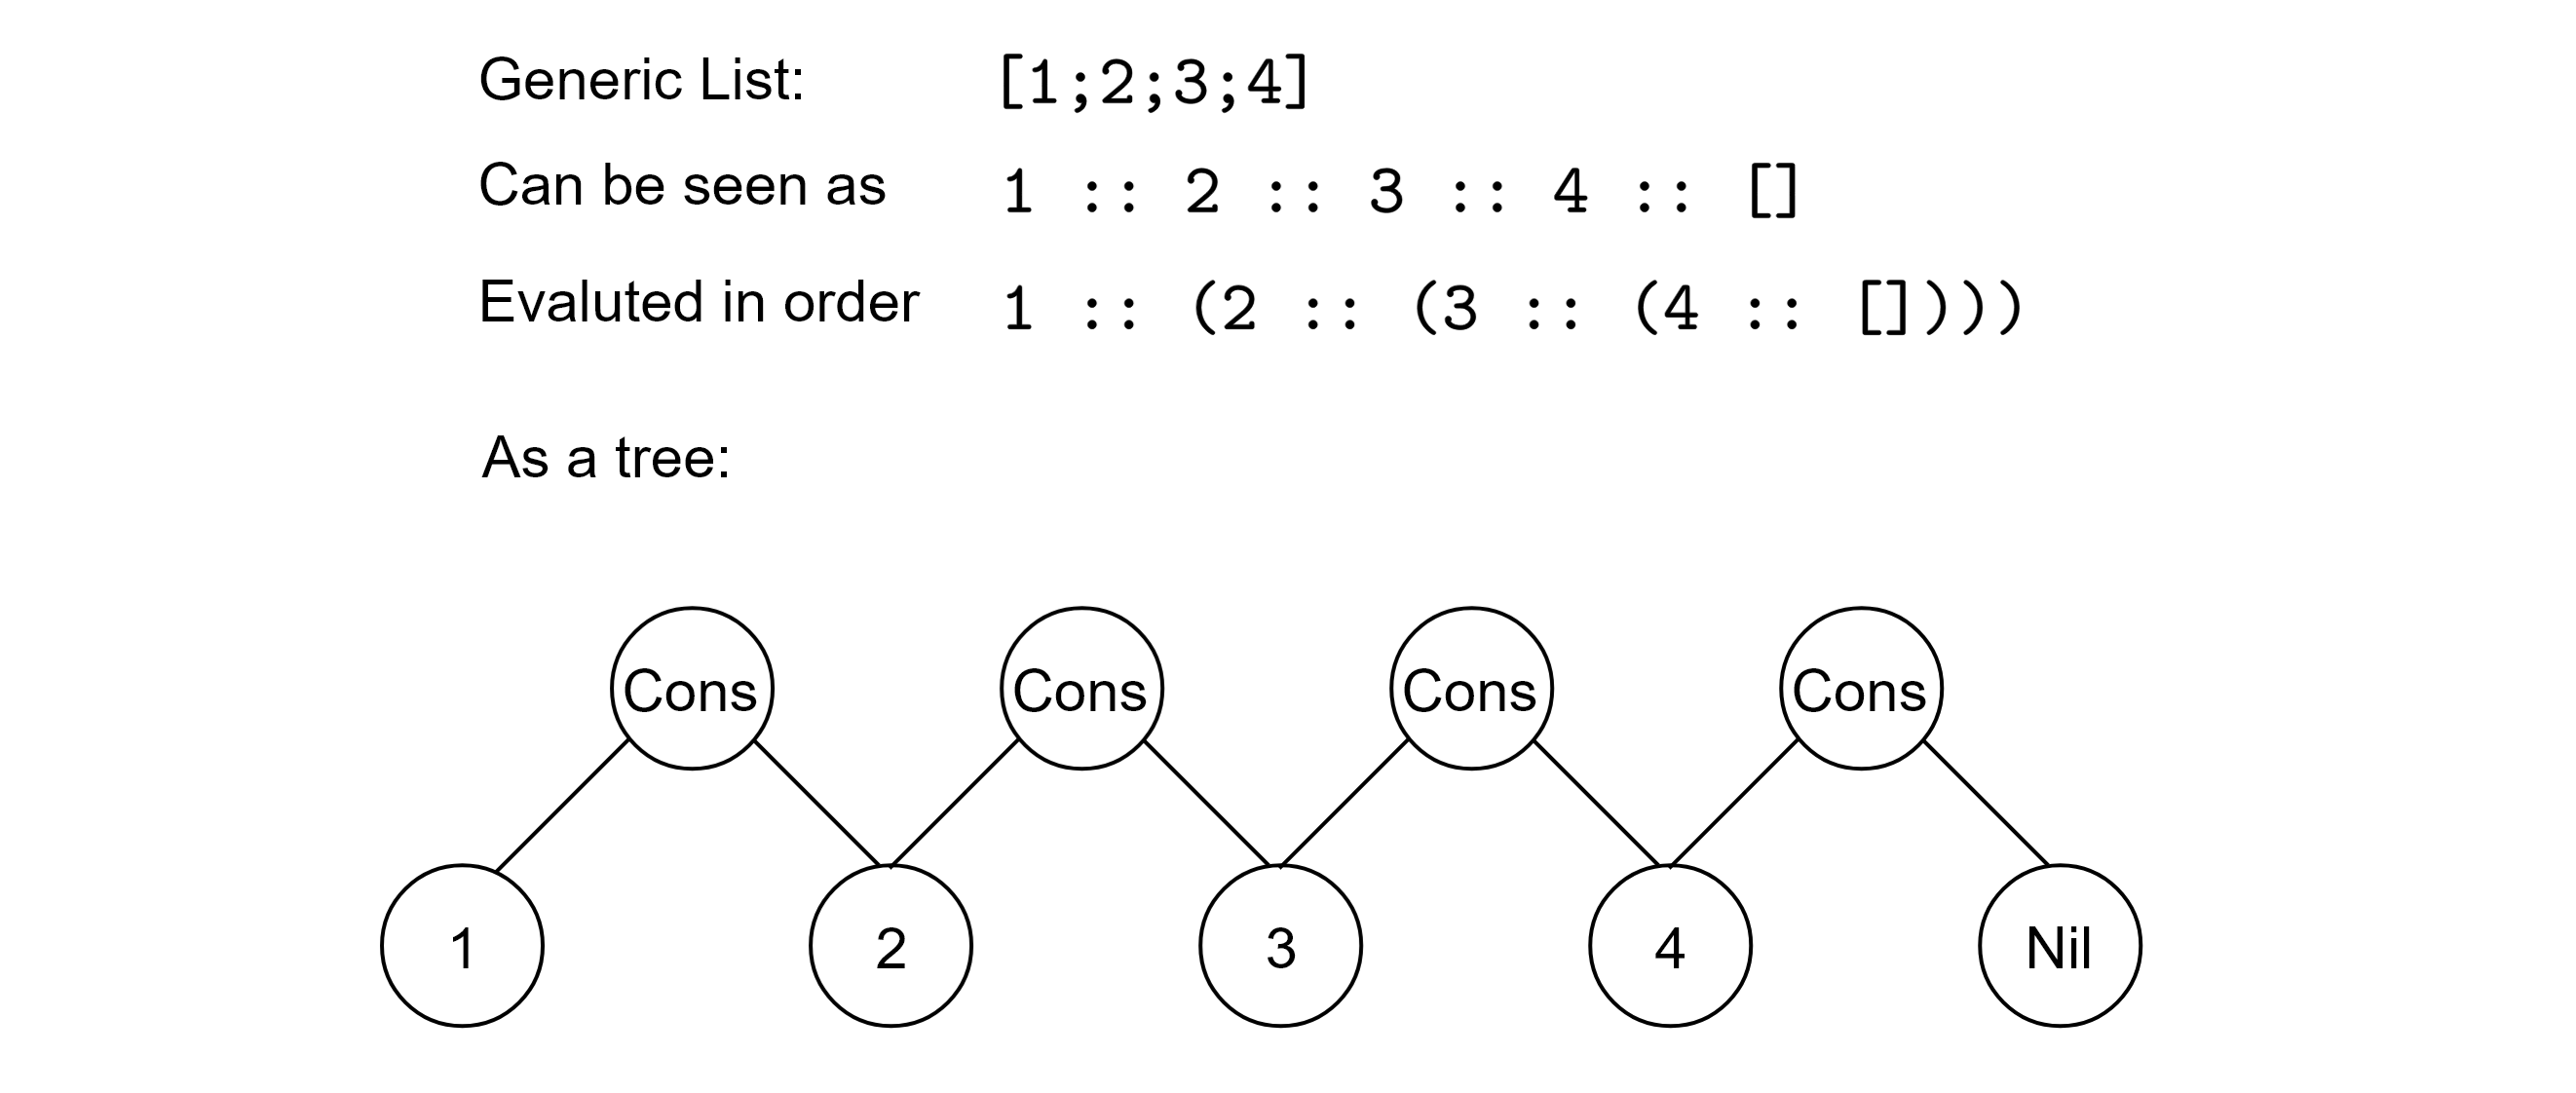
\includegraphics[width=1.1\textwidth]{Sections/adt/cons.png}
    \caption{Ocaml list representations.}
\end{figure}

\noindent
We can represent this of an integer list as either being,
\begin{itemize}
    \item \textbf{Base case}: Empty (\snippet{Nil})
    \item \textbf{Recursive case}: An Integer entry with reference to another entry (\snippet{int * intlist}), for which we label \snippet{Cons}.
\end{itemize}

\noindent
In essence, a list is actually a type of tree structure, where each node has a value and a reference to the next node. And that in reality, we may 
represent lists, trees, and graphs as an Algebraic Data Type.

\newpage 

\noindent
For instance, binary tree traversal can be represented as follows:

\begin{Example}
    We can define a binary tree as a recursive \texttt{ADT} in \texttt{OCaml}, where each node contains a value and references to left and right subtrees.

    \begin{lstlisting}[language=OCaml, caption={Binary Tree Definition and Traversals}, numbers=none]
    (* Define a binary tree type *)
    type 'a btree =
      | Empty
      | Node of 'a * 'a btree * 'a btree

    (* Example tree *)
    let example_tree =
      Node (1,
        Node (2, Node (4, Empty, Empty), Node (5, Empty, Empty)),
        Node (3, Node (6, Empty, Empty), Node (7, Empty, Empty))
      )

    (* Preorder traversal: Root -> Left -> Right *)
    let rec preorder t =
      match t with
      | Empty -> []
      | Node (v, left, right) -> [v] @ preorder left @ preorder right

    (* Inorder traversal: Left -> Root -> Right *)
    let rec inorder t =
      match t with
      | Empty -> []
      | Node (v, left, right) -> inorder left @ [v] @ inorder right

    (* Postorder traversal: Left -> Right -> Root *)
    let rec postorder t =
      match t with
      | Empty -> []
      | Node (v, left, right) -> postorder left @ postorder right @ [v]

    (* Example usage *)
    let _ =
      let pre = preorder example_tree in
      let inord = inorder example_tree in
      let post = postorder example_tree in
      (pre, inord, post) 
    (* Outputs: 
    ([1; 2; 4; 5; 3; 6; 7], [4; 2; 5; 1; 6; 3; 7], [4; 5; 2; 6; 7; 3; 1])
    *)
    \end{lstlisting}
\end{Example}

\newpage 

\noindent
We may use recursive ADTs to model expressions. Take for instance a basic arithmetic expression:
\begin{figure}[h]
    \centering
    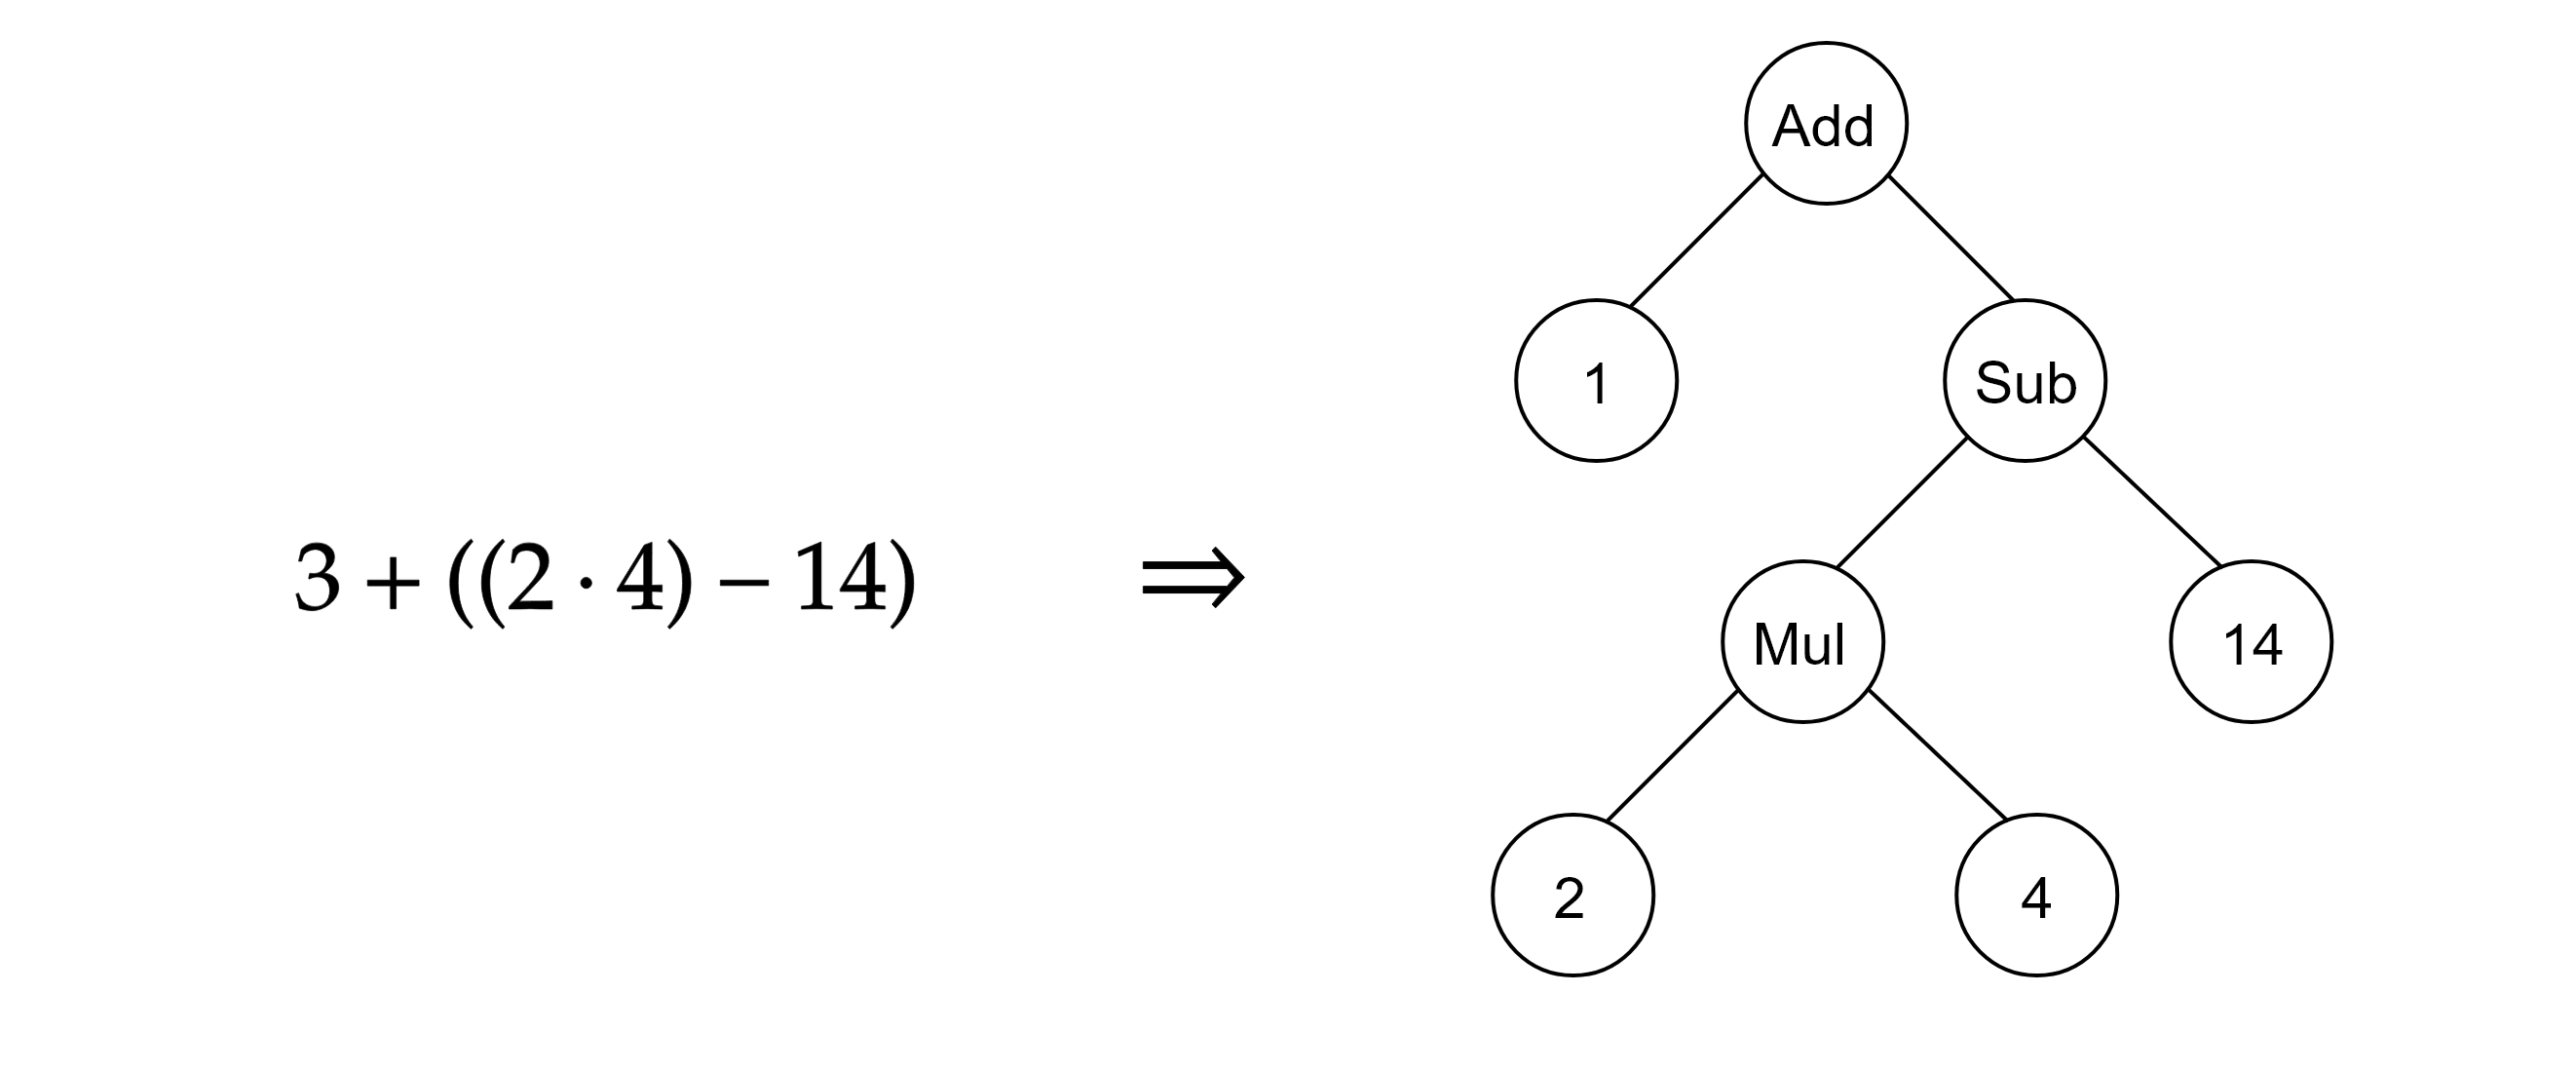
\includegraphics[width=1\textwidth]{Sections/adt/expr.png}
    \caption{Arithmetic expression tree.}
\end{figure}

\vspace{-1em}
\begin{Example}[Arithmetic Data Type]

    We define an arithmetic data type for Addition, Multiplication, and Subtraction of integers:
    \begin{lstlisting}[language=OCaml, caption={Arithmetic Expression Definition}, numbers=none]
    type expr =
      | Num of int
      | Add of expr * expr
      | Mul of expr * expr
      | Sub of expr * expr
    
    let _ = Add (Val 3, Sub (Mul (Val 2, Val 4), Val 14))
    (* Renders:      3 + ((2 * 4) - 14)                *)
    \end{lstlisting}
\end{Example}

\subsection{Parametric \& Polymorphic Types}
\noindent
Now what if we want to create a generic list that can store any type of value? In this case, we must parametrize the type definition.
\begin{Def}[Parametric Types]

    Parametric types are types that can take one or more type parameters. They are useful for creating generic data structures that can store values of any type.
\end{Def}

\newpage 

\begin{Example}[Parametric List]

    We can define a parametric list in \texttt{OCaml} that can store values of any type:
    \begin{lstlisting}[language=OCaml, caption={Parametric List Definition}, numbers=none]
    type 'a list =
      | Nil
      | Cons of 'a * 'a list

    let example_ints = Cons (1, Cons (2, Cons (3, Nil)))
    let example_strings = Cons ("a", Cons ("b", Cons ("c", Nil)))
    \end{lstlisting}

    \noindent
    Where \snippet{'a} is a type parameter and \snippet{list} is the type constructor.
\end{Example}

\noindent
Making the type generic also makes it polymorphic, meaning it can store values of any type. This is useful for creating reusable data structures.
\begin{Def}[Polymorphic Types]

    \textbf{Polymorphism} is the ability of a function or data type to operate on values of different types. \textbf{Parametric polymorphism} refers to functions or data types that are generic and can operate on values of any type.
\end{Def}

There is no overloading on types in \texttt{OCaml}:
\begin{Def}[Ad-Hoc Polymorphism]

    \textbf{Ad-hoc polymorphism} refers to a type of polymorphism where a function can be defined multiple times with different type signatures, allowing it to operate on different types using \textit{distinct implementations}.

    Some languages, such as C++ (via function overloading) and Haskell (via type classes), support ad-hoc polymorphism. However, \textbf{OCaml does not support ad-hoc polymorphism} because function overloading is not allowed—redefining a function replaces the previous definition.\\
    \begin{lstlisting}[language=OCaml, caption={No Overloading in OCaml}, numbers=none]
    (* The following isn't possible *)
    let add (a : int) (b : int) : int = a + b
    let add (a : string) (b : string) : string = a ^ b (* Overwrite *)
    let add (a : 'a list) (b : 'a list) : 'a list = a @ b (* Overwrites *)
    \end{lstlisting}
\end{Def}

\newpage 

\begin{Tip} Tony Hoare calls his invention of the
null pointer a ``billion-dollar mistake''
OCaml doesn't have null pointers\\
\noindent
\rule{\textwidth}{0.4pt}
\textit{I call it my billion-dollar mistake. It was the invention of the null
reference in 1965. At that time, I was designing the first comprehensive type
system for references in an object oriented language (ALGOL W). My goal was to
ensure that all use of references should be absolutely safe, with checking
performed automatically by the compiler. But I couldn't resist the temptation
to put in a null reference, simply because it was so easy to implement. This
has led to innumerable errors, vulnerabilities, and system crashes, which have
probably caused a billion dollars of pain and damage in the last forty years.}\\
-- Tony Hoare, inventor of null pointers
\end{Tip}



\chapter{Higher-Order Programming}
\section{Function Order}
In Higher-Order Programming, classes of values are established.

\begin{Def}[First-Class Values]

    \noindent
    A \textbf{first-class value} in a programming language is an entity that can be:
    \begin{itemize}
        \item \textbf{Assigned to variables}
        \item \textbf{Passed as an argument} to a function
        \item \textbf{Returned from a function}
        \item \textbf{Stored in data structures}
    \end{itemize}

    \noindent
    In \texttt{OCaml}, \textbf{functions are first-class values}, meaning they can be used like any other value. This allows for:
    \begin{itemize}
        \item Defining functions as values using \texttt{let}
        \item Passing functions as arguments to other functions
        \item Returning functions from other functions (closures)
    \end{itemize}

    \noindent
    However, \textbf{types are not first-class in OCaml}, meaning they cannot be manipulated as runtime values (e.g., dynamically created or passed as arguments).
\end{Def}

\noindent 
Passing functions to other functions is where the idea of \textbf{higher-order functions} comes into play.
\begin{Def}[Higher-Order Functions]

    \noindent
    A \textbf{higher-order function} is a function that:
    \begin{itemize}
        \item \textbf{Takes one or more functions as arguments}
        \item \textbf{Returns a function as a result}
    \end{itemize}

    \noindent
    We've discussed such functions before in Subsection (\ref{subsec:func-ocaml}). E.g.,
    (\texttt{fun f x -> f x}) is\\ (\texttt{fun f -> fun x -> f x}) where the first function returns and takes a function as an argument.
    Recall (\texttt{f x}) is a function application, where (\texttt{f}) is a function value.

\end{Def}

\newpage 


\begin{Def}[Order of Functions]
    
    The concept of ``higher-order'' extends beyond first-order functions, which take and return only values. A function's \textbf{order} is determined by how many levels of function application it involves:
    \begin{itemize}
        \item \textbf{1st order}: \texttt{int}
        \item \textbf{2nd order}: \texttt{int -> int}
        \item \textbf{3rd order}: \texttt{(int -> int) -> int}
        \item \textbf{4th order}: \texttt{((int -> int) -> int) -> int}
    \end{itemize}
    
    In theory, this hierarchy can extend infinitely, but in practice, functions rarely exceed \textbf{third or fourth order}.
\end{Def}

\begin{Tip}[What Does ''Higher-Order" Mean?]
    \textit{``Like things and functions are different, so are functions whose arguments are functions 
    \textbf{radically different} from functions whose arguments \textbf{must be things}. 
    I call the latter functions of first order, the former functions of second order.''}\\

    \noindent
    -- Gottlob Frege
\end{Tip}

\subsection{The Abstraction Principle: Maps, Filters, Folds}
The \textbf{Abstraction Principle} is a fundamental concept in computer science that states:
\begin{Def}[Abstraction Principle]

    The \textbf{Abstraction Principle} states that programs should be structured by separating \textbf{core functionality} from specific details.\\

    \noindent
    This principle is applied by:
    \begin{itemize}
        \item \textbf{Abstracting core functionality} to improve reusability and modularity.
        \item Using \textbf{higher-order functions} to \textbf{parametrize} behavior based on specific problem requirements.
        \item Understanding the \textbf{algebra of programming}, which helps reason about program structure and transformations.
    \end{itemize}

    \noindent
    Following this principle results in more \textbf{flexible, maintainable, and reusable} programs.
\end{Def}

\noindent
We'll discuss three common patterns we see a lot in programmings \textbf{Maps}, \textbf{Filters}, and \textbf{Folds}.

\newpage 

\noindent

\begin{Def}[Map Function]

    Given a function \( f \) and a list \([x_1, x_2, \dots, x_n]\), the \textbf{map} function produces:
    \[
    \texttt{map } f [x_1, x_2, \dots, x_n] = [f(x_1), f(x_2), \dots, f(x_n)]
    \]
    \noindent
    I.e., it applies \( f \) to each element of the list, returning a new list with the results.\\
    \begin{lstlisting}[language=OCaml, caption={Ocaml Implementation of Map}, numbers=none]
    let rec map f lst =
      match lst with
      | [] -> []
      | x :: xs -> f x :: map f xs

    (* Example usage *)
    let doubled = map (fun x -> x * 2) [1; 2; 3]  (* Returns [2; 4; 6] *)
    \end{lstlisting}

    \noindent
    The \textbf{map} function abstracts over how we apply a function to each element of a list, allowing us to reuse the same logic for different functions.
\end{Def}

\noindent
\begin{Def}[Filter Function]

    Given a predicate function \( p \) and a list \([x_1, x_2, \dots, x_n]\), the \textbf{filter} function produces:
    \[
    \texttt{filter } p\ [x_1, x_2, \dots, x_n] = [x_i \mid p(x_i) \texttt{ is true}]
    \]
    \noindent
    I.e., it returns a new list containing only elements for which \( p \) evaluates to \texttt{true}.\\

    \begin{lstlisting}[language=OCaml, caption={Ocaml Implementation of Filter}, numbers=none]
    let rec filter p lst =
      match lst with
      | [] -> []
      | x :: xs ->  (if p x then [x] else []) @ filter p xs

    (* Example usage *)
    let evens = filter (fun x -> x mod 2 = 0) [1; 2; 3; 4; 5]
    (* Returns [2; 4] *)
    \end{lstlisting}

    \noindent
    The \textbf{filter} function abstracts over how we select elements from a list, allowing us to express selection logic concisely.
\end{Def}

\newpage 

\noindent
\begin{Def}[Fold Functions]

    Given a binary function \( f \), an initial accumulator value \( a_0 \), and a list \([x_1, x_2, \dots, x_n]\), the \textbf{fold} functions \texttt{fold\_left} and \texttt{fold\_right} reduce the list to a single value by combining elements recursively.\\

    \noindent
    The \textbf{fold left} function applies \( f \) from left to right (recursive statement on the right):
    \[
    \texttt{fold\_left } (-) \ a_0\ [x_1, x_2, \dots, x_n] = (((a_0 - x_1) - x_2) \dots - x_n)
    \]

    \noindent
    I.e., we dig to the base case hitting $x_n$, then start unraveling, tunneling \textbf{left} back to ($x_1$, $a_0$).
    \begin{lstlisting}[language=OCaml, caption={Ocaml Implementation of Fold\_Left}, numbers=none]
    let rec fold_left f acc lst =
      match lst with
      | [] -> acc
      | x :: xs -> fold_left f (f acc x) xs

    (* Example usage *)
    let subtract = fold_left (-) 10 [1; 2; 3]  
    (* Returns 4, since ((10 - 1) - 2) - 3 = 4 *)
    \end{lstlisting}

    \vspace{1em}
    \noindent
    The \textbf{fold right} function applies \( f \) from right to left (recursive statement on the left):
    \[
    \texttt{fold\_right } (-) \ a_0\ [x_1, x_2, \dots, x_n] = (x_1 - (x_2 - (\dots - (x_n - a_0))))
    \]

    \noindent
    I.e., we dig to the base case hitting ($x_n, a_0$), we start boxing up values pushing them to the \textbf{right}, building up to the top layer, $x_1$.
    \begin{lstlisting}[language=OCaml, caption={Ocaml Implementation of Fold\_Right}, numbers=none]
    let rec fold_right f lst acc =
      match lst with
      | [] -> acc
      | x :: xs -> f x (fold_right f xs acc)

    (* Example usage *)
    let subtract = fold_right (-) [1; 2; 3] 10  
    (* Returns -8, since 1 - (2 - (3 - 10)) = -8 *)
    \end{lstlisting}
\end{Def}

\begin{Tip}
    Think in opposition: fold left (recursive statement on the right), fold right (recursive statement on the left).
\end{Tip}

\newpage 

\noindent
To illustrate the difference between \texttt{fold\_left} and \texttt{fold\_right}, consider the following illustration:

\begin{figure}[h]
    \centering
    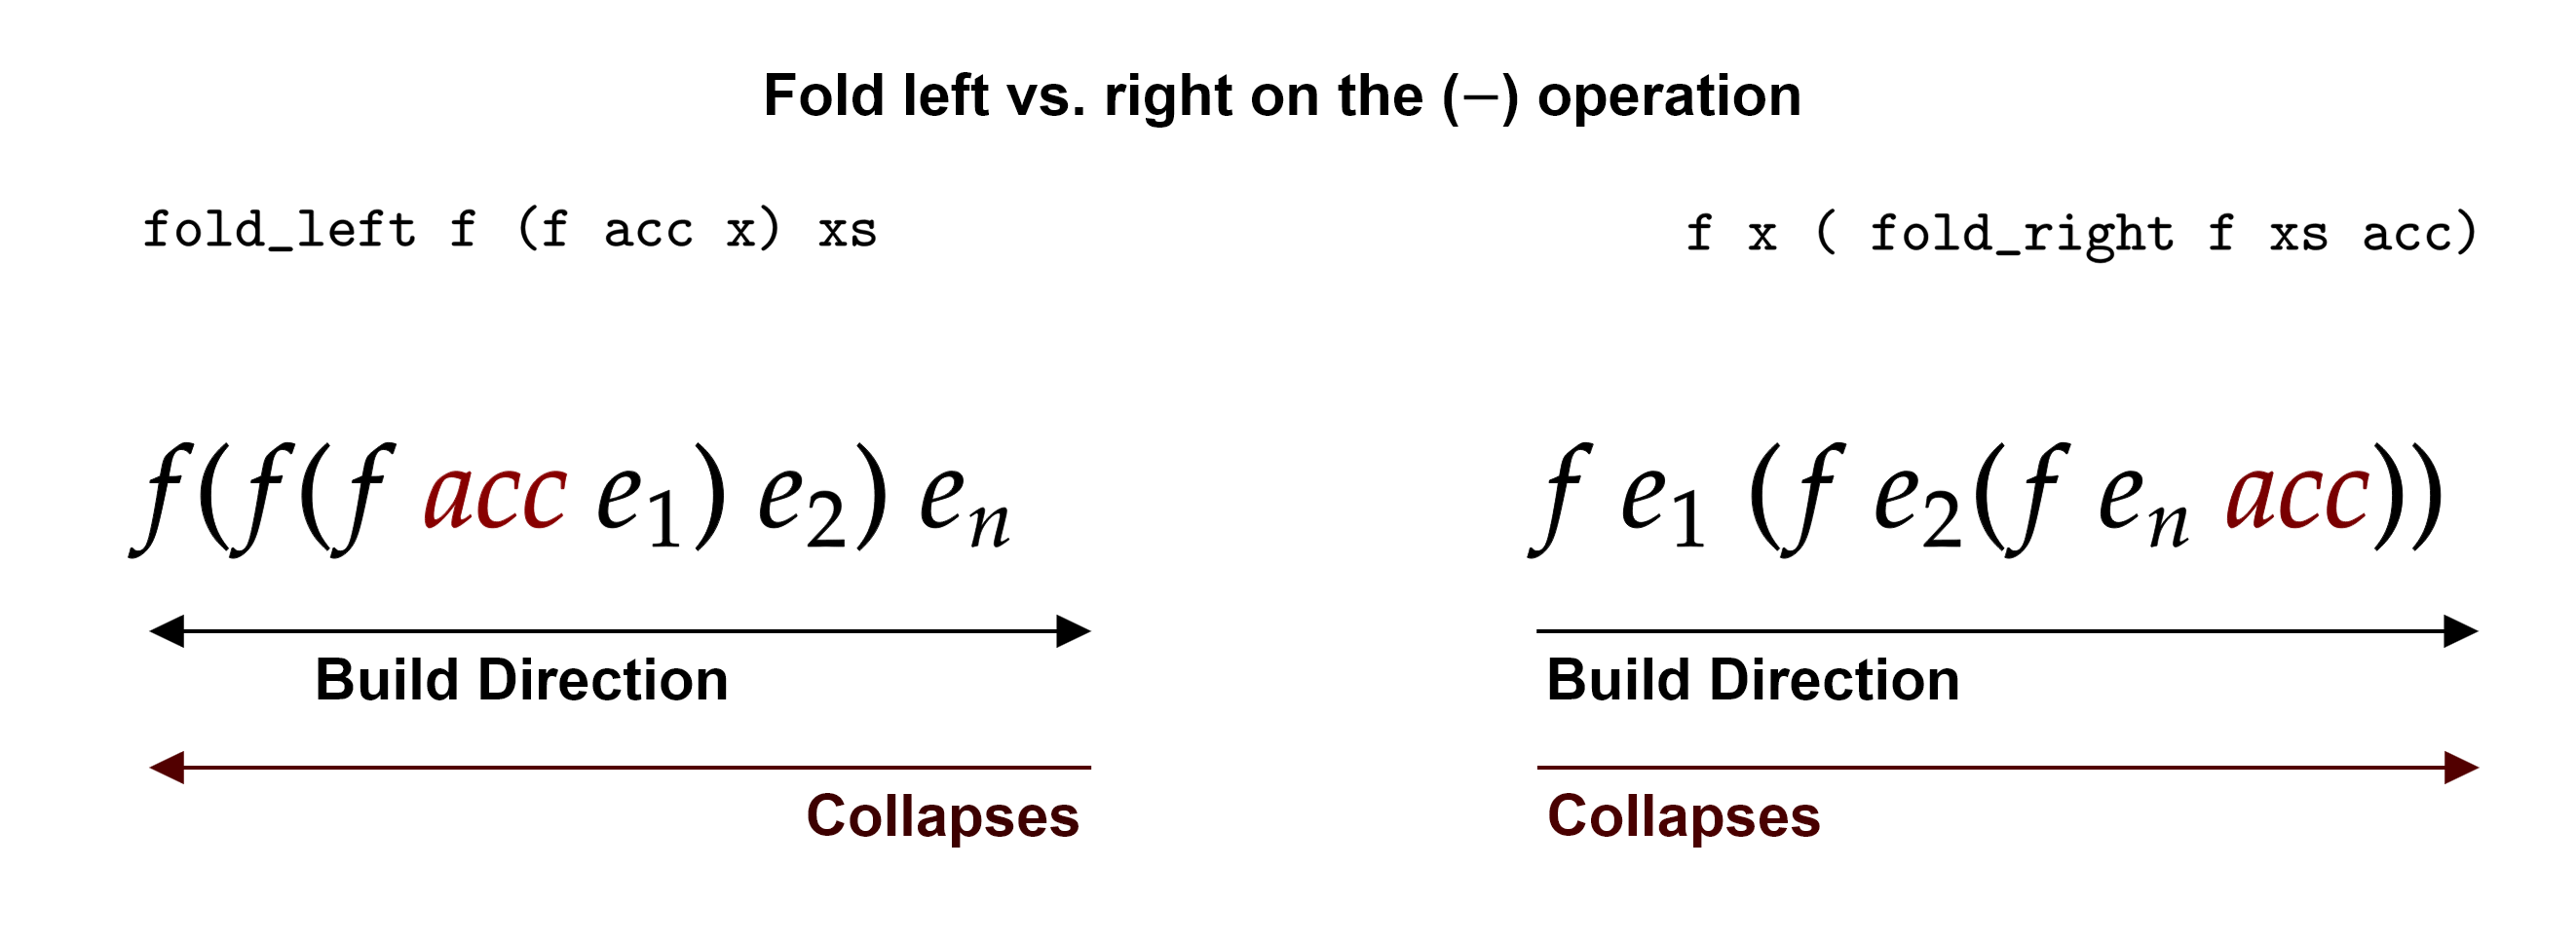
\includegraphics[width=0.8\textwidth]{Sections/order/fold.png}
    \caption{Fold Left vs. Fold Right}
\end{figure}

\noindent
In both, we still build from the base case/last element to the front of the list. So above, we are always building from right to left.
The difference: 

\begin{itemize}
    \item \textbf{Fold Left}: We tunnel in from right to left, applying the accumulator to the first element.
    \item \textbf{Fold Right}: We box up values from left to right, applying the accumulator to the last element.
\end{itemize}

\noindent
Though again for emphasis, the original naming intention was: 
\begin{itemize}
    \item \textbf{Fold Left}: Apply the accumulator from the \textbf{left} of the list to the right.
    \item \textbf{Fold Right}: Apply the accumulator from the \textbf{right} of the list to the left.
\end{itemize}




\newpage
\section{Handling Errors \& Testing: Results, Bind, \& Monads}

\subsection{Monads \& Binds}
\begin{Def}[Monads]

    A \textbf{monad} extends the functionality of a type by wrapping it in a monadic context.
    For example, we could extend the type \snippet{int} to include a \snippet{Null} type by wrapping it in a
    a custom type, \snippet{type myNumber = Null | Int of int}.
    Monads consists of:
    \begin{itemize}
        \item A \textbf{type constructor} \( M \) that wraps values.
        \item A \textbf{unit} (or \texttt{return}) function that lifts a value into the monadic context:
        \[
        \eta : A \to M(A).
        \]
        \noindent
        Where \(\eta\) is our unit function taking $A$ and wrapping it in the monadic context $M(A)$.
        \item A \textbf{bind} function that ensures the monadic structure is maintained between operations:
        \[
        \mu : M(A) \times (A \to M(B)) \to M(B),
        \]
        \noindent
        Where \(\mu\) is our bind function. Recall,
        the ($\times$) is the cartesian product of the two types, i.e., a tuple of the two objects.
    \end{itemize}
\noindent
    A monad satisfies the \textbf{monad laws}:
    \begin{enumerate}
        \item \textbf{Left Identity:} \( \left(\eta(x) \texttt{ bind } f\right) = f(x) \). Binding a monadic value to a function is equivalent to applying the function to the value.
        \item \textbf{Right Identity:} \( (m \texttt{ bind } \eta) = m \). Binding a monadic value to the unit function is equivalent to the original value.
        \item \textbf{Associativity:} \( (m \texttt{ bind } f) \texttt{ bind } g = m \texttt{ bind } ( \lambda x. f(x) \texttt{ bind } g) \). The order of binding functions does not matter.
    \end{enumerate}

    \noindent
    \rule{\textwidth}{0.4pt}\\

    \noindent
    In an OCaml context, \snippet{options} are an example of a monad.
    \begin{lstlisting}[language=OCaml, caption={Option Monad in OCaml}, numbers=none]
    type 'a option = 
    | Some of 'a 
    | None    
    \end{lstlisting}
    \noindent
    For the Option monad, \snippet{Some} serves as the unit function, as it takes a value of type \snippet{'a} and lifts it into the monadic context \snippet{'a option}.
    Both \snippet{Some} and \snippet{None} are constructors for the \snippet{option} type.
    \end{Def}
    
    \newpage 
    \vspace{2em}

    \begin{Def}[Bind with \texttt{let*} in OCaml]

\label{def:let*}

        The \snippet{let*} operator corresponds to the monad's bind function. The bind operation could be thought of as ``try to unwrap $x$ and then do $f$''.
        For example, in the \snippet{option} monad:
        
        \begin{lstlisting}[language=OCaml, numbers=none]
        (* Define the bind function for option *)
        let bind opt f =
          match opt with
          | Some x -> f x
          | None -> None
        (* Define the let* operator *)
        let ( let* ) = bind
        \end{lstlisting}
    
    
        \noindent
        Though OCaml has saved us the trouble of defining the bind function, via the \snippet{.bind} function in ocaml.
        \begin{lstlisting}[language=OCaml, numbers=none]
        let ( let* ) = Option.bind
        \end{lstlisting}
    
        \noindent
        \textbf{Using \snippet{let*} in Monadic Expressions:}  
        Once \snippet{let*} is defined, it allows chaining monadic computations naturally. Consider an example using the \snippet{option} monad:
    
        \begin{lstlisting}[language=OCaml, numbers=none]
    (* Using let* to chain option operations *)
    let foo =
        let ( let* ) = Option.bind in
        let* x = Some 4 in
        let* y = Some 3 in
        let* z = Some 2 in
        Some (x + y + z);
    
    (* foo evaluates to Some 9 *)
        \end{lstlisting}

        \noindent
        This could be seen as the below nested match expressions:
        \begin{lstlisting}[language=OCaml, numbers=none]
            match Some 4 with
            | None -> None
            | Some x -> (
                match Some 3 with
                | None -> None
                | Some y -> (
                    match Some 2 with
                    | None -> None
                    | Some z -> Some (x + y + z)
                    )
                )
        \end{lstlisting}
        \noindent
        This is for curiosity sake, and conceptually would be simpler to think of bind as a means of unwrapping the monad
        to preform some operation before rewrapping it.
    
    \end{Def}
    
    \newpage 

    \begin{Def}[Result Type in OCaml]
        
        The \snippet{result} type is another example of a monad in OCaml that represents computations which may \underline{\textbf{succeed} or \textbf{fail}}. Unlike the \snippet{option} type which only indicates presence or absence, \snippet{result} provides information about why a computation failed.
        
        \begin{lstlisting}[language=OCaml, caption={Result Type in OCaml}, numbers=none]
        type ('a, 'e) result = 
        | Ok of 'a      (* Success case with value of type 'a *)
        | Error of 'e   (* Error case with error of type 'e *)
        \end{lstlisting}
        
        \noindent
        For the Result monad:
        \begin{itemize}
            \item \snippet{Ok} serves as the unit function, lifting a value into the success context
            \item The bind operation sequences computations while handling errors
        \end{itemize}
        
        \noindent
        \textbf{Using Result with Bind:}
        
        \begin{lstlisting}[language=OCaml, numbers=none]
        (* Define the bind operator for result *)
        let ( let* ) = Result.bind
        
        (* Example chaining result operations *)
        let divide x y =
          if y = 0 then Error "Division by zero"
          else Ok (x / y)
        
        let computation x y z =
          let* result1 = divide x y in
          let* result2 = divide result1 z in
          Ok (result2 * 2)
        
        (* Success case: computation 10 2 1 = Ok 10 *)
        (* Error case:   computation 10 0 1 = Error "Division by zero" *)
        \end{lstlisting}
        
        \noindent
        In the example above, if any Error occurs it short-circuits the computation and returns the error immediately.
        Recall the nested match in the \snippet{let*} Definition (\ref{def:let*}), this is conceptually similar to that.

    \end{Def}

    \newpage 

    \subsection{Testing \& Ounit2}
    This section is about testing as a means of ensuring the correctness of our code down the development pipeline.

    \begin{Def}[Types of Testing]

        In software development, testing can be categorized into several hierarchical levels, with the three primary types being:
        
        \begin{enumerate}
            \item \textbf{Unit Testing:} Tests individual components (functions, modules) in isolation.
                        \begin{itemize}
                            \item Focuses on verifying that each unit of code works as expected
                            \item Typically automated and run frequently during development
                        \end{itemize}
                        
                        \item \textbf{Integration Testing:} Tests interactions between components.
                        \begin{itemize}
                            \item Verifies that different units work together correctly
                            \item Components may be nested or distributed across the simulated workflow
                        \end{itemize}
                        
                        \item \textbf{End-to-End (E2E) Testing:} Tests the application from start to finish.
                        \begin{itemize}
                            \item Simulates real user scenarios and workflows
                            \item Verifies the system works in real-world conditions with actual data
                            \item Tests the entire application stack including UI, API, database connections, etc.
                        \end{itemize}
        \end{enumerate}
        \noindent
        In software development \textbf{testing frameworks} are used to help speed up the process of writing and running tests.
        These are libraries that provide tools for writing, organizing, and running tests.
    \end{Def}
    
    \begin{Tip} While academic settings often focus on the theoretical aspects of testing, industry practices are typically more nuanced and pragmatic. In many professional software development environments:

        \begin{itemize}
            \item \textbf{Test-Driven Development (TDD)} has gained significant traction, where developers write tests before implementing functionality. This approach often leads to more testable and modular code, but requires discipline to maintain.
            
            \item \textbf{Continuous Integration (CI)} systems run tests automatically when code changes are committed, catching regressions early in the development cycle. Companies may run thousands of tests multiple times daily.
            
            \item The \textbf{testing pyramid} concept is widely followed, with many unit tests forming the base, fewer integration tests in the middle, and even fewer E2E tests at the top—balancing thoroughness with execution speed.
    \end{itemize}
    \end{Tip}
 
    \newpage

    \noindent
    We choose \textbf{OUnit2} for testing, which should have been installed in Sub-section (\ref{subsec:opam_packages}).
    Though not the most featured testing framework, it is simple and easy to use.

    \vspace{-0em}
    \begin{Def}[OUnit2 in OCaml]

        \textbf{OUnit2} is a unit testing framework for OCaml that allows developers to write and run tests to verify code correctness.
        To use OUnit2, add it as a dependency in your dune project file:
        \begin{lstlisting}[language=OCaml, numbers=none]
        (test
         (name test_program)
         (libraries ounit2))
        \end{lstlisting}

        \noindent
        \textbf{Key OUnit2 Functions:}
        \begin{itemize}
            \item \snippet{(>::)} - Creates a labelled test
            \item \snippet{(>:::)} - Creates a labelled test suite
            \item \snippet{assert\_equal} - Compares two values in a unit test
            \item \snippet{assert\_raises} - Checks that an expression raises the expected exception
            \item \snippet{run\_test\_tt\_main} - Runs a test suite
        \end{itemize}

        \noindent
        \textbf{Example OUnit2 Test:}
        \begin{lstlisting}[language=OCaml, numbers=none]
    open OUnit2

    (* Function to test *)
    let add x y = x + y

    (* Test cases *)
    let tests = 
        "test suite for addition" >:::
        [
        "adding two positive numbers" >:: (fun _ -> 
            assert_equal 5 (add 2 3));
        
        "adding zero" >:: (fun _ -> 
            assert_equal 7 (add 7 0));
            
        "testing exception" >:: (fun _ ->
            assert_raises (Failure "division by zero") 
            (fun () -> 1 / 0))
        ]

    (* Run the tests *)
    let () = run_test_tt_main tests
        \end{lstlisting}
    \end{Def}
\section{Modules In Ocaml}

This section details how OCaml deals with modular programming, including abstractions and interfaces.

\begin{Def}[Modular Programming]

Modular programming is a software design approach that emphasizes separating a program's functionality into independent, interchangeable modules,
which are composed of three key elements:

\begin{enumerate}
    \item \textbf{Namespaces:} A way of separating code into logical units of functions, types, and values together while avoiding name conflicts.
    
    \item \textbf{Abstraction/Encapsulation:} A way of abstracting away implementation details and organizing core functionality. This creates a clear boundary between the module's intent and its implementation for clarity.
    
    \item \textbf{Code Reuse:} Well-designed modules can serve as reusable components across multiple projects, reducing duplication.
\end{enumerate}

\end{Def}

\begin{Def}[The (\texttt{module}) \& (\texttt{struct}) Keyword in OCaml]

    The \textbf{module} keyword in OCaml is used to define a collection of related code elements (types, values, functions) that are grouped together into a single namespace.

    \begin{lstlisting}[language=OCaml, numbers=none, caption= \textbf{Basic Module Syntax:}]
    module ModuleName = struct
    (* Types, values, and functions *)
    type t = int * int
    let create x y = (x, y)
    let add (x1, y1) (x2, y2) = (x1 + x2, y1 + y2)
    end
    \end{lstlisting}

    \noindent
    Where the \snippet{struct} keyword defines the collection of
    definitions under the module.
    Once defined, module elements are accessed using the dot notation:
    \begin{lstlisting}[language=OCaml, numbers=none]
    let point = ModuleName.create 10 20
    let sum = ModuleName.add point point
    \end{lstlisting}

    \noindent
    Multiple modules may be defined in a single file, and be used in and between other files.

\end{Def}

\newpage 

\begin{Def}[Module Access: (\texttt{open}) and Local Opens]
    OCaml provides multiple ways to access module contents:\\

    \noindent
    \textbf{Qualified access:} uses dot notation: \snippet{ModuleName.function\_name}\\
        
    \noindent
    \textbf{Global open:} brings all module contents into the current scope:
        \begin{lstlisting}[language=OCaml, numbers=none]
    (* All List functions now available without qualification *)
    open List  
    let x = map (fun x -> x * 2) [1; 2; 3]  (* No need for List.map *)
        \end{lstlisting}
        
    \noindent
    \textbf{Local open:} provides temporary access within a limited scope:
        \begin{lstlisting}[language=OCaml, numbers=none]
    (* Using Module.(expr) syntax *)
    let result = List.(
    map (fun x -> x * 2) [1; 2; 3]  
    (* List is open only in this scope *)
    )

    (* Outside the parentheses, module is not opened *)
    let standard = List.length [1; 2; 3]  (* Need qualification again *)
        \end{lstlisting}
 
\end{Def}

\begin{Def}[Module Signatures: (\texttt{sig}) \& (\texttt{module type})]
    
    Signatures are interfaces to modules. They 
    are created in \snippet{.mli} files:

    \begin{lstlisting}[language=OCaml, numbers=none]
    module type POINT = sig
      (* Abstract type - implementation hidden *)  
      type t              
      val private create : int -> int -> t
      val add : t -> t -> t
    end
    \end{lstlisting}

    \noindent
    The \snippet{val} keyword explains rather than defines like \snippet{let}. Signatures are then applied to modules to ensure they conform to the interface:
    
    \begin{lstlisting}[language=OCaml, numbers=none]
    module Point : POINT = struct
      type t = int * int
      let create x y = (x, y)
      let add (x1, y1) (x2, y2) = (x1 + x2, y1 + y2)
      
      (* This function is private as its not in the signature *)
      let sub x y = x - y 
    end
    \end{lstlisting}
\end{Def}

\begin{Def}[Module Helper Pattern for Data Structures]
    
    A common pattern in OCaml is to create helper functions inside modules to simplify working with complex data structures. 
    This approach makes code more concise and readable by providing shorthand notations for constructors.\\

    \noindent
    For example, with a binary tree:
    
    \begin{lstlisting}[language=OCaml, numbers=none]
    type 'a tree =
      | Leaf
      | Node of 'a * 'a tree * 'a tree

    module TreeExample = struct
      let l = Leaf
      let n l r = Node ((), l, r)
    end
    
    (* Using local open for concise tree construction *)
    let example = TreeExample.(n (n (n l l) l) (n l l))
    \end{lstlisting}
    
    \noindent
    Instead of writing the full constructor names repeatedly, the module provides shorthand aliases (\snippet{l} for \snippet{Leaf} and \snippet{n} for creating \snippet{Node}s). Combined with local opens, this makes tree construction much more readable than the equivalent:
    \begin{lstlisting}[language=OCaml, numbers=none]
    let example = Node ((), Node ((), Node ((), Leaf, Leaf), Leaf), Node ((), Leaf, Leaf))
    \end{lstlisting}
\end{Def}

\chapter{The Interpretation Pipeline}
\section{Formal Grammars}
\subsection{Defining a Language}
Now we introduce formal grammars as a way of building up our language.
This is similar to English, where we have a grammar system that tells us how to build sentences.
For example, we know the basic structure of a sentence is \textit{subject-verb-object}. \\

\noindent
We can write \textbf{linear} statements such as ``John hit the ball'', which has an underlying \textbf{hierarchical} structure that permits it:

\begin{figure}[h]
\centering
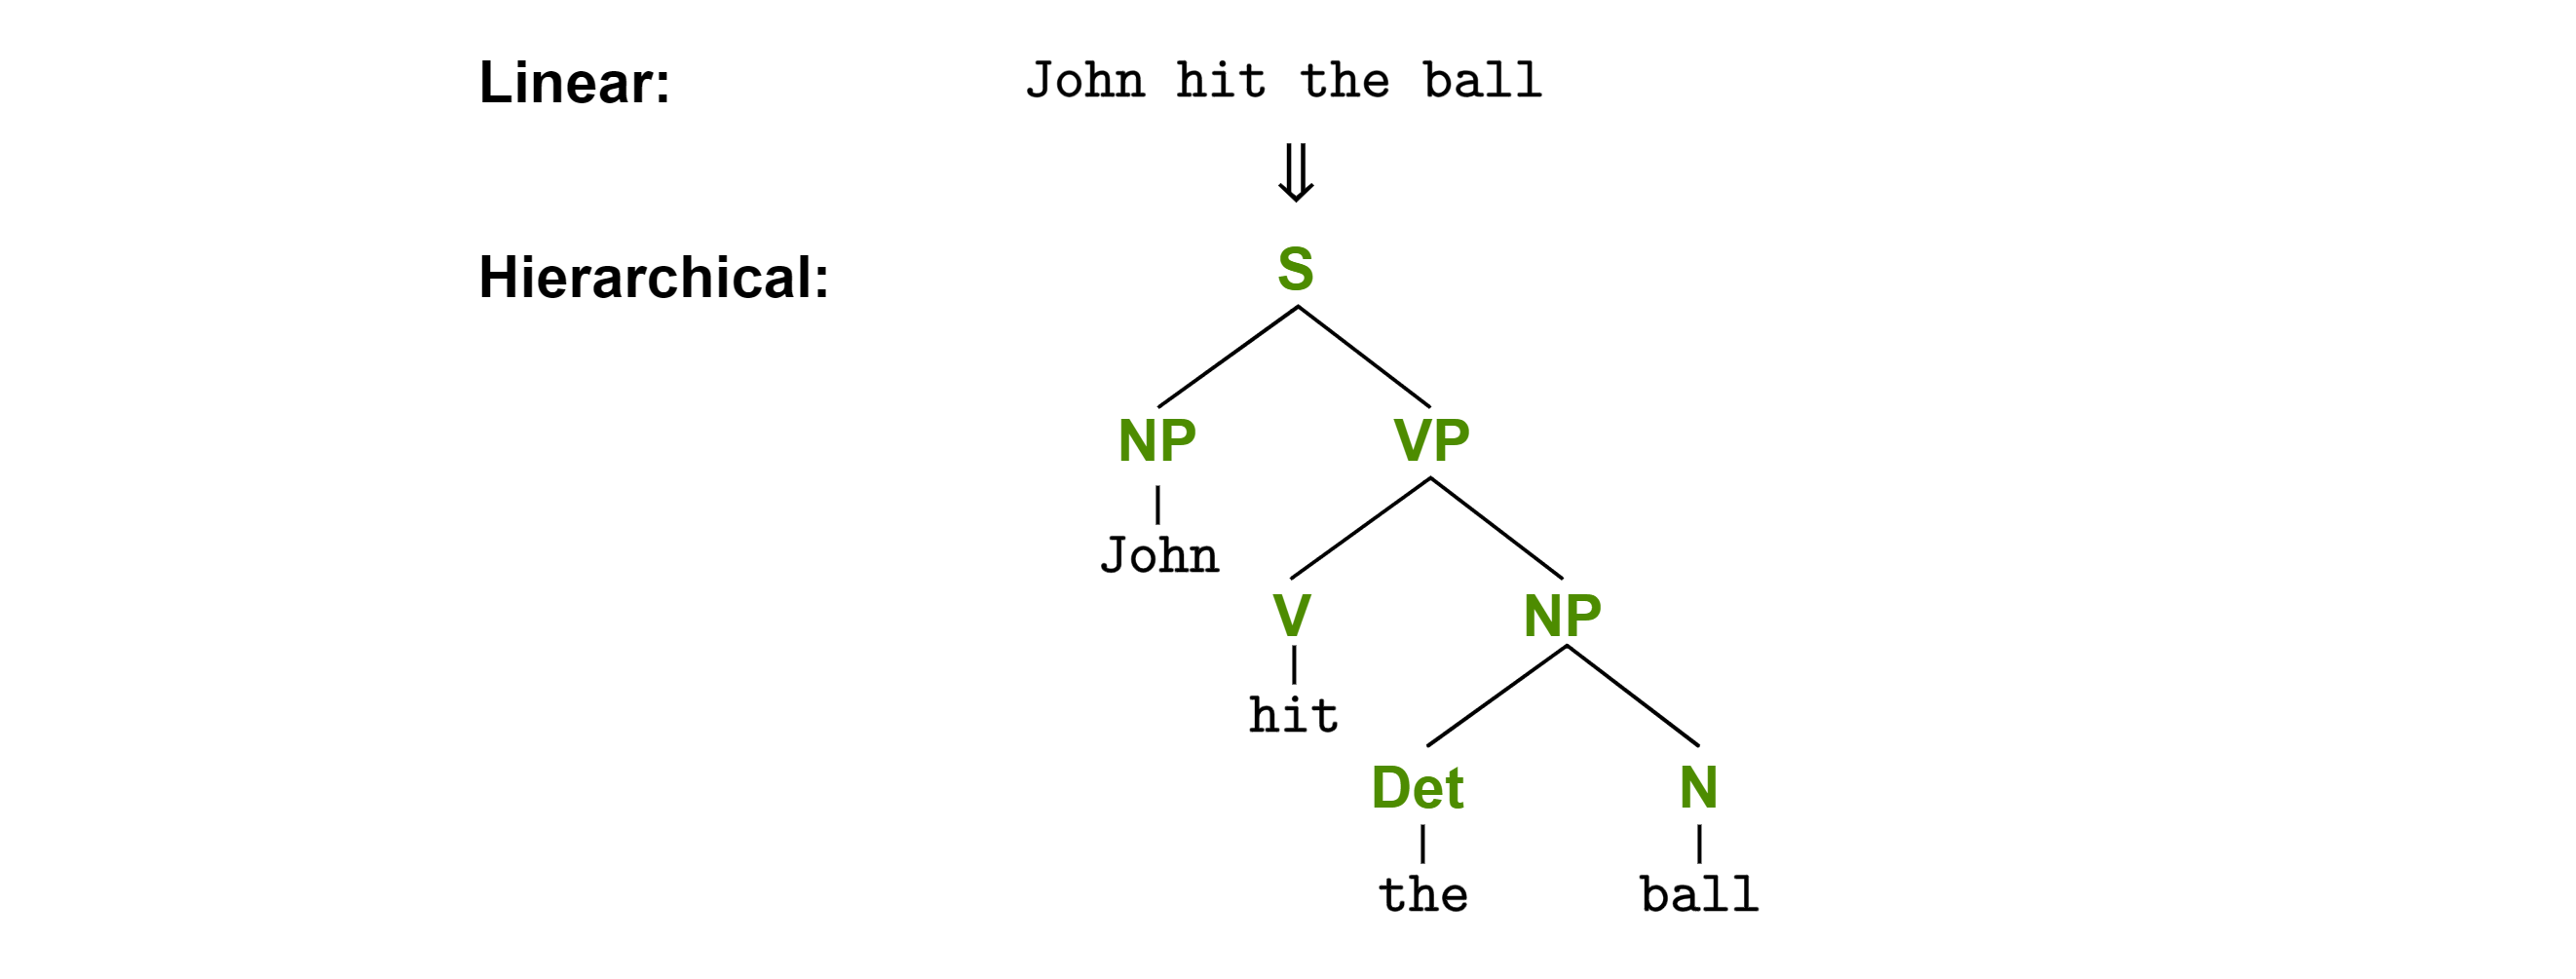
\includegraphics[width=1\textwidth]{Sections/Formal/eng.png}
\caption{The sentence ``John hit the ball'' has an underlying hierarchical structure of a tree. Here, \textbf{S}: Sentence (the root of the tree), \textbf{NP}: Noun Phrase (a phrase centered around a noun), \textbf{VP}: Verb Phrase (a phrase centered around a verb), \textbf{V}: Verb (the action in the sentence), \textbf{Det}: Determiner (words like ``the", ``a", ``an", which specify nouns), and \textbf{N}: Noun (person, place, thing, or idea).}
\end{figure}

\noindent
\textbf{Grammar vs. Semantics:} Notice the english sentence 

\begin{center}
\Large \textit{``Your air tied a toothbrush at school!''}
\end{center}

\noindent
is grammatically correct, but carries little to no meaning. In contrast, 
the sentence:

\begin{center}
\Large \textit{``Colorless the of allegator run am sleepily''}
\end{center}

\noindent
is perhaps an unsettling read, as it is not grammatically correct. \\

\newpage 

\noindent
The same way we can represent english sentences in a tree structure, is the same way we can represent programs. First 
we define the difference between an \textbf{interpreter} and a \textbf{compiler}.

\begin{Def}[Interpreter]

    An \textbf{interpreter} is a program that directly executes instructions written in a programming language without 
    requiring a machine code translation. The typical stages are:
    
    \begin{enumerate}
        \item \textbf{Lexical Analysis}: Reads a string of characters (program), converting it into tokens.
        \item \textbf{Syntax Analysis}: Parses these tokens to build an abstract syntax tree (AST).
        \item \textbf{Semantic Analysis}: Checks for semantic errors and annotates the AST.
        \item \textbf{Intermediate Representation (IR) Generation}: Converts the AST into an intermediate representation (IR) to facilitate execution.
        \item \textbf{Direct Execution}: Executes the IR or AST directly using an interpreter.
    \end{enumerate}
    
    \noindent
    Interpreted languages are \textbf{evaluated at runtime} (e.g., Python, Ruby, JavaScript). Some interpreters use an \textbf{AST-based execution}, while others generate an \textbf{IR} (e.g., Python's bytecode for the CPython interpreter).
    
    \end{Def}
    
    \begin{Def}[Compiler]
    
    A \textbf{compiler} is a program that translates code written in a high-level programming language into a lower-level language, typically machine code, to create an executable program. This involves several stages:
    
    \begin{enumerate}
        \item \textbf{Lexical Analysis}: Reads the source code and converts it into tokens.
        \item \textbf{Syntax Analysis}: Parses these tokens to construct an abstract syntax tree (AST).
        \item \textbf{Semantic Analysis}: Validates the AST against language rules and performs type checking.
        \item \textbf{Intermediate Representation (IR) Generation}: Transforms the AST into a lower-level representation that is easier to optimize and translate.
        \item \textbf{Optimization}: Enhances the IR to improve performance and efficiency.
        \item \textbf{Code Generation}: Translates the optimized IR into machine code or another target language.
    \end{enumerate}
    
    \noindent
    Compiled languages are \textbf{translated before runtime} (e.g., C, C++, Rust, OCaml). The \textbf{IR} plays a crucial role in optimizing the compilation process, as seen in LLVM or Java’s bytecode execution in the JVM.
    
    \end{Def}
   
\newpage 

\noindent
The following diagram illustrate the translation process of a compiler and an interpreter:

\vspace{2em}

\begin{figure}[h]
    \hspace{-2em}
    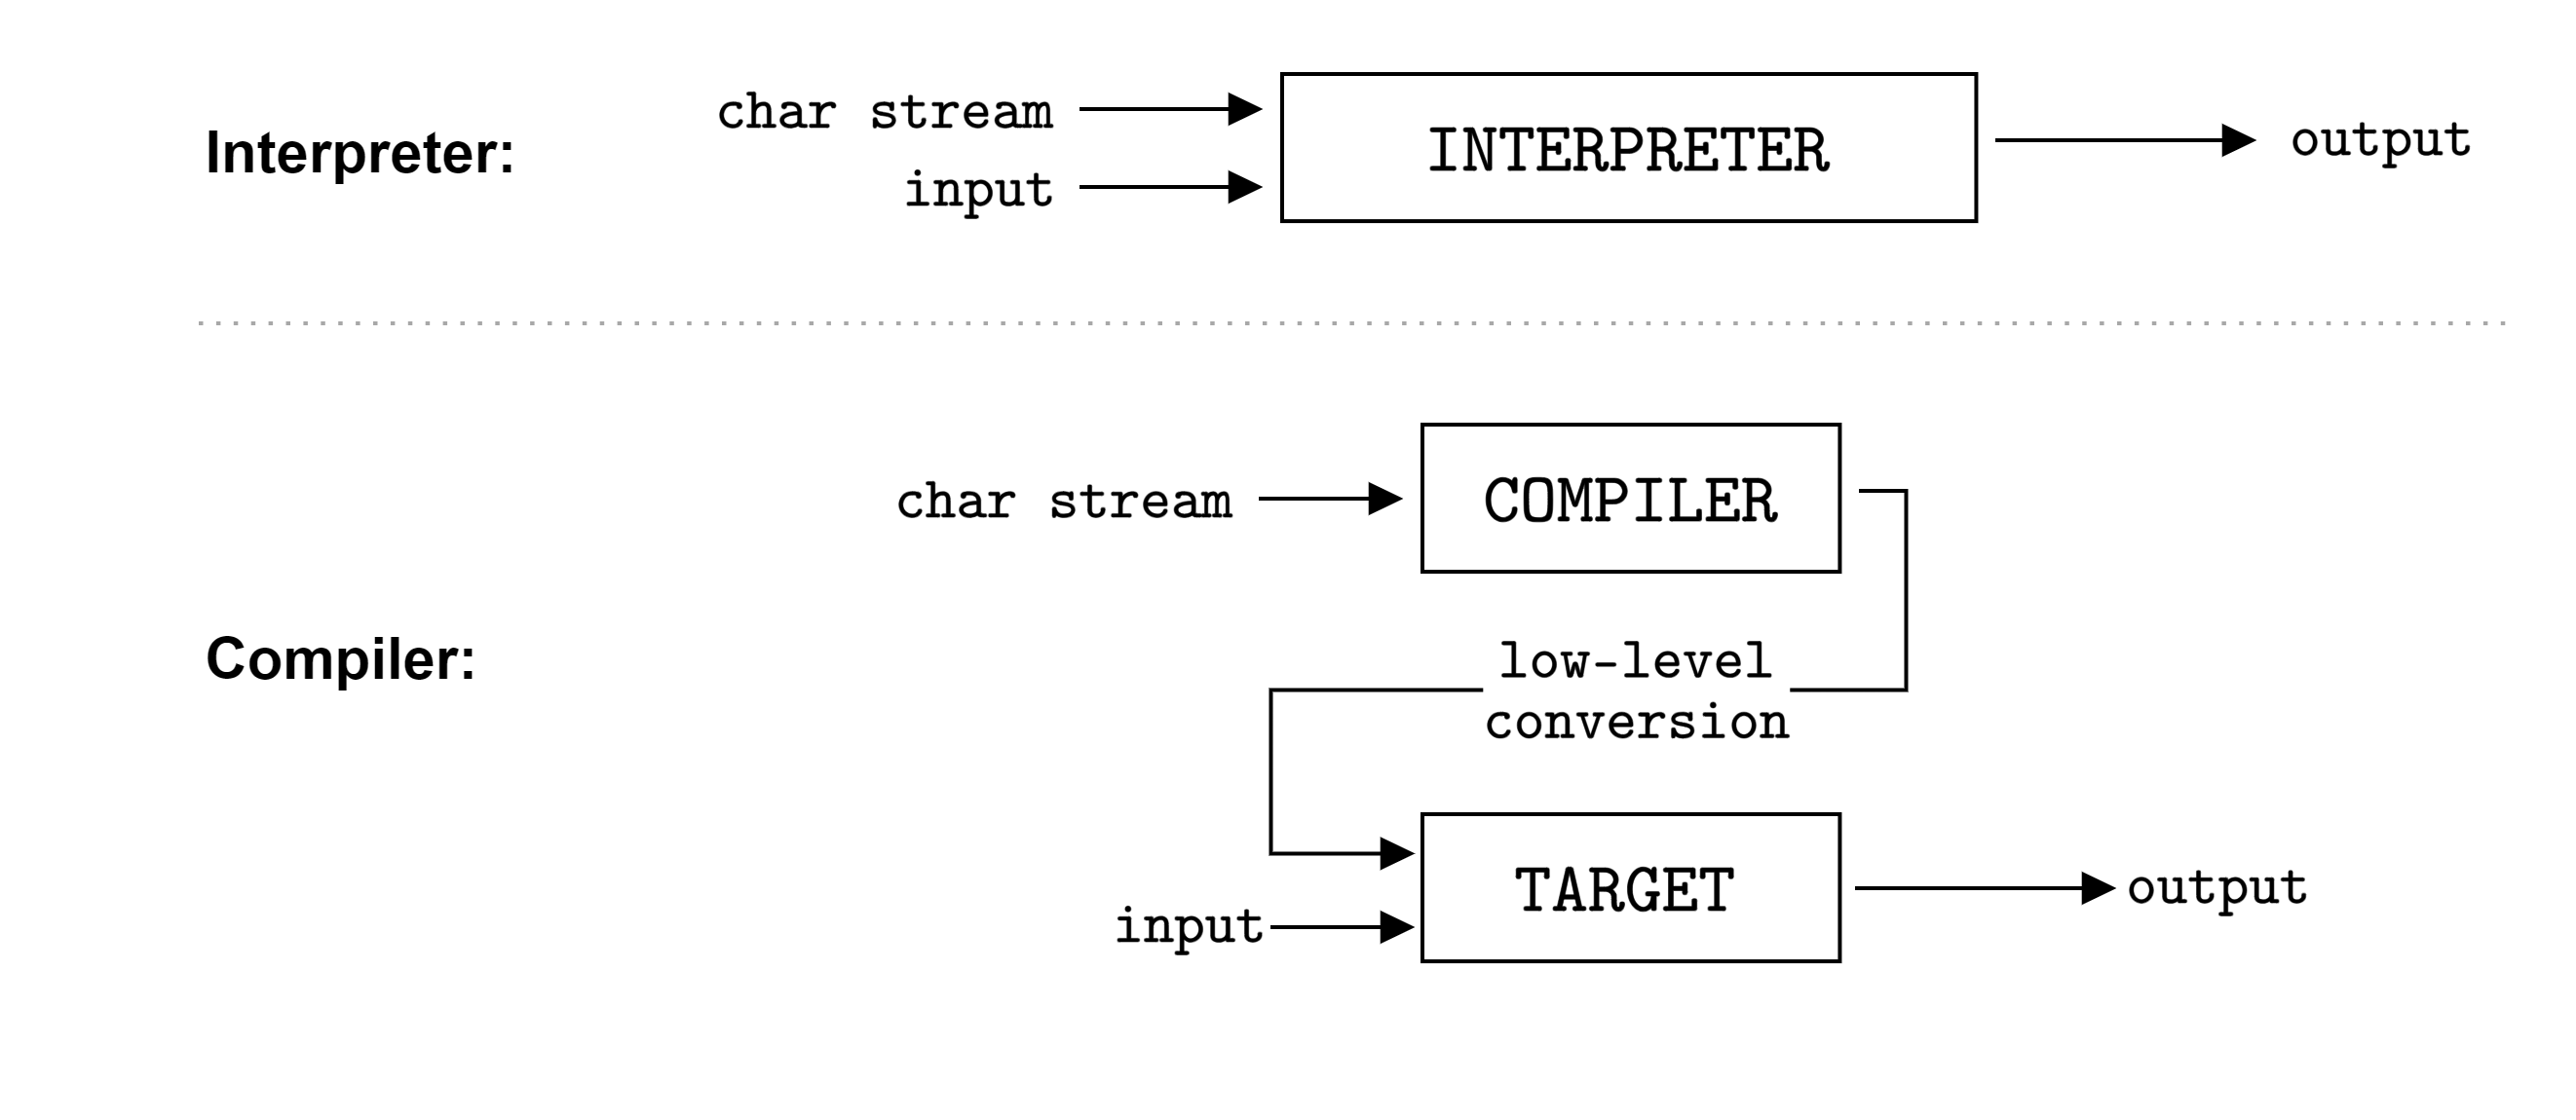
\includegraphics[width=1\textwidth]{Sections/Formal/comp.png}
    \caption{The high-level processes of a compiler and an interpreter.}
\end{figure}

\noindent
The flow of a program through a compiler or interpreter is as follows:
\begin{figure}[h]
    \centering
    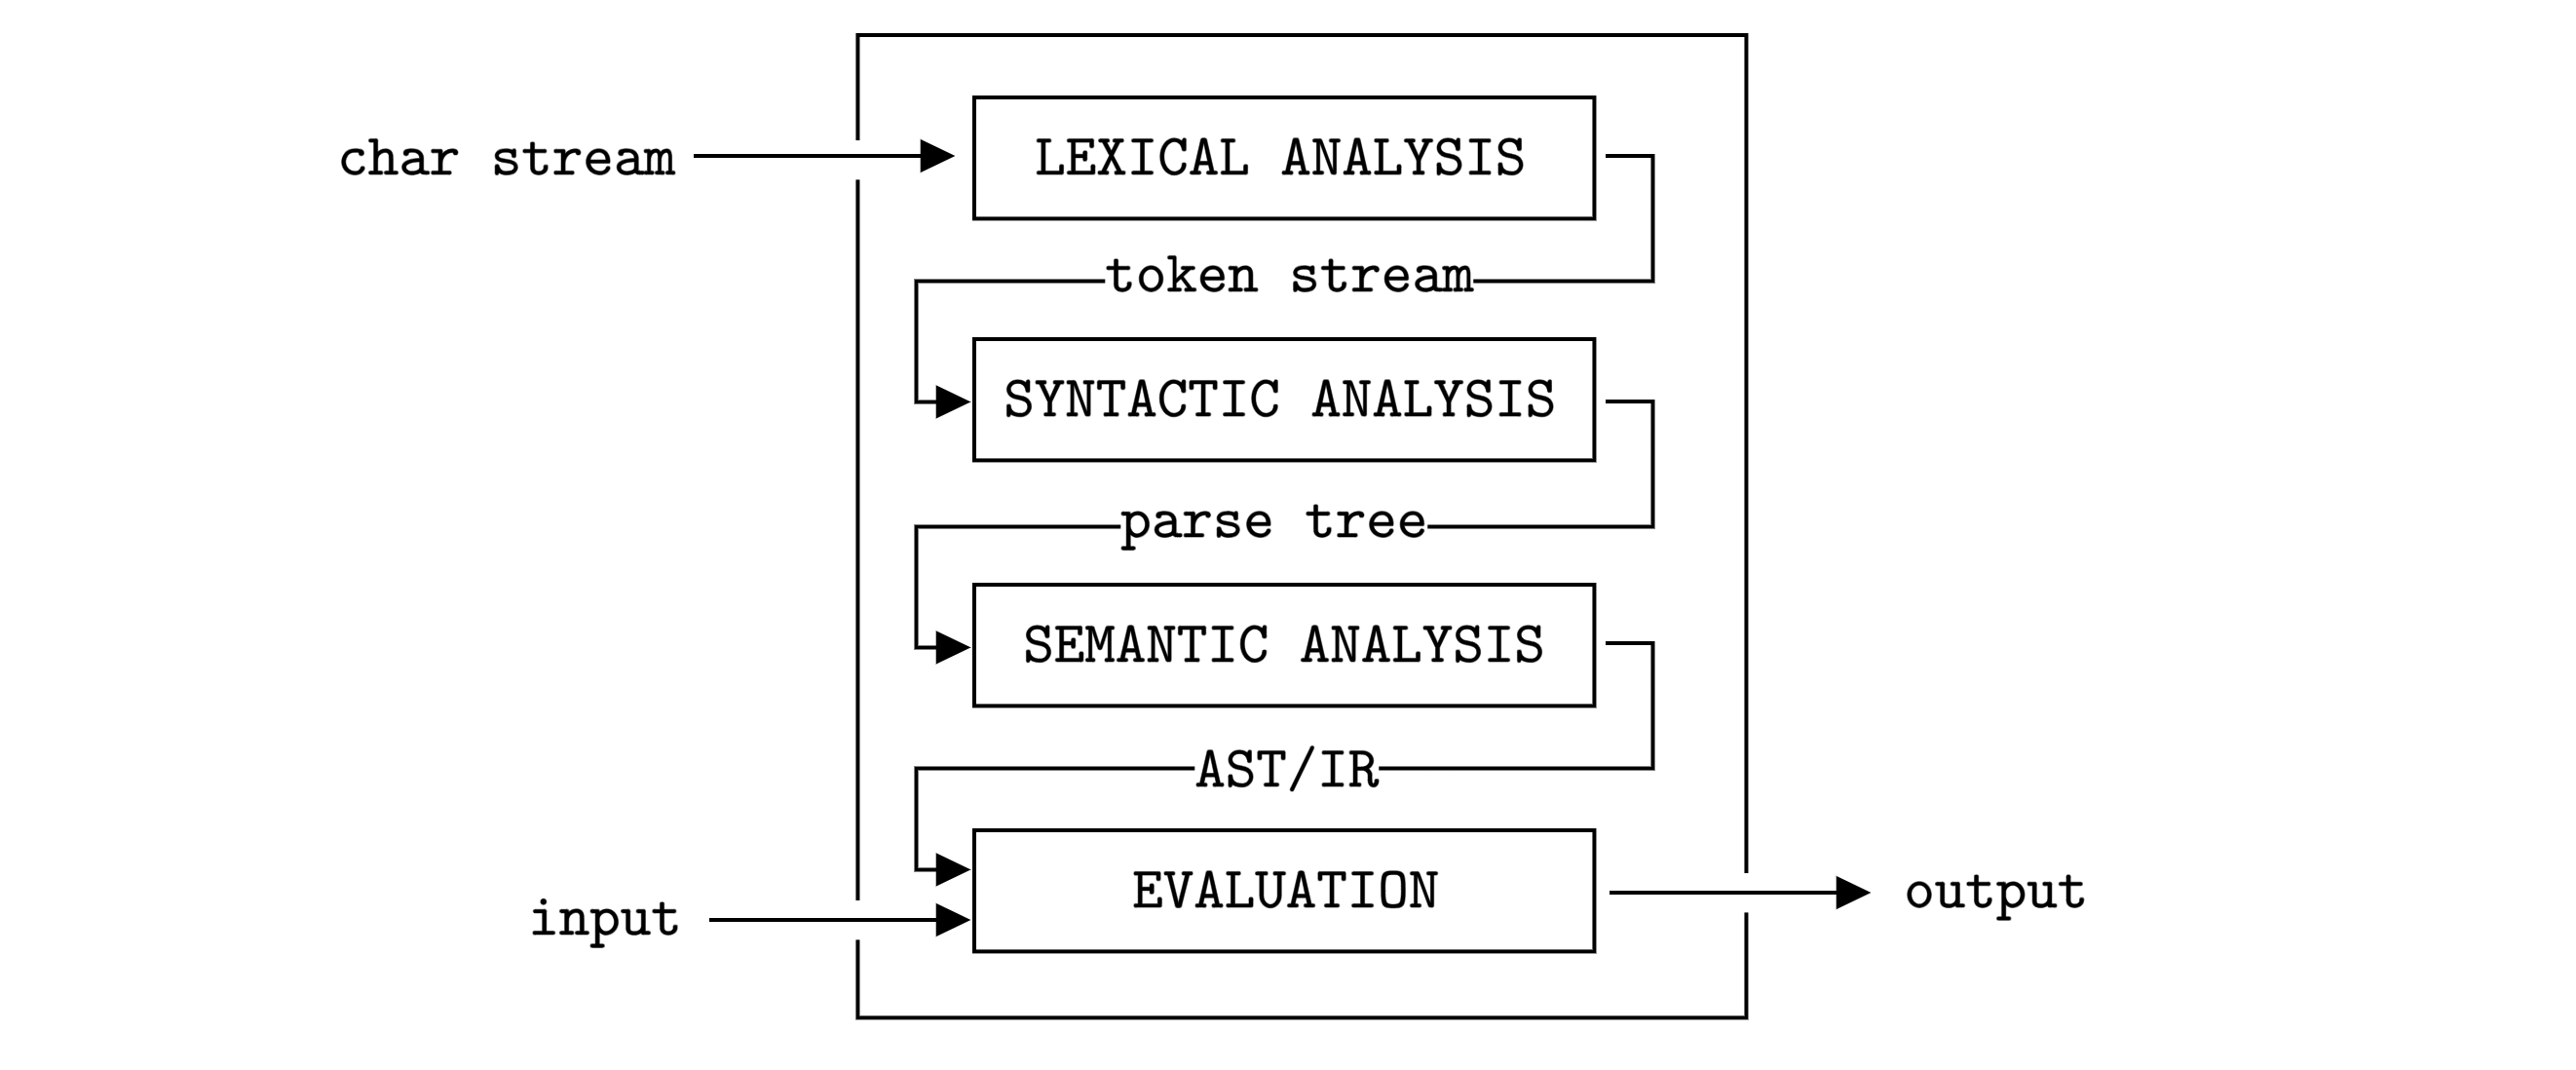
\includegraphics[width=1\textwidth]{Sections/Formal/comp2.png}
    \caption{Stages of program processing: A character stream undergoes lexical, syntactic, and semantic analysis, transforming into an AST or IR before evaluation. Interpreters execute the AST/IR directly, while compilers translate it into machine code.}
\end{figure}

\newpage
    
\noindent
\noindent
To formally layout our language, we use the \textbf{Backus-Naur Form (BNF)} notation. But before we 
do so, we gain some intuition by breaking down an english sentence from its \textbf{terminal symbols}, to its \textbf{non-terminal symbols}. Recall these terms from the pre-requisite section (\ref{def:non-terminal-terminal}).\\

\begin{figure}[h]
    \centering
    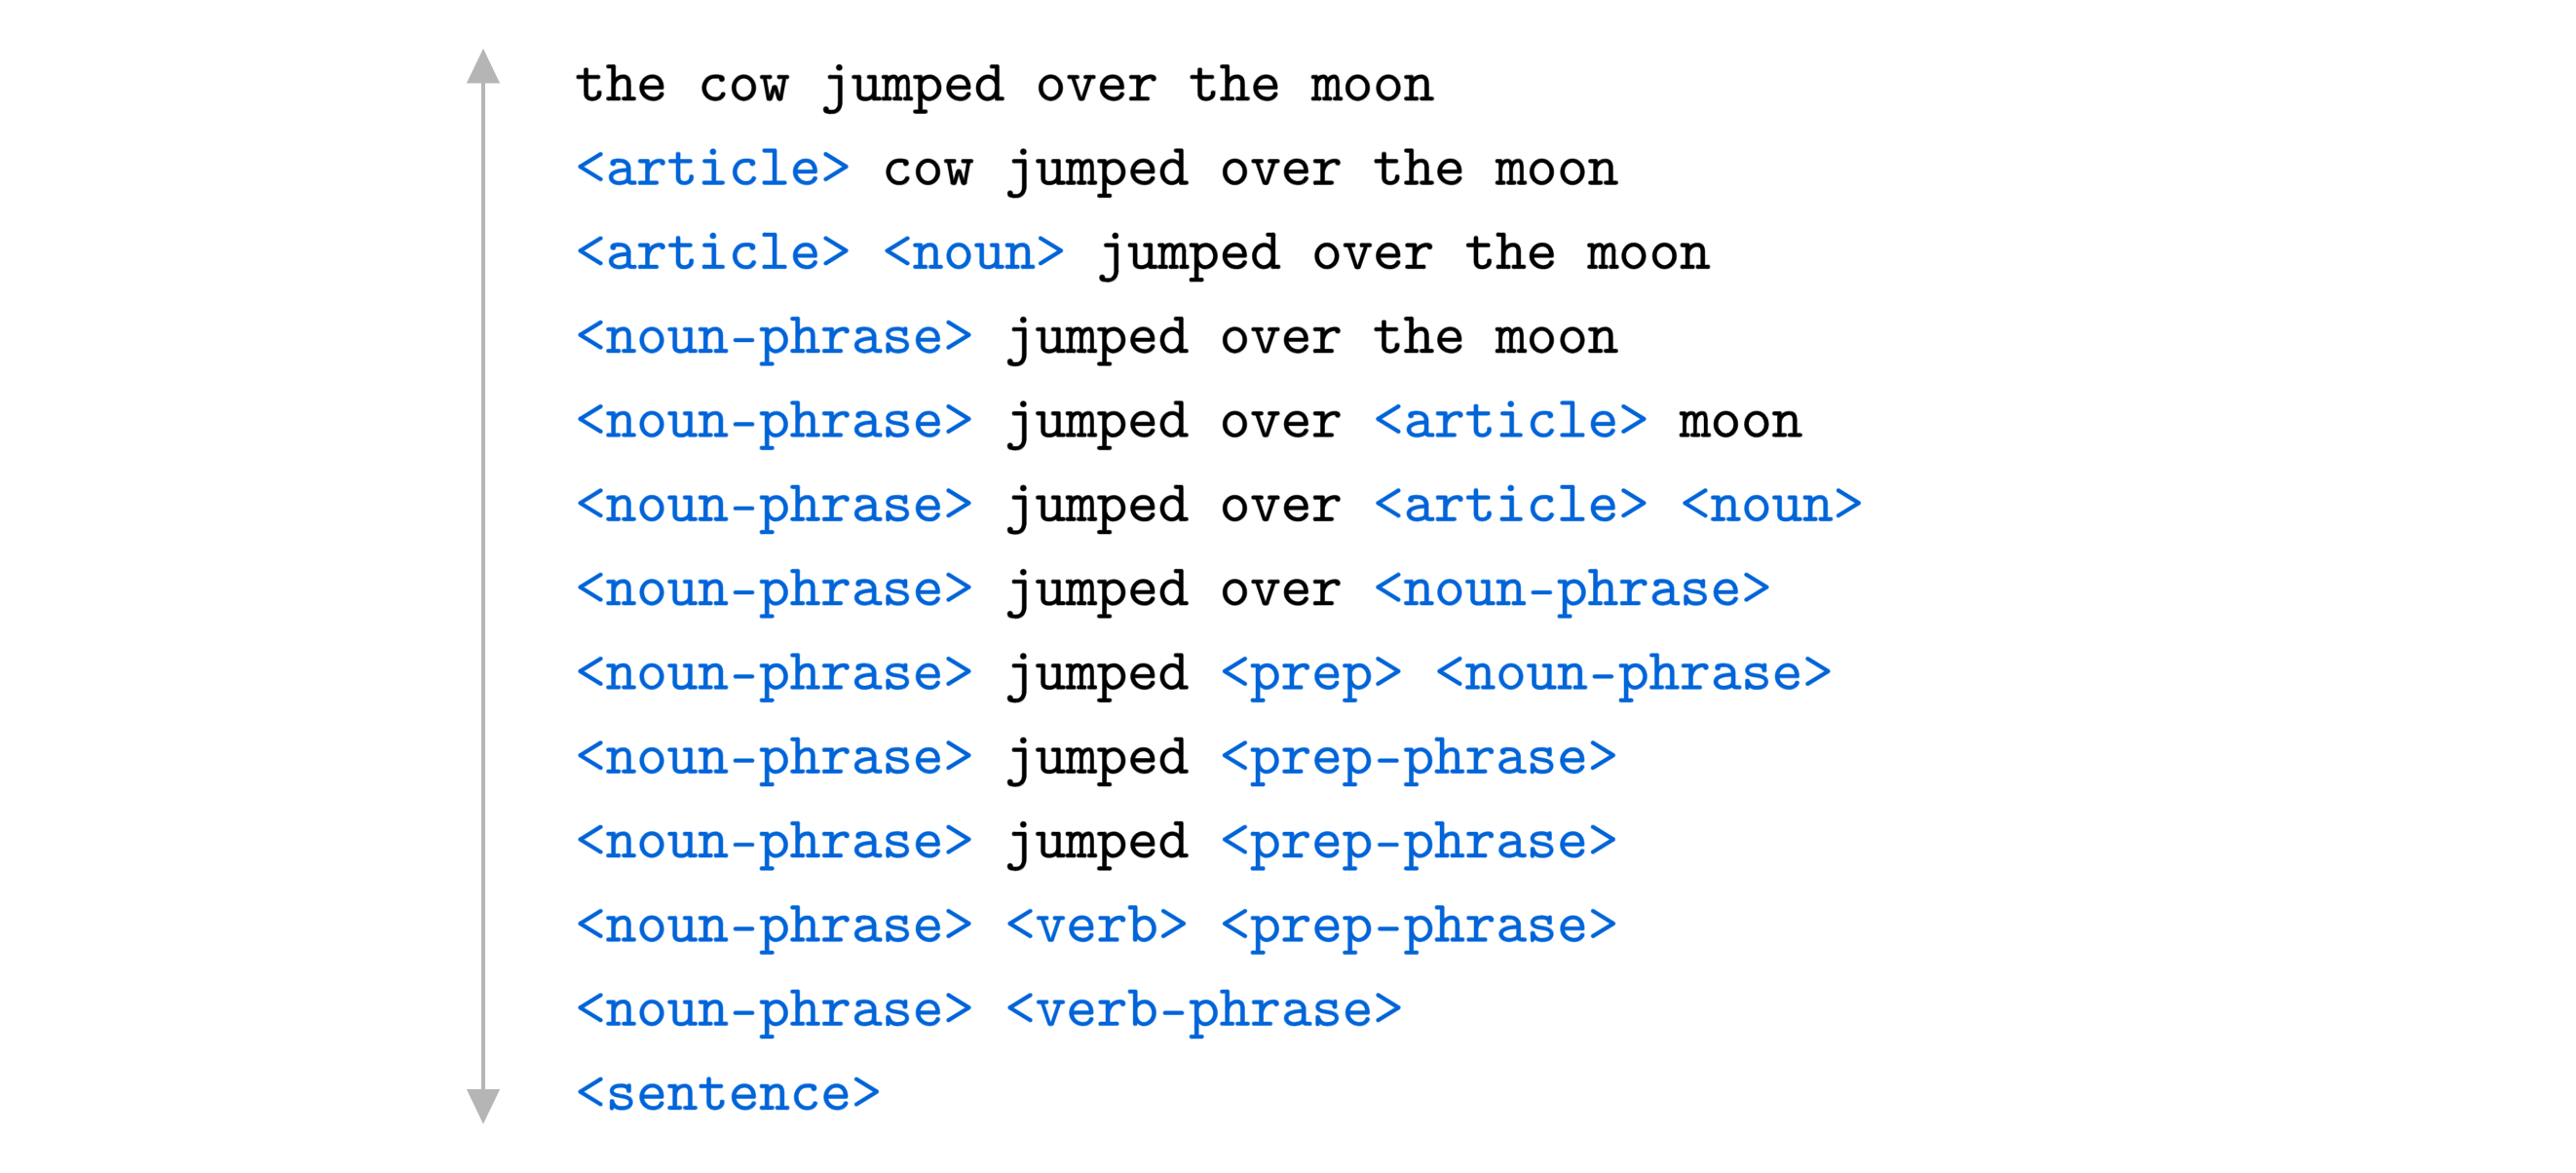
\includegraphics[width=1\textwidth]{Sections/Formal/derivation.png}
    \caption{The sentence ``The cow jumped over the moon.'' broken down into terminal and non-terminal symbols. This is a derivation showing how the sentence is built up from the start symbol of a \texttt{<sentence>}.}
\end{figure}

\noindent
From which the above can be represented in a tree structure:
\begin{figure}[h]
    \centering
    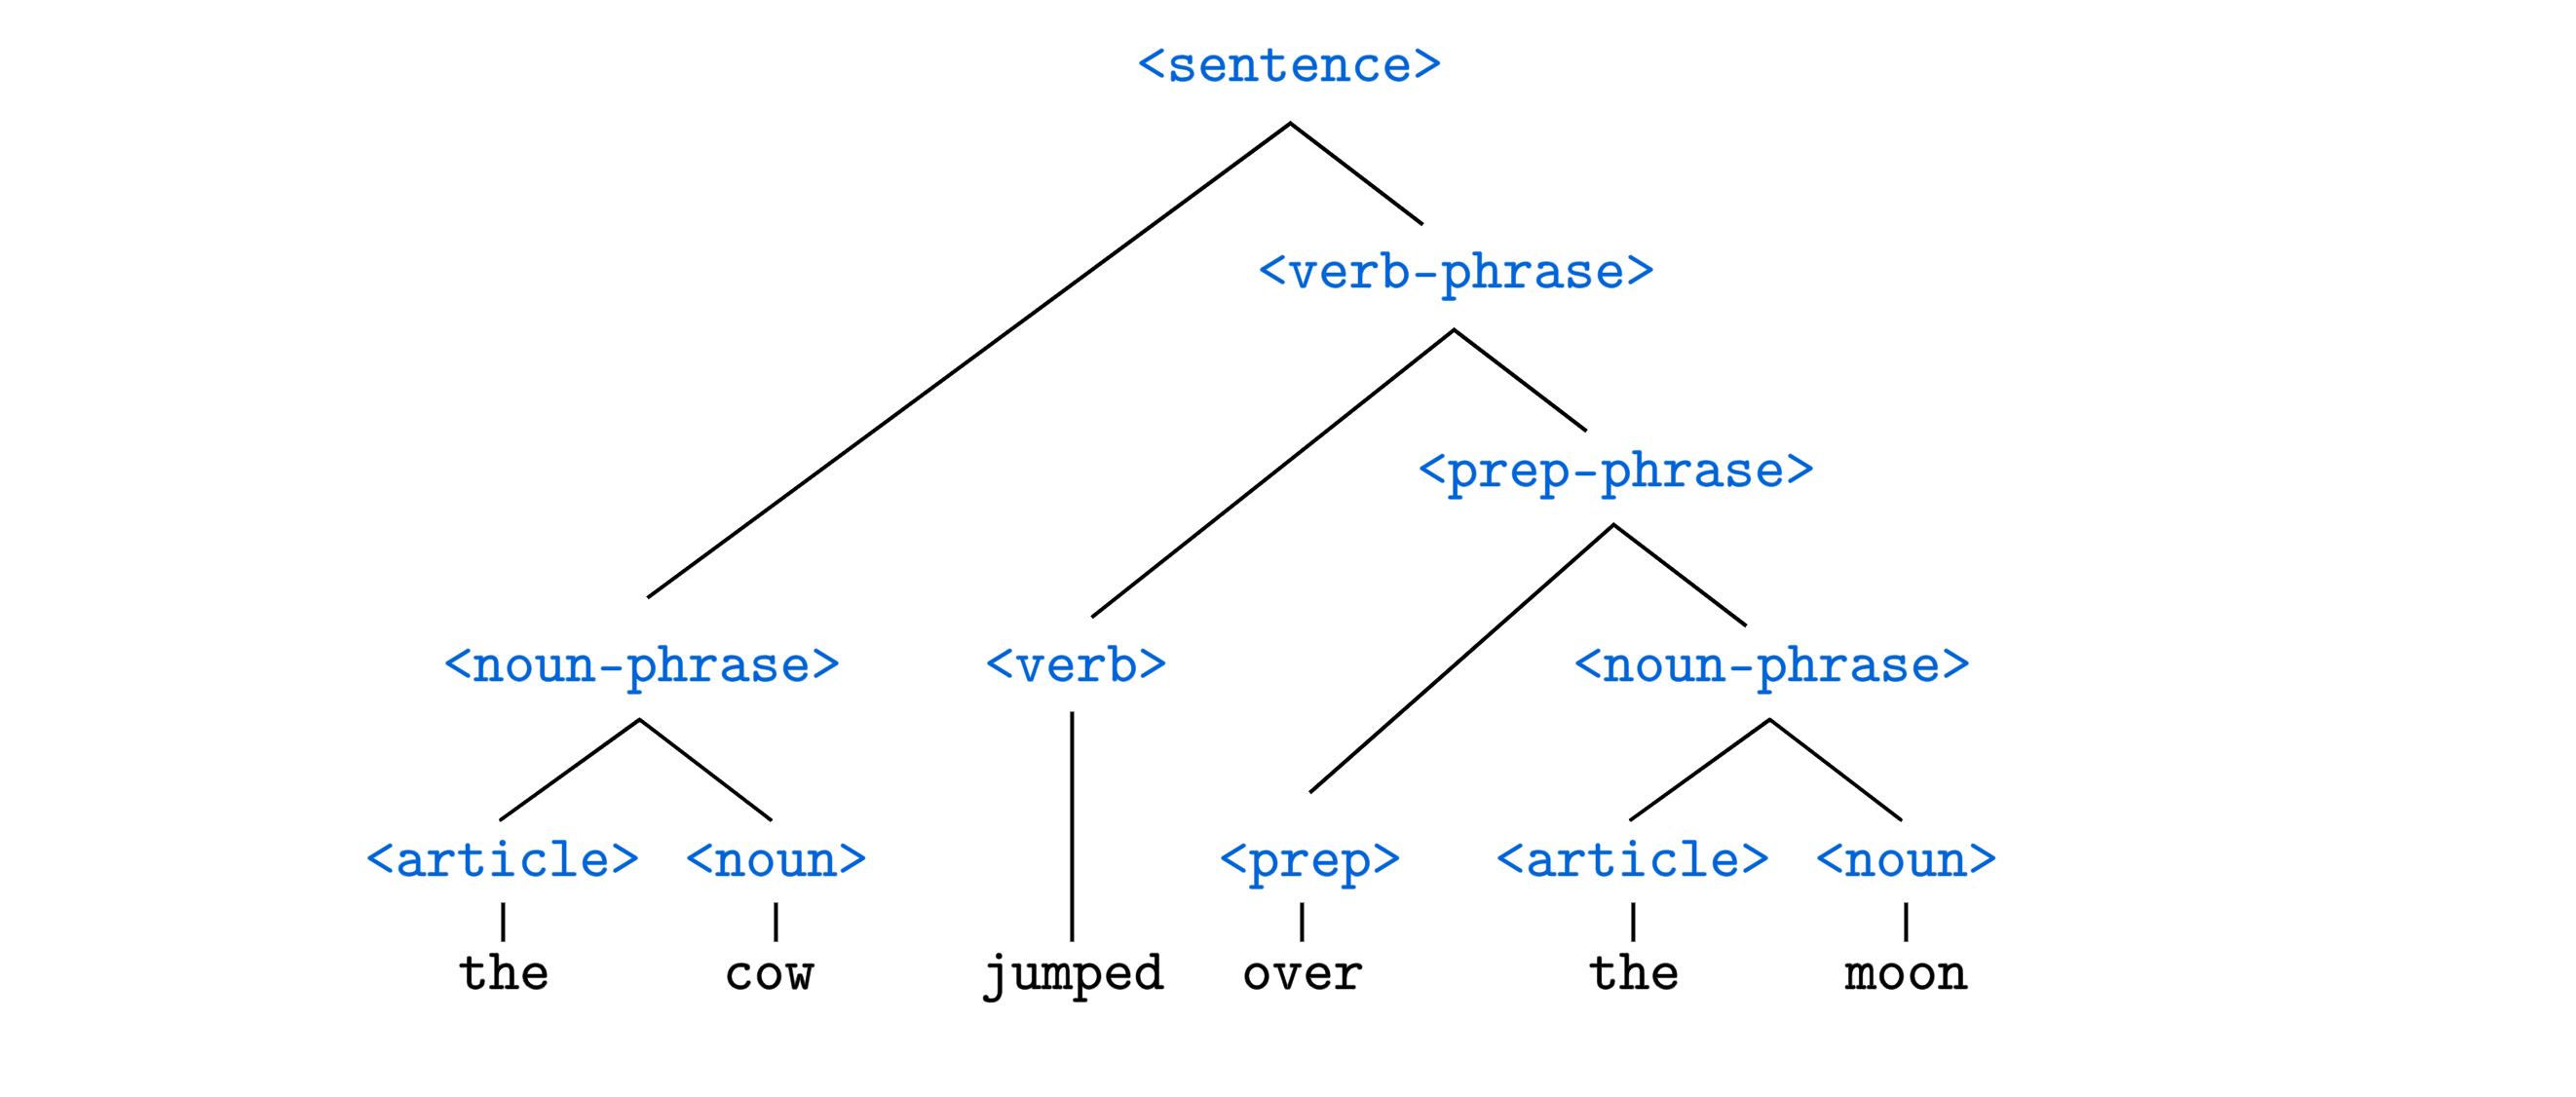
\includegraphics[width=1\textwidth]{Sections/Formal/tree.png}
    \caption{The sentence ``The cow jumped over the moon,'' represented as a \textbf{parse-tree}.}
\end{figure}

\newpage

\noindent
Now if we wanted to state these rules before-hand that a \texttt{<sentence>} is made up of a \texttt{<noun-phrase>} and a \texttt{<verb-phrase>} we can do so as such:

\begin{figure}[h]
    \centering
    
\includegraphics[width=1\textwidth]{Sections/Formal/bnf.png}
    \caption{The rules for the sentence ``The cow jumped over the moon,'' via a thread of production rules (\ref{def:production_rule}). This example illustrates \textbf{Backus-Naur Form (BNF)} notation.}
\end{figure}

\vspace{-1em}
\begin{Def}[Backus-Naur Form (BNF)]

    \textbf{Backus-Naur Form (BNF)} is a formal notation used to define the context. It consists of production rules that specify how symbols in a language can be recursively composed. Each rule follows the form:
    
    \begin{center}
    \texttt{<non-terminal> ::= expression}
    \end{center}
    
    \noindent
    where \texttt{<non-terminal>} represents a syntactic category, and \texttt{expression} consists of terminals, non-terminals, or alternative sequences.
    
    \end{Def}

    \vspace{-.5em}
    \noindent
        Consider a more programmer-like example, assuming we read from left-to-right:

        \begin{figure}[h]
            \centering
            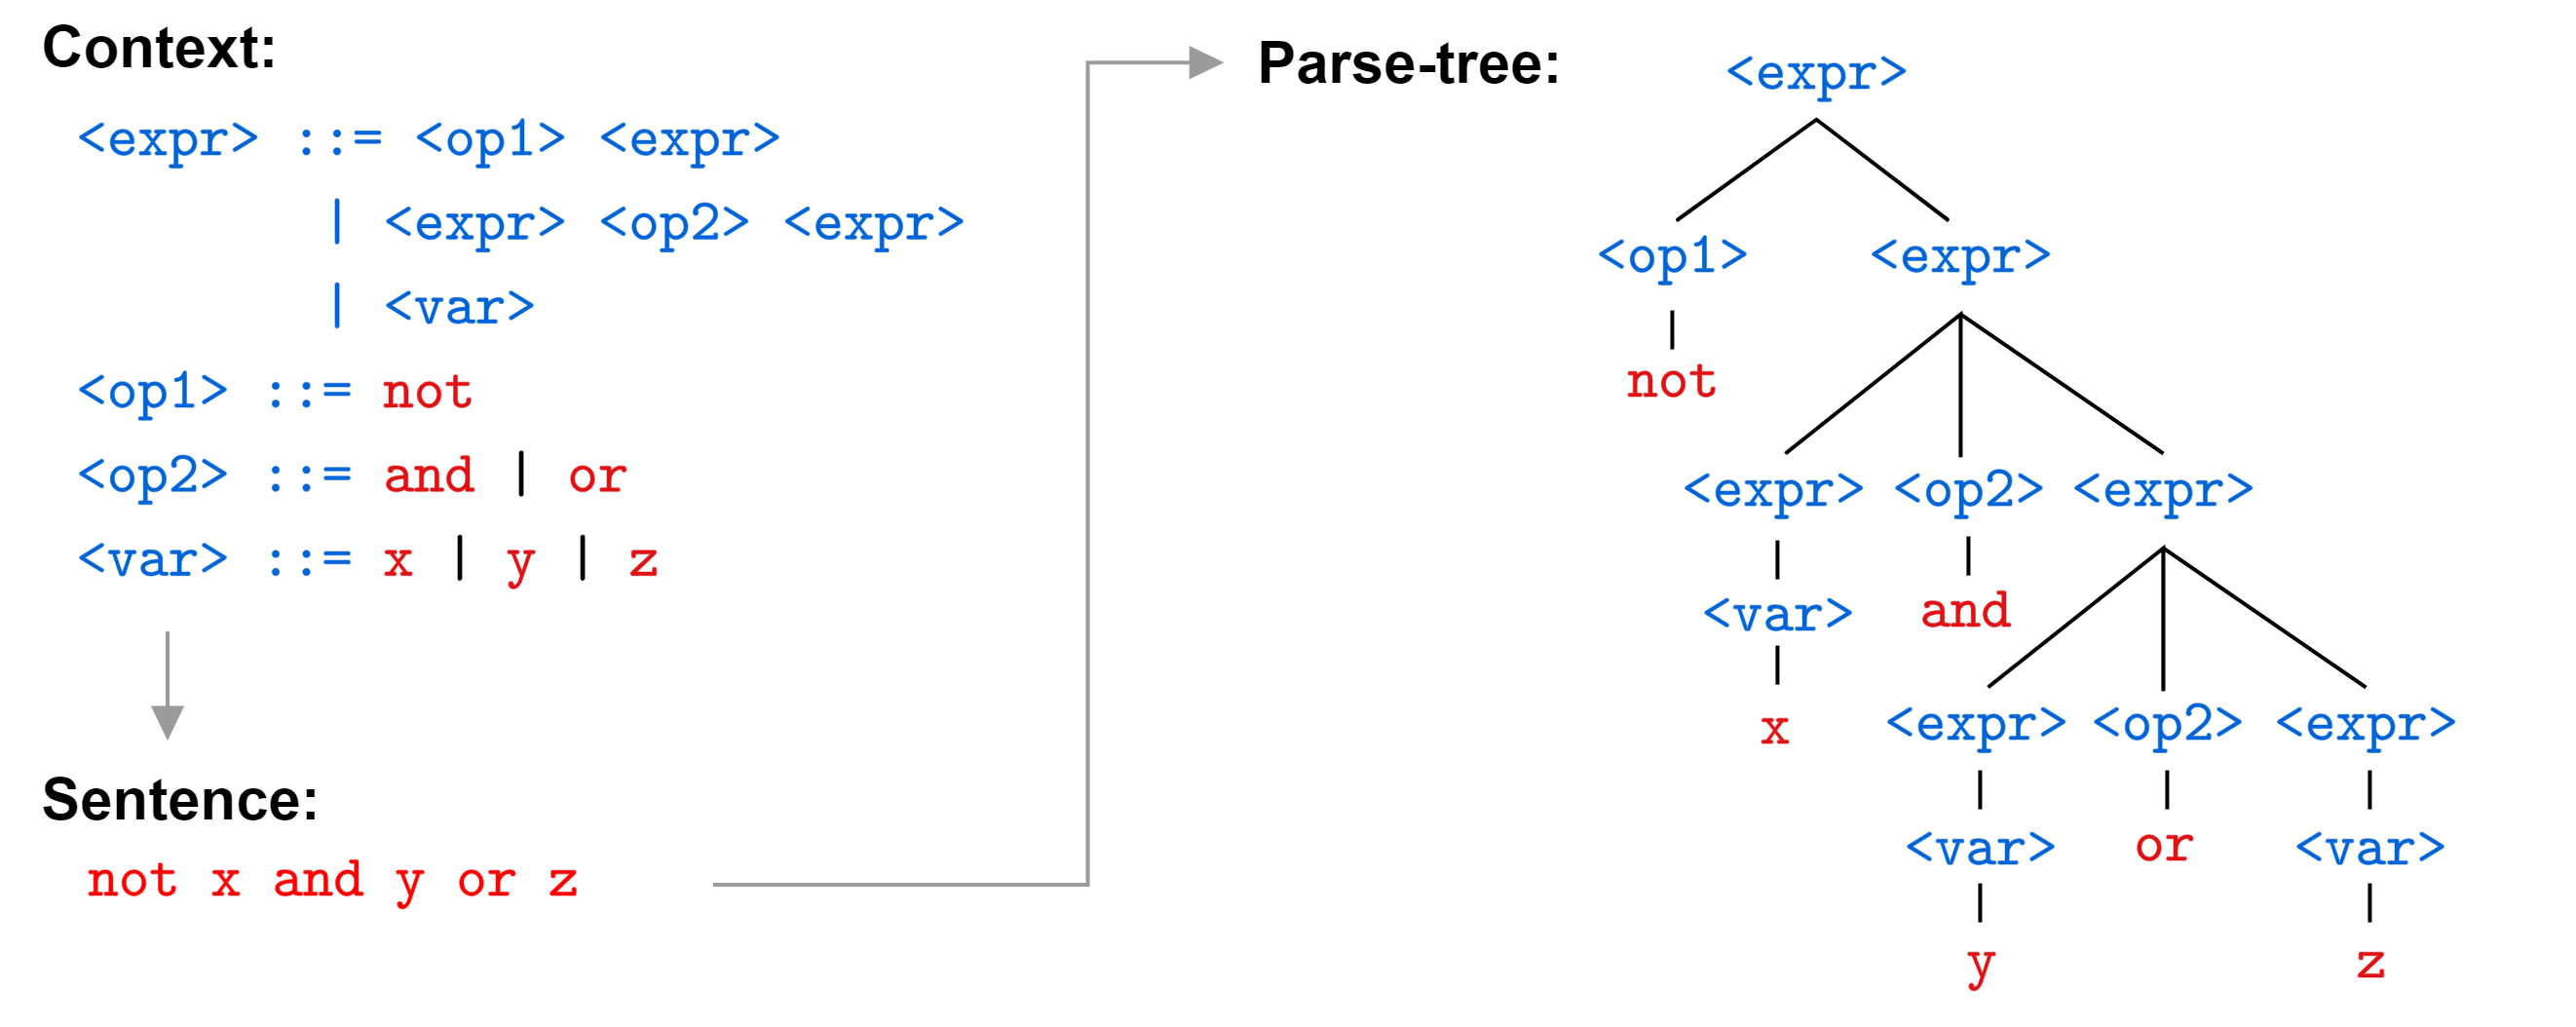
\includegraphics[width=1\textwidth]{Sections/Formal/bnf2.png}
            \caption{A simple language, consisting of \texttt{and} and \texttt{or} operations.}
            \label{fig:bnf2}
        \end{figure}

\newpage

\noindent
The process of taking non-terminal symbols and replacing them with terminal symbols is called a \textbf{leftmost derivation}.
\begin{Def}[Leftmost Derivation]

    A \textbf{leftmost derivation} is a sequence of sentential forms in which, at each step, the \textbf{leftmost} non-terminal symbol is replaced according to a production rule. This process continues until the entire string consists only of terminal symbols.
    
\end{Def}
    
\subsection{Ambiguity in Grammars}

In natural language we have cases where what we say can be ambiguous. For example,
\begin{center}
    \textit
    {``The duck is ready for the dinner table.''}
\end{center}

\noindent
Natural questions may arise:
\begin{itemize}
    \item Was the duck ready to be eaten?
    \item Was the duck a servant preparing the table for dinner?
    \item Was the duck a wrestler, ready to body-slam a constituent?
\end{itemize}
\noindent
For instance, let's clean up the previous sentence, avoiding any, and all ambiguity:
\begin{center}
    \textit
    {``The duck is ready \textbf{to body slam} the dinner table.''}
\end{center}
\noindent
Now Consider the previous example of \texttt{and or not} operations from Figure (\ref{fig:bnf2}):
\begin{figure}[h]
    \centering
    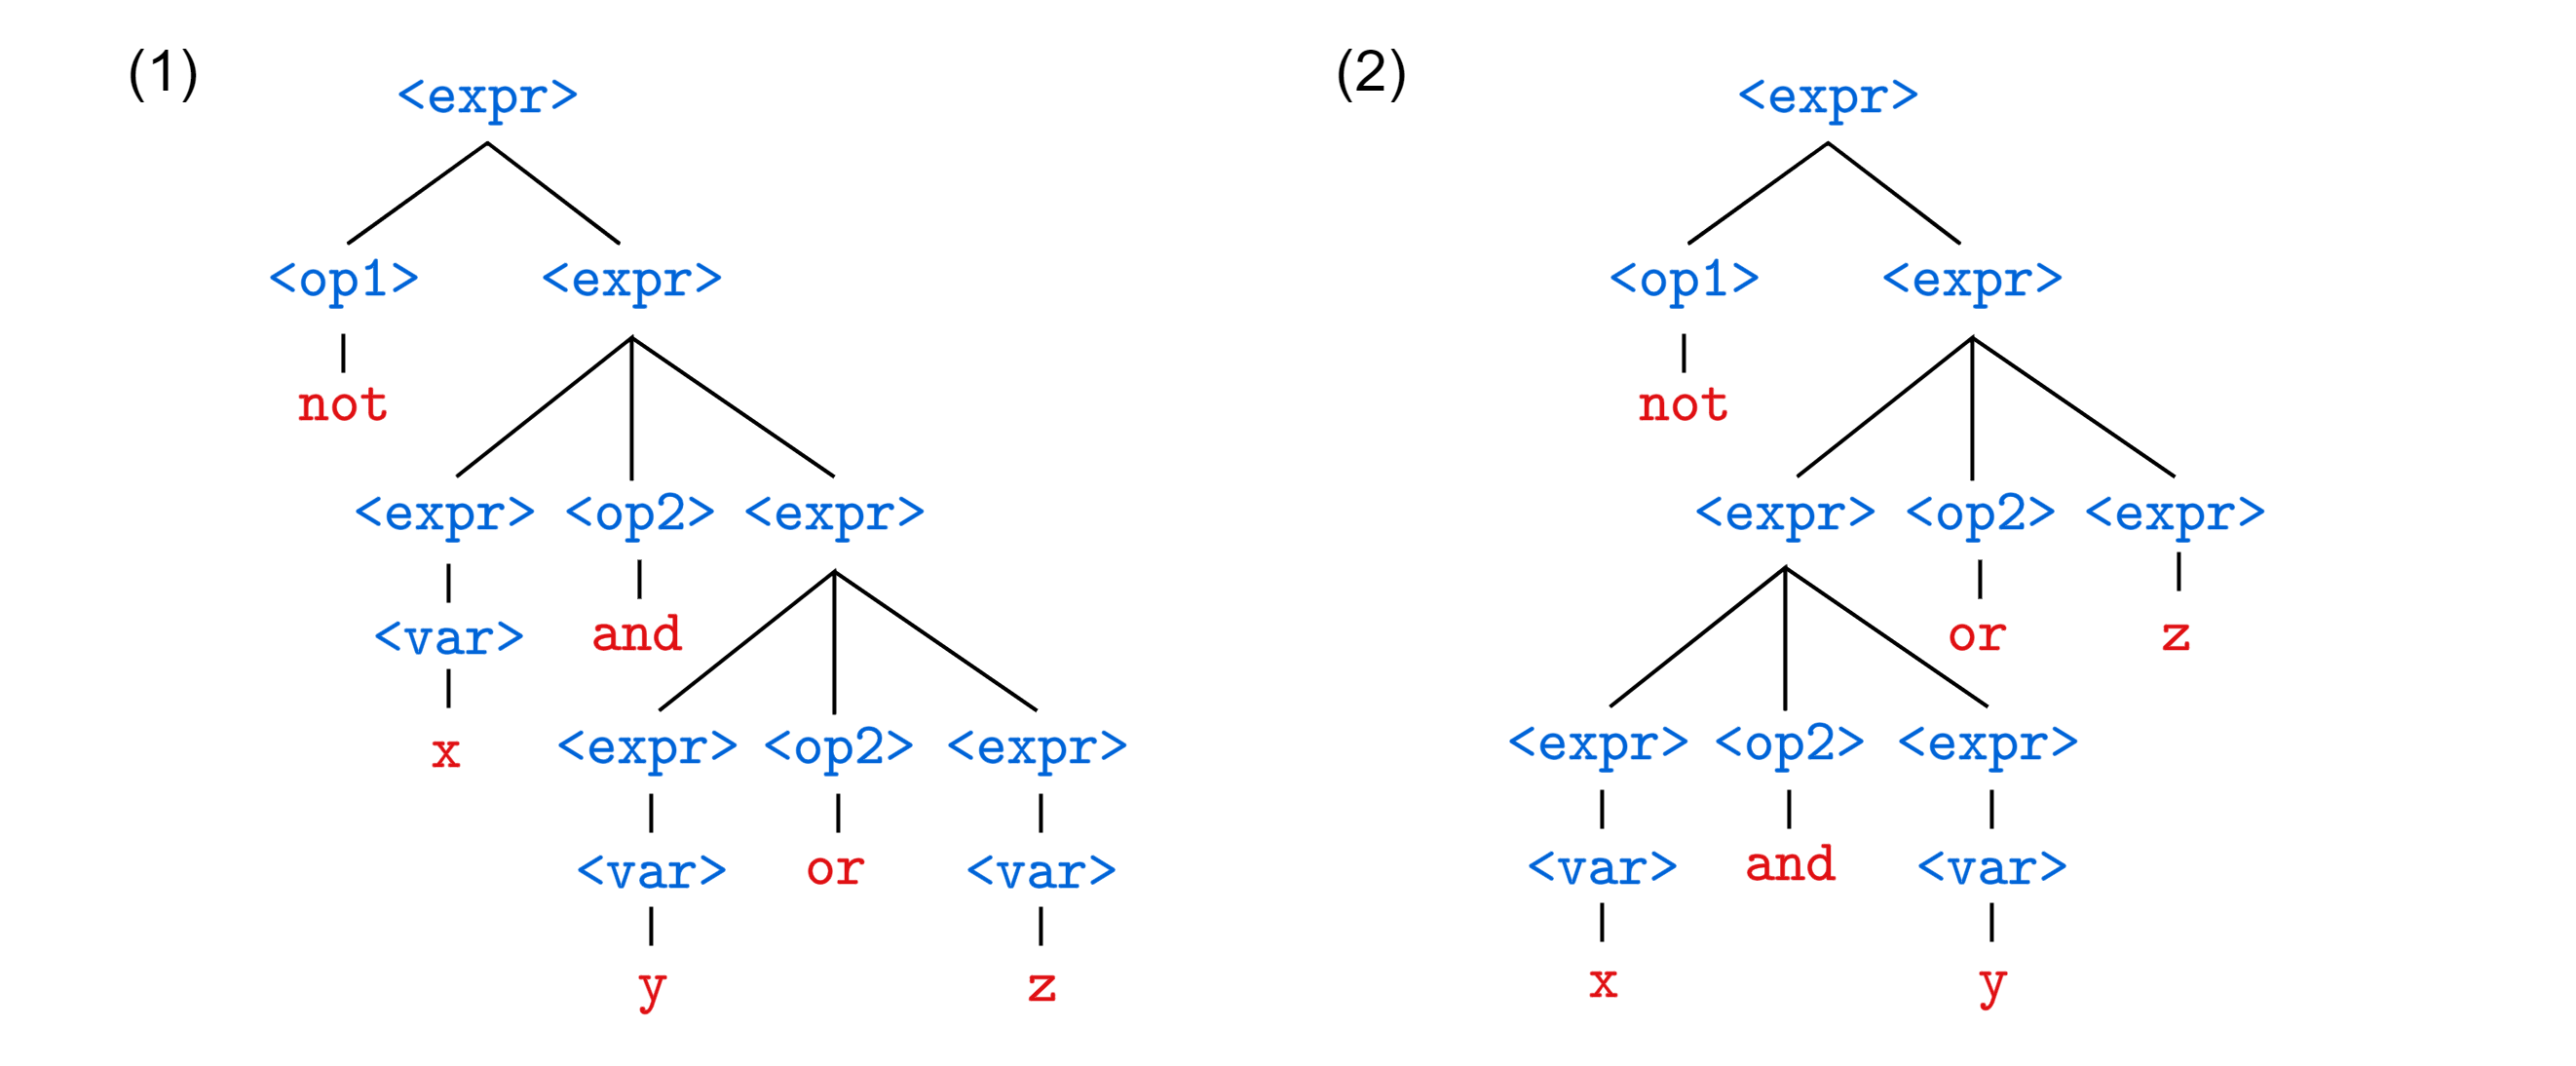
\includegraphics[width=1\textwidth]{Sections/Formal/amb.png}
    \caption{Two possible parse-tree derivations based off of Figure (\ref{fig:bnf2}). (1) Shows our previous intention, while (2) shows a different interpretation, if parsing order was not specified.}
    \label{fig:amb}
\end{figure}

\newpage

\noindent
In Figure (\ref{fig:amb}), (1) shows, \texttt{\textcolor{Wine}{not x and (y or z)}} while (2) shows, \texttt{\textcolor{Wine}{not (x and y) or z}}. This ambiguity can cause issues; for example, 
$x=y=False$, $z=True$, yields different results for (1) and (2). \\

\begin{Def}[Ambiguity in BNF Grammar]

    A \textbf{BNF grammar} is \textbf{ambiguous} if there exists a sentence with multiple valid parse-trees.
\end{Def}
    
\noindent
These, small pieces of ambiguity can crop up anywhere. Consider the following example:
\begin{figure}[h]
    \centering
    
\includegraphics[width=1\textwidth]{Sections/Formal/amb2.png}
    \caption{An ambiguous grammar \texttt{if} expressions.}
    \label{fig:amb2}
\end{figure}

\noindent
In Figure (\ref{fig:amb2}) contains sub-cases which can lead to ambiguity. As, ``is it the sub-case or the super-case?'' For 
example, consider:
\begin{center}
    \texttt{\textcolor{Wine}{if x then (if y then z else w)}}\quad and \quad \texttt{\textcolor{Wine}{if x then (if y then z) else w}}
\end{center}

\noindent 
These problems often arise when interpreting expressions at the linear level. On an important note:
\begin{theo}[Ambiguity is Undecidable]
    
    It is impossible to write a generalized program to determine if a given grammar set is ambiguous.
    This requires to finding all possible sentences; \textbf{However}---our grammar is recursive---this would mean generating 
    an infinite number of sentences.
\end{theo}

\noindent
Though we can avoid ambiguity by specifying our operation order:
\begin{Def}[Fixity]

    The \textbf{fixity} of an operator refers to its placement relative to its operands:
    
    \begin{itemize}
        \item \textbf{Prefix}: The operator appears \textit{before} its operand (e.g., $f\ x$, $-x$).
        \item \textbf{Postfix}: The operator appears \textit{after} its operand (e.g., $a!$ for factorial or dereferencing).
        \item \textbf{Infix}: The operator appears \textit{between} two operands (e.g., $a * b$, $a + b$, $a \mod b$).
        \item \textbf{Mixfix}: The operator is interleaved with its operands, appearing in multiple positions (e.g., \texttt{if} $b$ \texttt{then} $x$ \texttt{else} $y$).
    \end{itemize} 
    \end{Def}

\newpage 
\noindent
So by specifying only Prefix or only Postfix operations ambiguity can be avoided:
\begin{Def}[Polish Notation]

    \textbf{Polish Notation} is a notation for arithmetic expressions in which the operator precedes its operands. For example, the polish notation $- / + 2 * 1 - 2 3$ is written as $- (2 + (1 * (- 2) / 3)$.\\
    
    \noindent
    In contrast, \textbf{Reverse Polish Notation} (RPN) places the operator after its operands. For example, Infix: $(3 + 4) * 5$ is $3\ 4 + 5\ *$ in RPN.
\end{Def}

\noindent
However, this is not always practical. Consider \texttt{if} expressions dealt this way:
\begin{figure}[h]
    \centering
    
\includegraphics[width=1\textwidth]{Sections/Formal/amb3.png}
    \caption{An unambiguous grammar for \texttt{if} expressions.}
    \label{fig:amb3}
\end{figure}

\noindent
Likewise, if we decided to enforce parenthesis everywhere, it might be a bit cumbersome:
\begin{figure}[h]
    \centering
    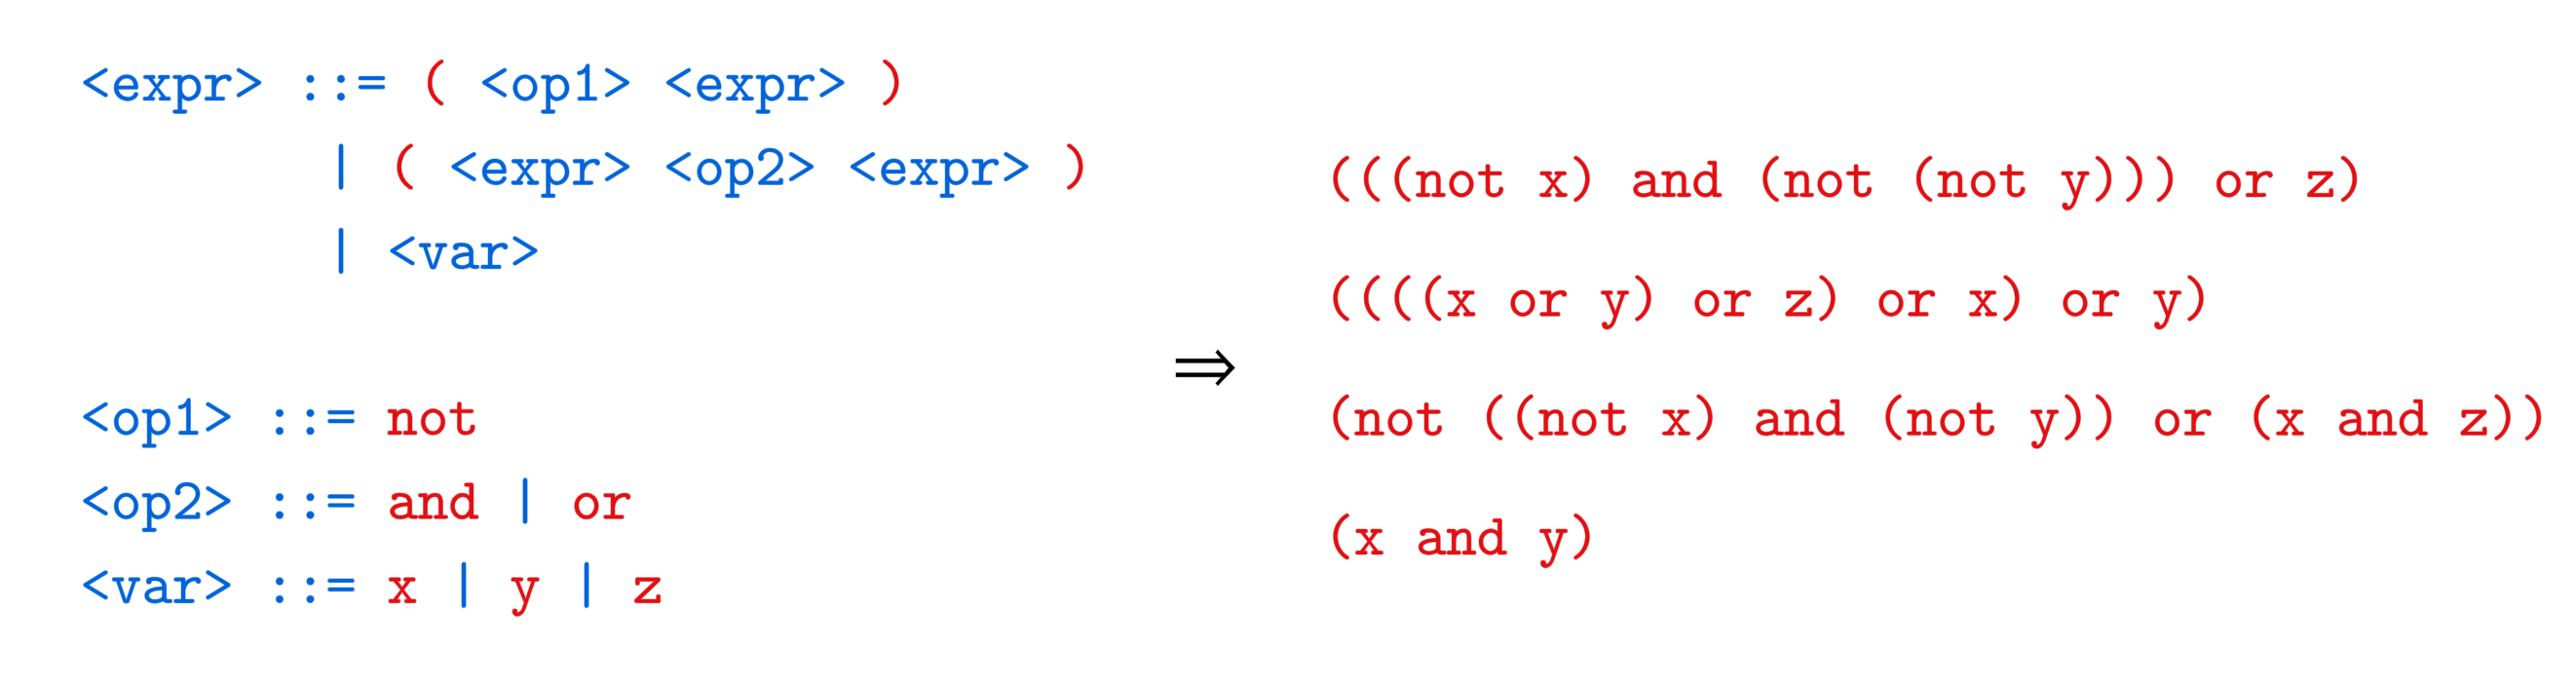
\includegraphics[width=1\textwidth]{Sections/Formal/amb4.png}
    \caption{An unambiguous grammar for \texttt{and or not} expressions, with parenthesis everywhere.}
    \label{fig:amb4}
\end{figure}

\noindent
\begin{theo}[The Ambiguity of Associativity \& Precidence Rules]
    
    \begin{itemize}
        \item \textbf{Associativity}: $a + b + c$ is ambiguous, as it could be $(a + b) + c$ or $a + (b + c)$.
        \item \textbf{Precedence}: $a + b * c + d$ is ambiguous to a computer, as it could be $(a + b) * c + d$.
    \end{itemize}
    \end{theo}
\newpage 

\noindent
We can resolve this by breaking the symmetry of our grammar:
\begin{theo}[Resolving Associativity: Breaking Symmetry]

    The reason for ambiguity often comes symmetry in grammar rules of form:
    \begin{center}
        \texttt{<expr> ::= <expr> <op> <expr>}\\
        \texttt{<op> ::= + | - | ...} \hspace{1.8em} \null
    \end{center}

    \noindent
    This means that the left or right side can be expanded indefinitely. By breaking this symmetry, we can resolve ambiguity:
    \begin{center}
        \texttt{<expr> ::= <var> <op> <expr>}\\
        \texttt{<op> ::= + | - | ...} \hspace{1.3em} \null\\
        \texttt{<var> ::= x | y | z | ...} \hspace{-.3em} \null
    \end{center}
    \noindent
    In the above we fixed the left side to be a \texttt{<var>} and the right side to be an \texttt{<expr>}.
    This makes our expression \textbf{right-associative}. Vice-versa, if we fixed the right side, it would be \textbf{left-associative}.
\end{theo}

\begin{theo}[Resolving Precedence: Factor Out Higher Precedences]

    Precedence issues arise when operations reside on the same level. For instance,
        
    \vspace{-1em}
        \begin{align*}
            \texttt{<expr>} &\texttt{::= <expr> + <expr> | <expr> * <expr>}
        \end{align*}

    \noindent
    Here, it's unclear whether \texttt{+} or \texttt{-} should be evaluated first. By factoring out higher precedence operations, we can resolve this, 
    as, \underline{\textbf{terms deeper in the parse tree are evaluated first}}:
    \begin{align*}
        \texttt{<expr>} &\texttt{::= <expr> + <term> | <term> }\\
        \texttt{<term>} &\texttt{::= <term> * <var> | <var>}\\
        \texttt{<var>} &\texttt{::= x | y | z | ...}
    \end{align*}

    \vspace{-1em}
    \noindent
    Here, \texttt{*} has higher precedence than \texttt{+}, as it's deeper in the parse tree. To handle 
    \textbf{parentheses}, we can introduce another factor:
    \begin{align*}
        \texttt{<expr>} &\texttt{::= <expr> + <term> | <term> }\\
        \texttt{<term>} &\texttt{::= <term> * <pars> | <pars>}\\
        \texttt{<pars>} &\texttt{::= var | ( <expr> )}\\
        \texttt{<var>} &\texttt{::= x | y | z | ...}
    \end{align*}
    \noindent
    Intuitively, in expressions like \texttt{(a + b) * c}, we want to treat \texttt{(a + b)} as a single unit/\textit{variable}. \textbf{Note},
    the parentheses are tokens surrounding the non-terminal \texttt{<expr>}.
\end{theo}

\newpage 

\noindent
Now consider the \texttt{and or not} expressions from Figure (\ref{fig:bnf2}) resolving the associative ambiguity:

\begin{figure}[h]
    \centering
    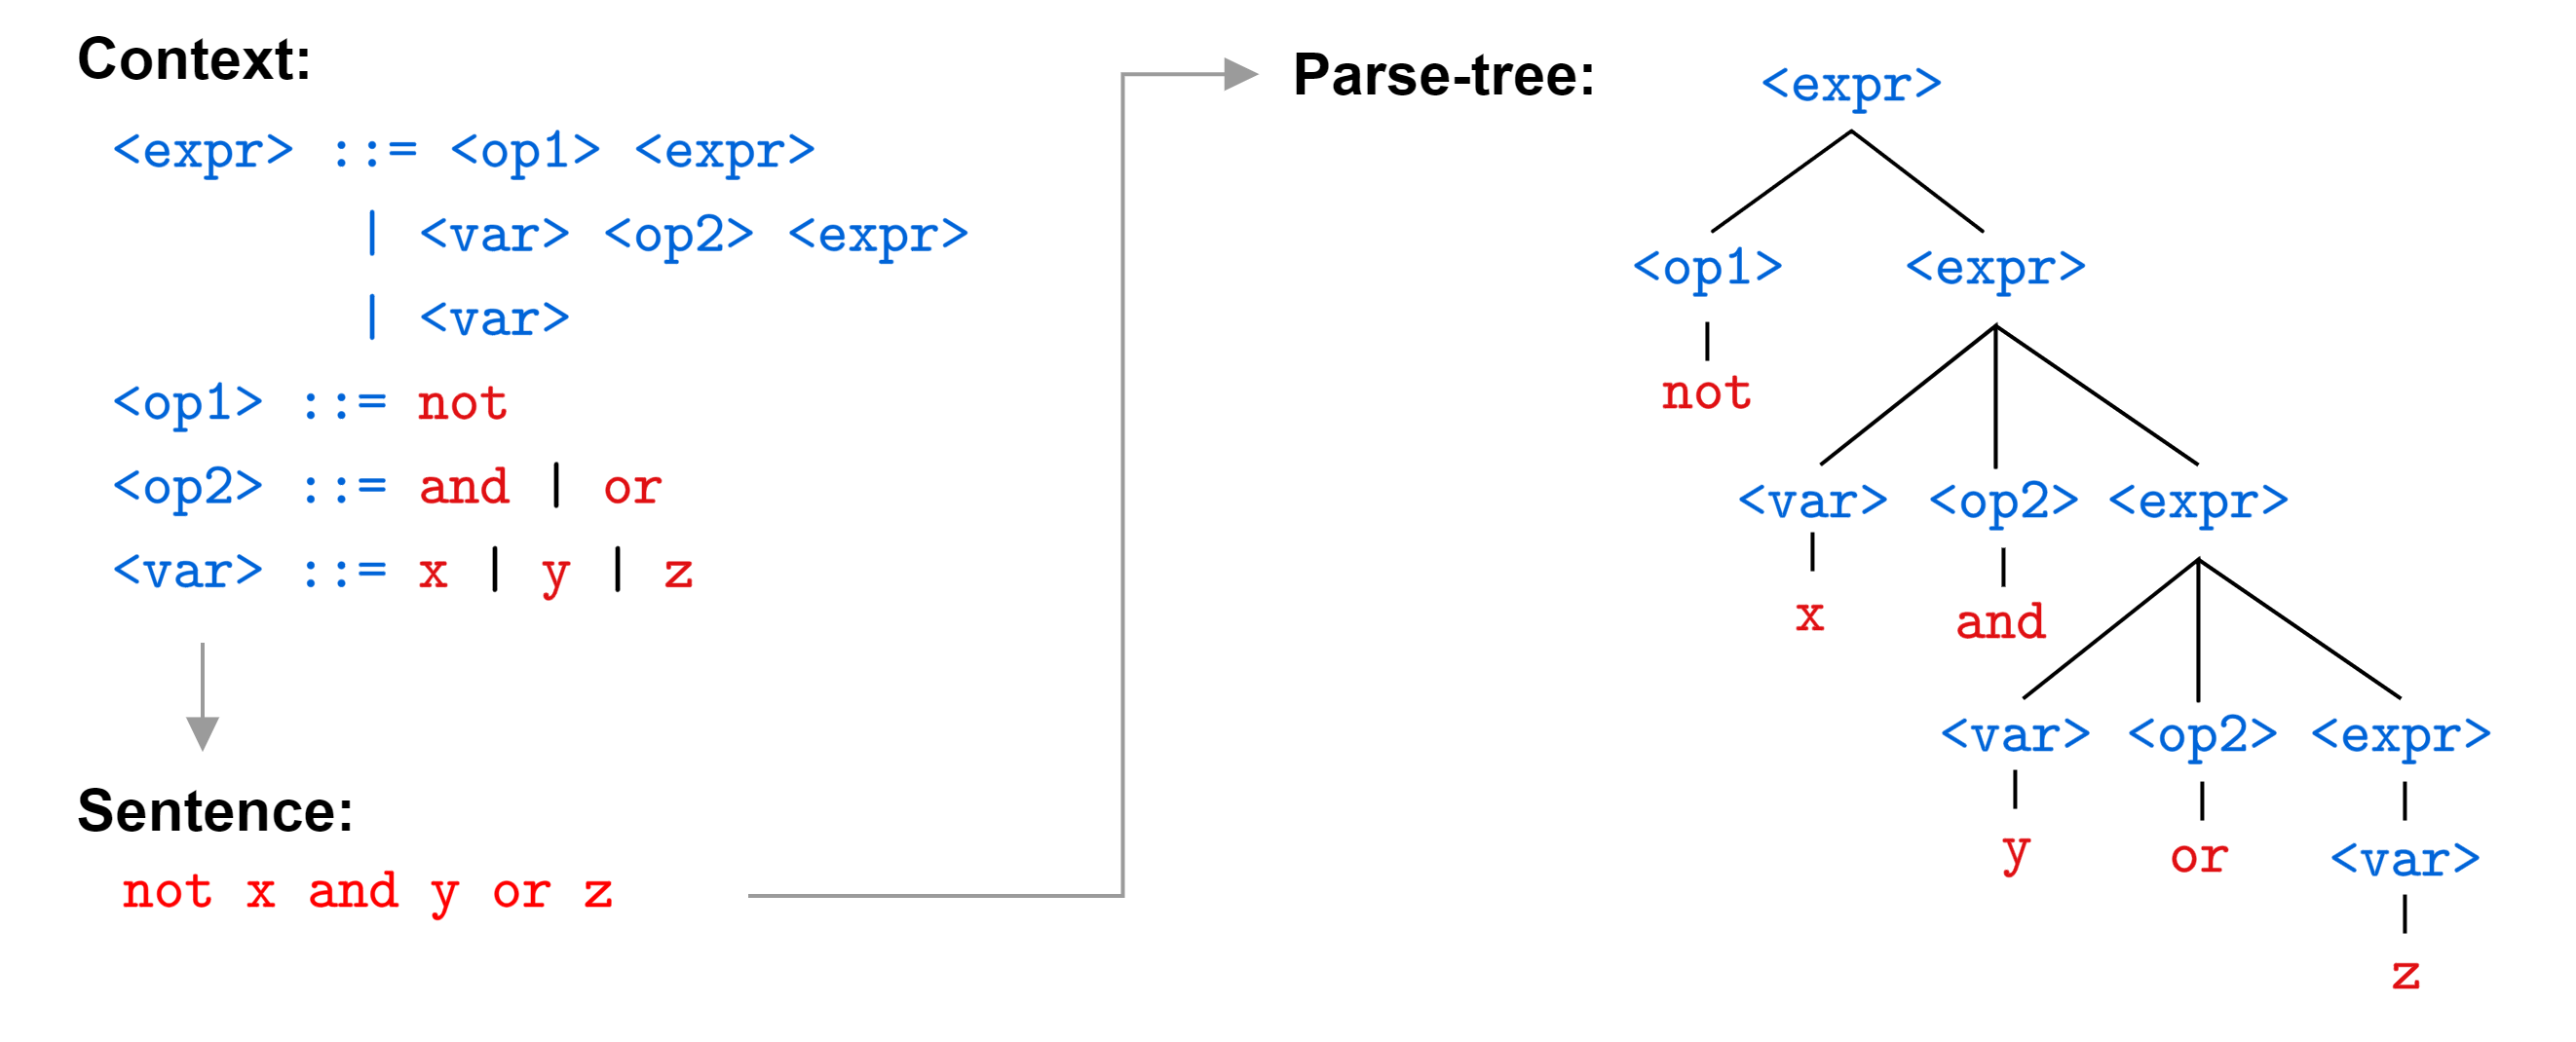
\includegraphics[width=1\textwidth]{Sections/Formal/amb5.png}
    \caption{An unambiguous grammar for \texttt{and or not} expressions, by breaking symmetry.}
    \label{fig:amb5}
\end{figure}

\noindent
Now we put all the rules together:
\begin{figure}[h]
    \centering
    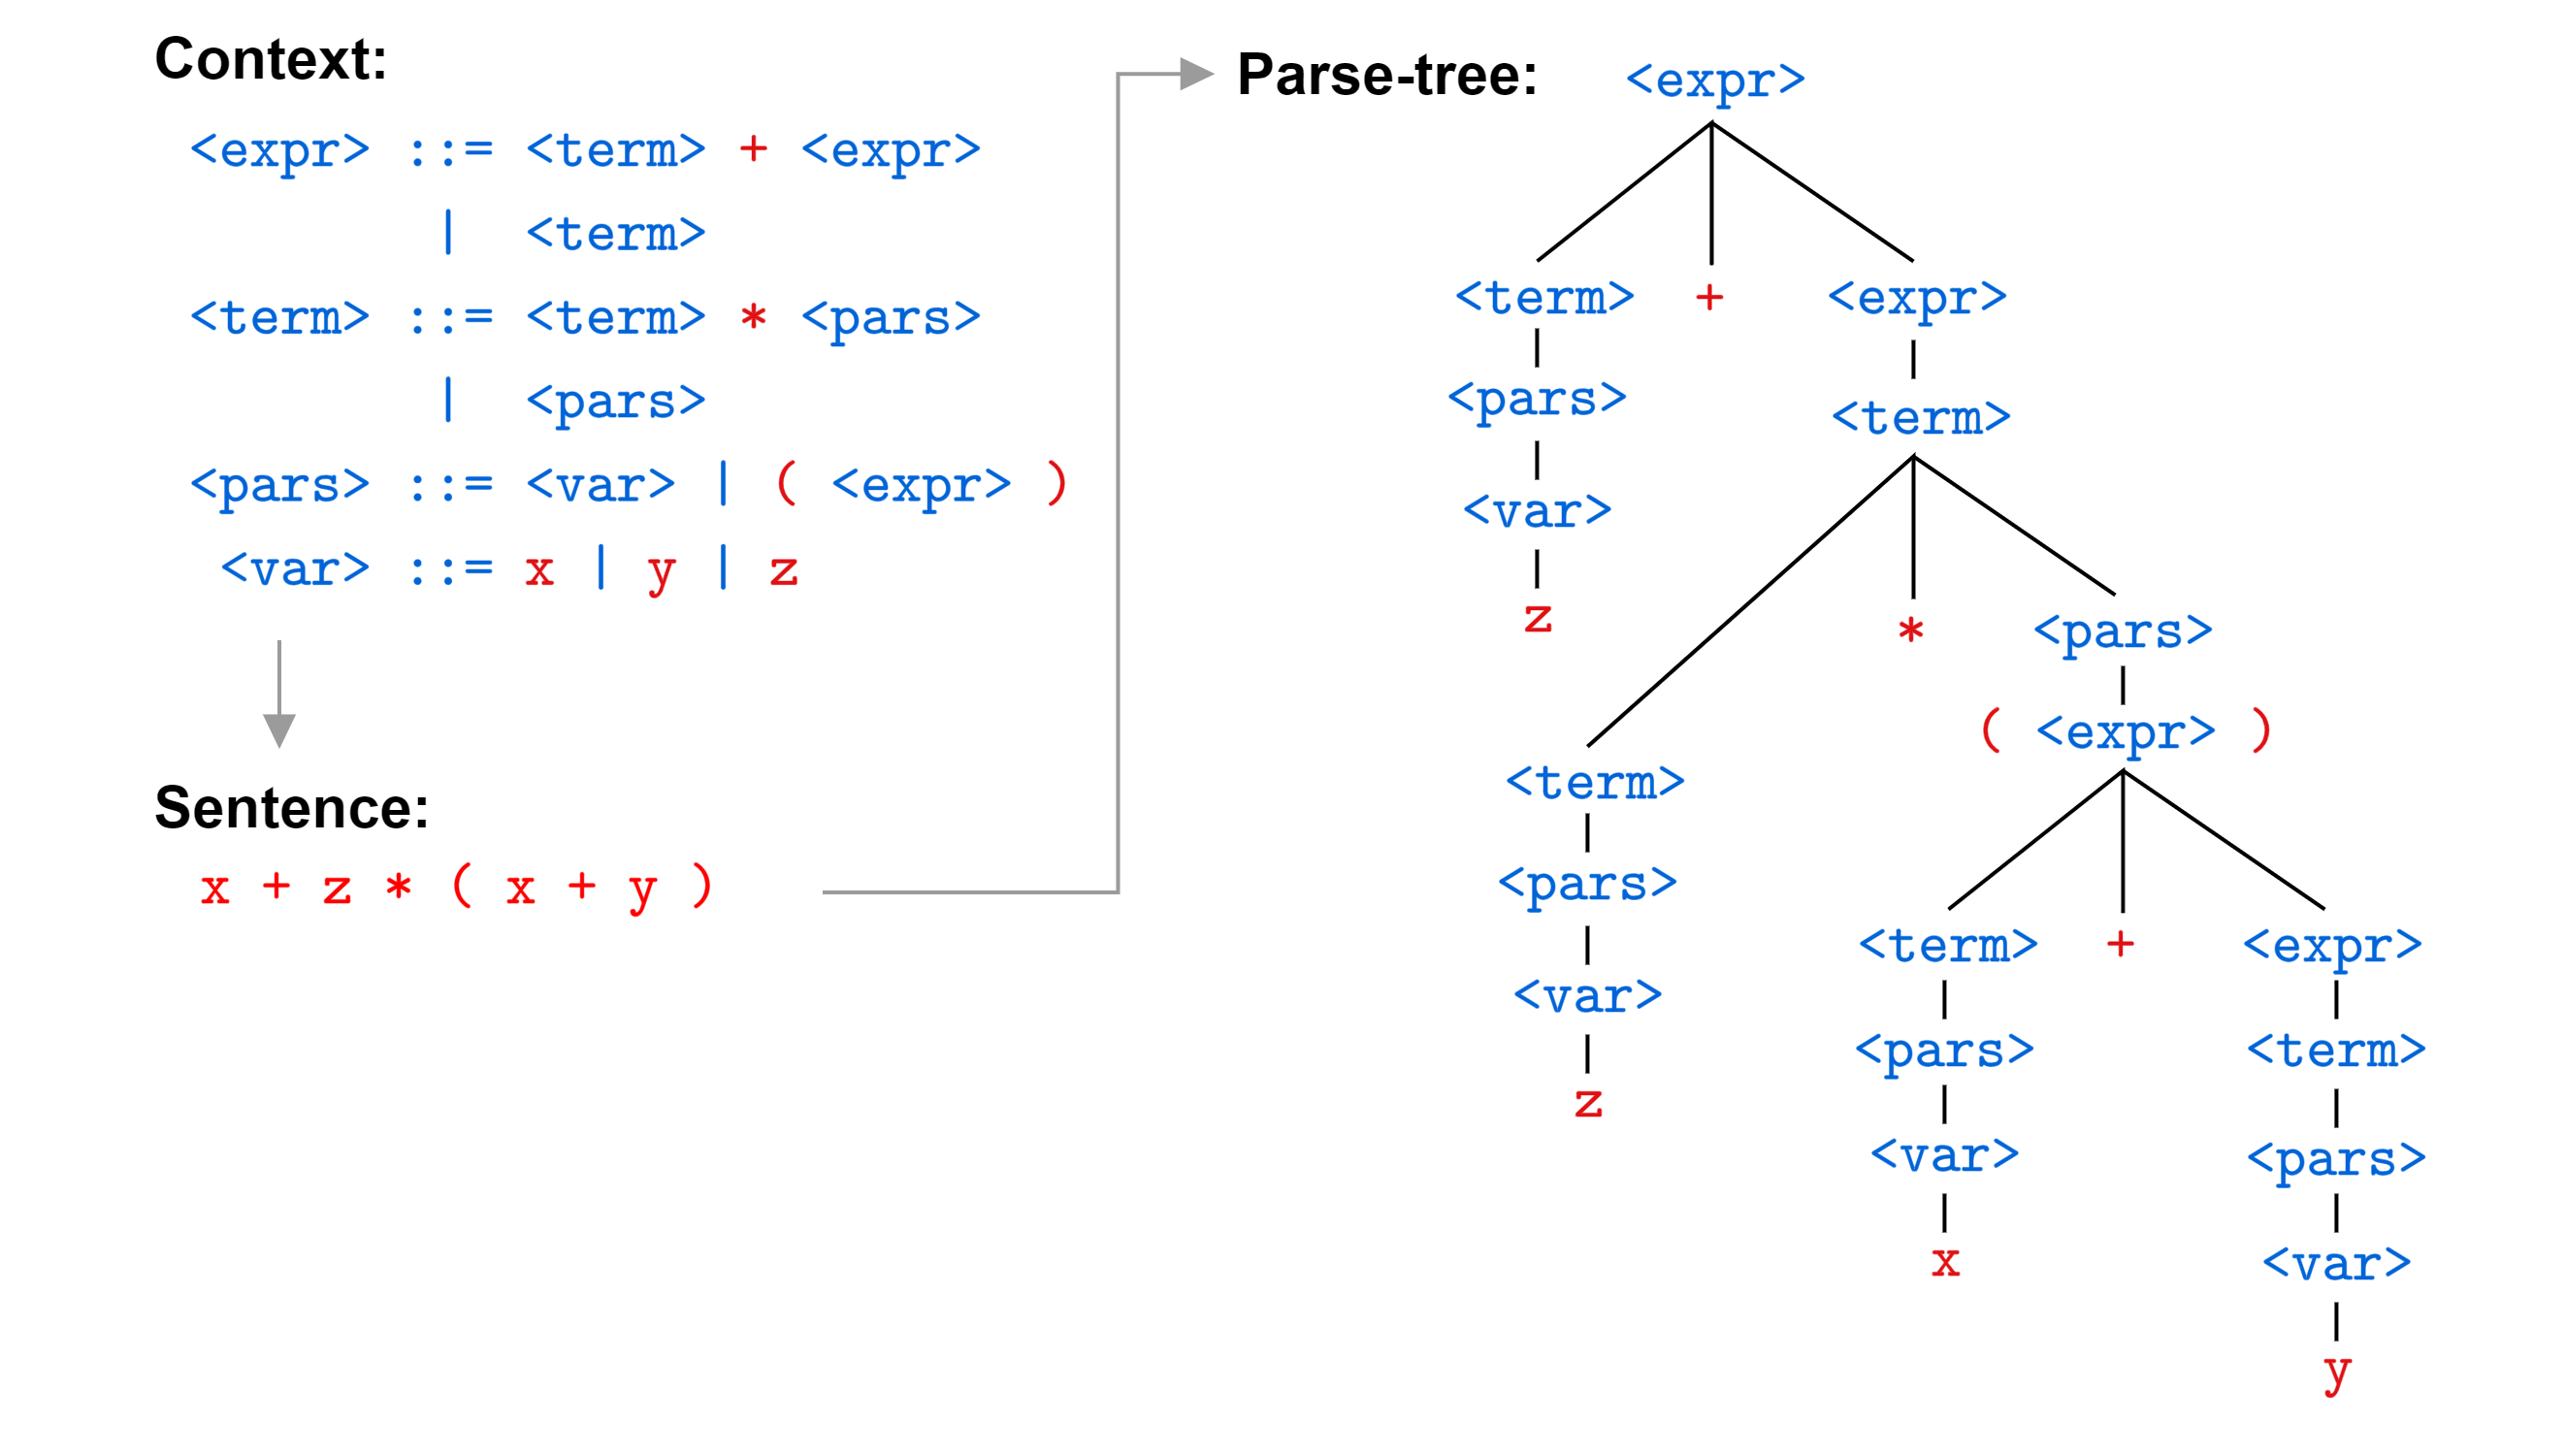
\includegraphics[width=1\textwidth]{Sections/Formal/amb6.png}
    \caption{An unambiguous grammar for \texttt{+, *} expressions, by breaking symmetry and precedence.}
    \label{fig:amb6}
\end{figure}

\begin{Tip} \textbf{The ``Cult of Parentheses" in Lisp:} Lisp-style languages rely heavily on \textbf{prefix notation}, where operators and function names appear \textbf{before} their arguments. This leads to deeply nested \textbf{parentheses}, often making Lisp code look overwhelming to newcomers.\\
    
    \noindent
    For example, the Fibonacci function in Lisp is written as:
    
    \begin{lstlisting}[numbers=none]
    (defun fib (n)
      "Return the nth Fibonacci number."
      (if (< n 2)
          n
          (+ (fib (- n 1))
             (fib (- n 2)))))
    \end{lstlisting}
    
    \noindent
    Since \textbf{everything} in Lisp is an expression and follows a \textbf{uniform syntax}, parentheses are required for every function call, condition, and operation. This often leads to \textbf{excessive nesting}.
    
    \end{Tip}
    
    
\section{Formal: Parsing, Lexing, Semantics, \& Grammar Types}
\subsection{Parsing Generators \& Grammar Types}


Lexical analysis and parsing are closely linked to 
compiler design. Though instead of writing such parsers by 
hand, we will use \textbf{parser generators}:

\begin{Def}[Parser Generators]

    \label{def:parser-generator}
    Parser generators are programs that take a representation of formal grammar as input and produces a parser as output.
\end{Def}

\noindent
We'll use \textbf{Menhir} for OCaml. There are other options but this suffices for our needs.
\begin{Def}[Menhir]

    Menhir is an LR(1) parser generator for OCaml. LR(1) stands for:
    \begin{itemize}
        \item \textbf{L}: Left-to-right scanning of the input.
        \item \textbf{R}: Rightmost derivation in reverse. Meaning, it builds the parse tree from the leaves up to the root.
        \item \textbf{(1)}: One symbol of lookahead. This means that the parser can look at one token ahead in the input stream to make parsing decisions.
    \end{itemize}
    \noindent
    Users input small OCaml snippets to define the production rules of the grammar.
\end{Def}

\newpage 

\noindent
A quick aside on Domain Specific Languages (DSLs):

\begin{Def}[Domain Specific Language (DSL)]

    A domain-specific language (DSL) is a programming language or specification language dedicated to a particular problem domain.
    An example of a DSL is SQL, as its only purpose is to query databases. This is in contrast to general-purpose languages like Python, which can be used for a wide range of applications.

    DSL's require custom parsers to be written. This can be done by hand, or using parser generators.
\end{Def}

\noindent
Now we discuss \textbf{Extended BNF (EBNF)}, which allows us to be more expressive in our grammars with less noise.

\begin{Def}[Extended BNF (EBNF)]

\label{def:ebnf}
Extended Backus-Naur Form (EBNF) is a notation for specifying formal grammars, building upon BNF (Backus-Naur Form) by introducing syntactic extensions for greater clarity and brevity.
EBNF includes the following additional constructs:

\begin{itemize}
    
    \item \texttt{|} — alternation: denotes choice between patterns.
    \begin{itemize}
        \item \textbf{E.g.,}  \snippet{<letter> ::= A | B | C}, means that <letter> can be A, B, or C.
    \end{itemize}
    \item \texttt{\{\ldots \}} — repetition: the enclosed pattern may repeat \underline{\textbf{zero} or more times}.
    \begin{itemize}
        \item \textbf{E.g.,}  \snippet{<digits> ::= \{0 | 1 | 2 | 3 | 4 | 5 | 6 | 7 | 8 | 9\}}, match:
        \begin{itemize}
            \item[>] \texttt{"0"}, \texttt{"320"}, \texttt{"11235813"}
        \end{itemize}
    \end{itemize}
    \item \texttt{[\ldots ]} — optionality: the enclosed pattern may appear zero or one time.
    \begin{itemize}
        \item \textbf{E.g.,} \snippet{<number> ::= ["-"] <digits>}, match:
        \begin{itemize}
            \item[>] \texttt{"1"}, \texttt{"-320"}
        \end{itemize}
    \end{itemize}
    \item \texttt{(\ldots )} — grouping: used to group sequences or alternatives.
    \begin{itemize}
        \item \textbf{E.g.,} \snippet{<sum> ::= <number> {("+" | "-") <number>}}, matches:
        \item [>] \texttt{"1 + 2 - 3"}, \texttt{"-1 + 2"}, \texttt{"5"}
        \end{itemize}
    \item \texttt{"\ldots"} — terminal strings may be written in quotes. This clears ambiguity between terminal and non-terminal symbols.
    \begin{itemize}
        \item \textbf{E.g.,} in \snippet{<digit> ::= A | B | C}, it's clear that A, B, and C refer to non-terminal symbols. However, in the expression \snippet{<expr> ::= <expr> | "(" <expr> ")"}, the parenthesis are \textbf{crucial} in indicating that it is not grouping notation.
    \end{itemize}
\end{itemize}
\end{Def}

\newpage

Let's elaborate more on \snippet{<digits>} from above:
\begin{Example}[Dealing with Optionality]

    In our previous grammar from Definition (\ref{def:ebnf}), we had:
    \begin{lstlisting}[numbers=none]
        <digit> ::= {0 | 1 | 2 | 3 | 4 | 5 | 6 | 7 | 8 | 9}
    \end{lstlisting}
    which matched:
    \begin{itemize}
        \item[>] \texttt{"0"}, \texttt{"320"}, \texttt{"11235813"}
    \end{itemize}

    \noindent
    But also unintentionally matched:
    \begin{itemize}
        \item[>] \texttt{""} \hfill \textit{(empty string)}
        \item[>] \texttt{"000"}, \texttt{"0123"} \hfill \textit{(leading zeros)}
    \end{itemize}
    
    \noindent
    Let's first fix the empty string case:
    \begin{lstlisting}[numbers=none]
        <digit> ::= 0 | 1 | 2 | 3 | 4 | 5 | 6 | 7 | 8 | 9
        <digits> ::= <digit> {<digit>}
    \end{lstlisting}

    \noindent
    To restrict leading zeros (e.g., for natural numbers), we refine further:
    \begin{lstlisting}[numbers=none]
        <nonzero> ::= 1 | 2 | 3 | 4 | 5 | 6 | 7 | 8 | 9
        <digits> ::= "0" | <nonzero> {<digit>}
    \end{lstlisting}

    \noindent
    Adding quotes around \snippet{0} is a stylistic choice and does not change the meaning of the grammar. We could have written:
    \begin{lstlisting}[numbers=none]
        <nonzero> ::= "1" | "2" | "3" | "4" | "5" | "6" | "7" | "8" | "9"
        <digits> ::= "0" | <nonzero> {<digit>}
    \end{lstlisting}
    \noindent
    Or without quotes, it doesn't matter as long as there is no ambiguity.
\end{Example}

\noindent
To be more precise with our language we briefly discuss \textbf{Automata Theory} and types of grammars:

\begin{Def}[Automata Theory]

    In mathematics, an automaton (Plural form: automata) is an abstract machine that follow a sequence of states (similar to a 
    flowchart). A finite number of states describe a \textbf{finite automaton (FA)} or \textbf{finite-state machine (FSM)}.
    \end{Def}

\begin{Tip}
    Automata comes from the Greek word $\alpha\upsilon\tau\acute{o}\mu\alpha\tau o\varsigma$ (autómatos), which means ``self-acting, self-willed, self-moving"
\end{Tip}

\newpage 


\noindent
Consider the following automaton described by a state machine diagram:

\begin{figure}[h]
    \centering
    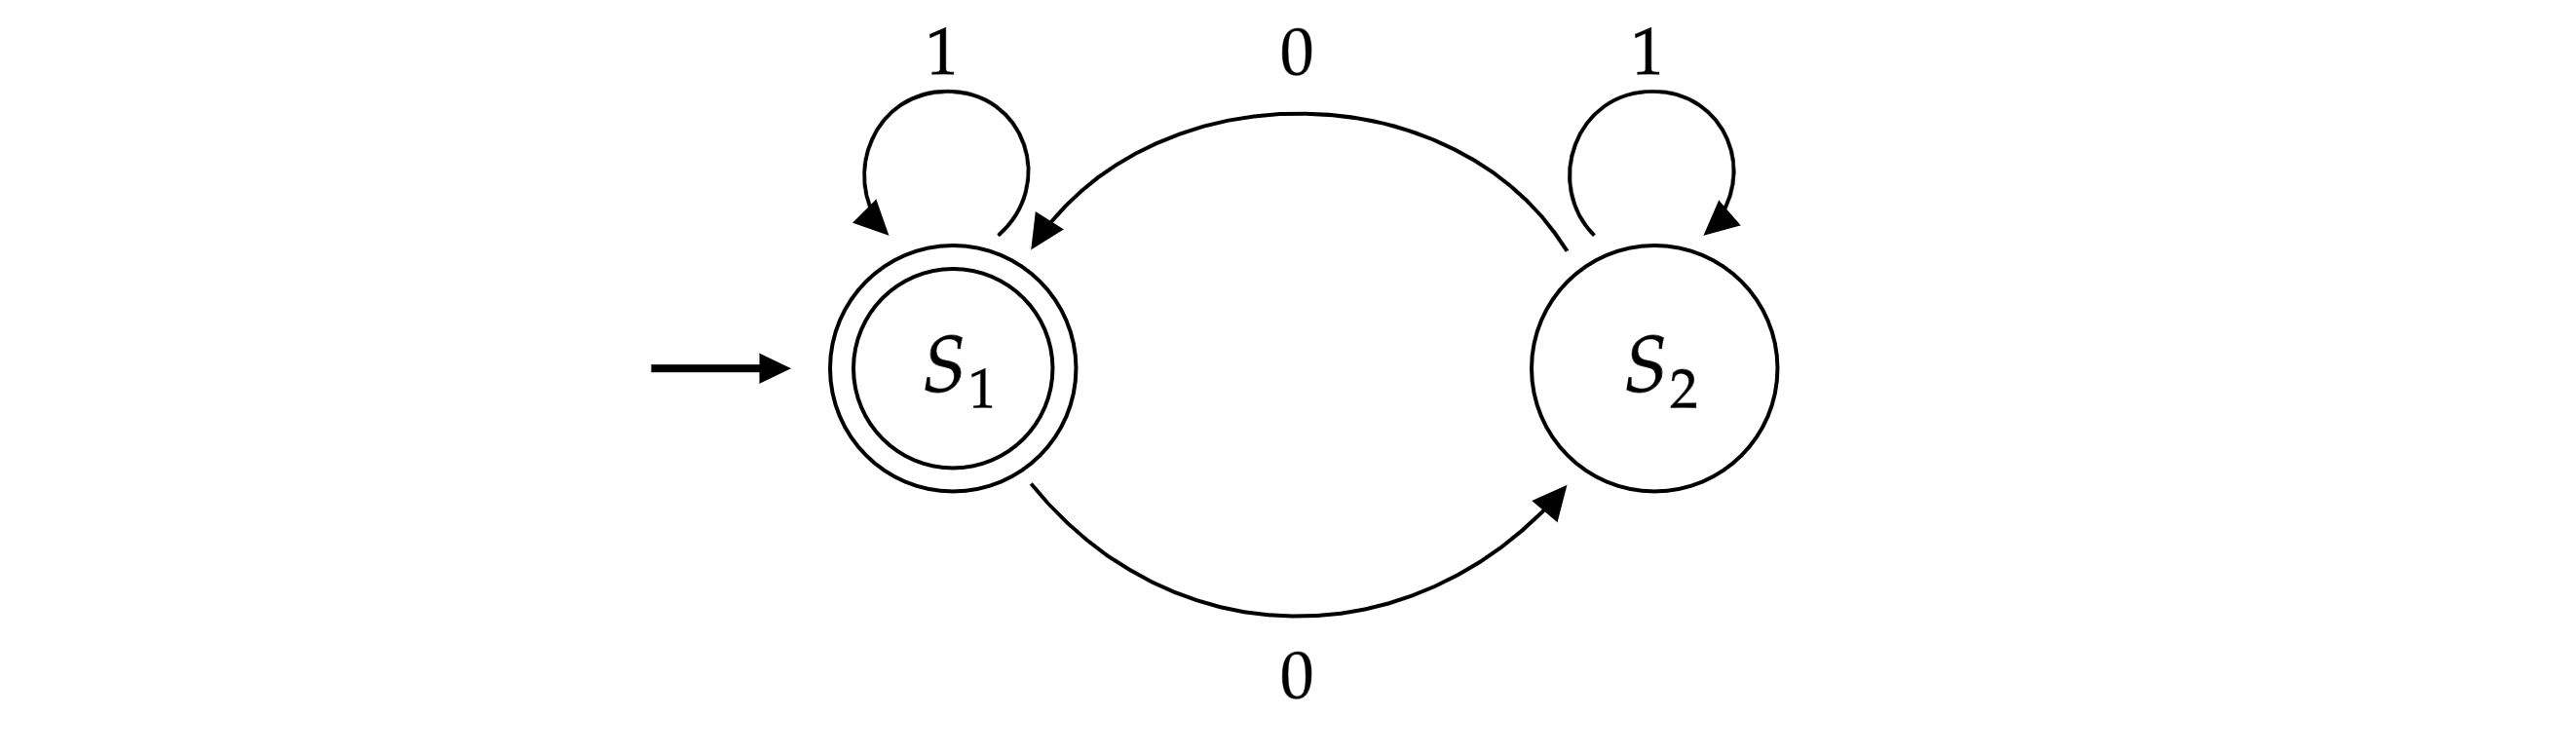
\includegraphics[width=\textwidth]{Sections/Parse/state.png}
    \caption{An automaton represented as a state-machine diagram. This state-machine generates binary strings with an even number of 0's.
    There are two states, $S_1$ and $S_2$. The automaton starts in state $S_1$ as shown by the arrow coming from blank space. The double
    circle indicates the \textbf{accepting state}, at which the automaton may terminate.}
    \label{fig:fa}
\end{figure}

\begin{Def}[Grammar Types]

    In formal language theory, grammars are classified into a hierarchy based on their generative power. This classification, known as the \textbf{Chomsky hierarchy}, comprises four primary types that utilize BNF:

    \begin{itemize}
        \item \textbf{Type 3: Regular Grammars} \\
        Generate \textbf{regular languages}, which can be recognized by finite automata. These grammars can describe simple flat patterns, but cannot handle nested or recursive structures.

        \item \textbf{Type 2: Context-Free Grammars (CFGs)} \\
        Generate \textbf{context-free languages} and are recognized by pushdown automata. A \textbf{pushdown automaton} is a finite automaton extended with a stack—a Last-In, First-Out (LIFO) memory structure. This allows it to handle nested and recursive structures, such as balanced parentheses.

        \item \textbf{Type 1: Context-Sensitive Grammars} \\
        Generate \textbf{context-sensitive languages} and are recognized by linear bounded automata. A \textbf{linear bounded automaton} is a Turing machine where the tape is limited to a length proportional to the input size. This constraint gives it more power than pushdown automata but less than unrestricted Turing machines.

        \item \textbf{Type 0: Unrestricted Grammars} \\
        Generate \textbf{recursively enumerable languages} and are recognized by Turing machines. These grammars have no restrictions on production rules and can describe any computable language, though some of these languages are undecidable.
    \end{itemize}
\end{Def}

\newpage 

\noindent
We can visualize the Chomsky hierarchy as follows:

\begin{figure}[h]
    \centering
    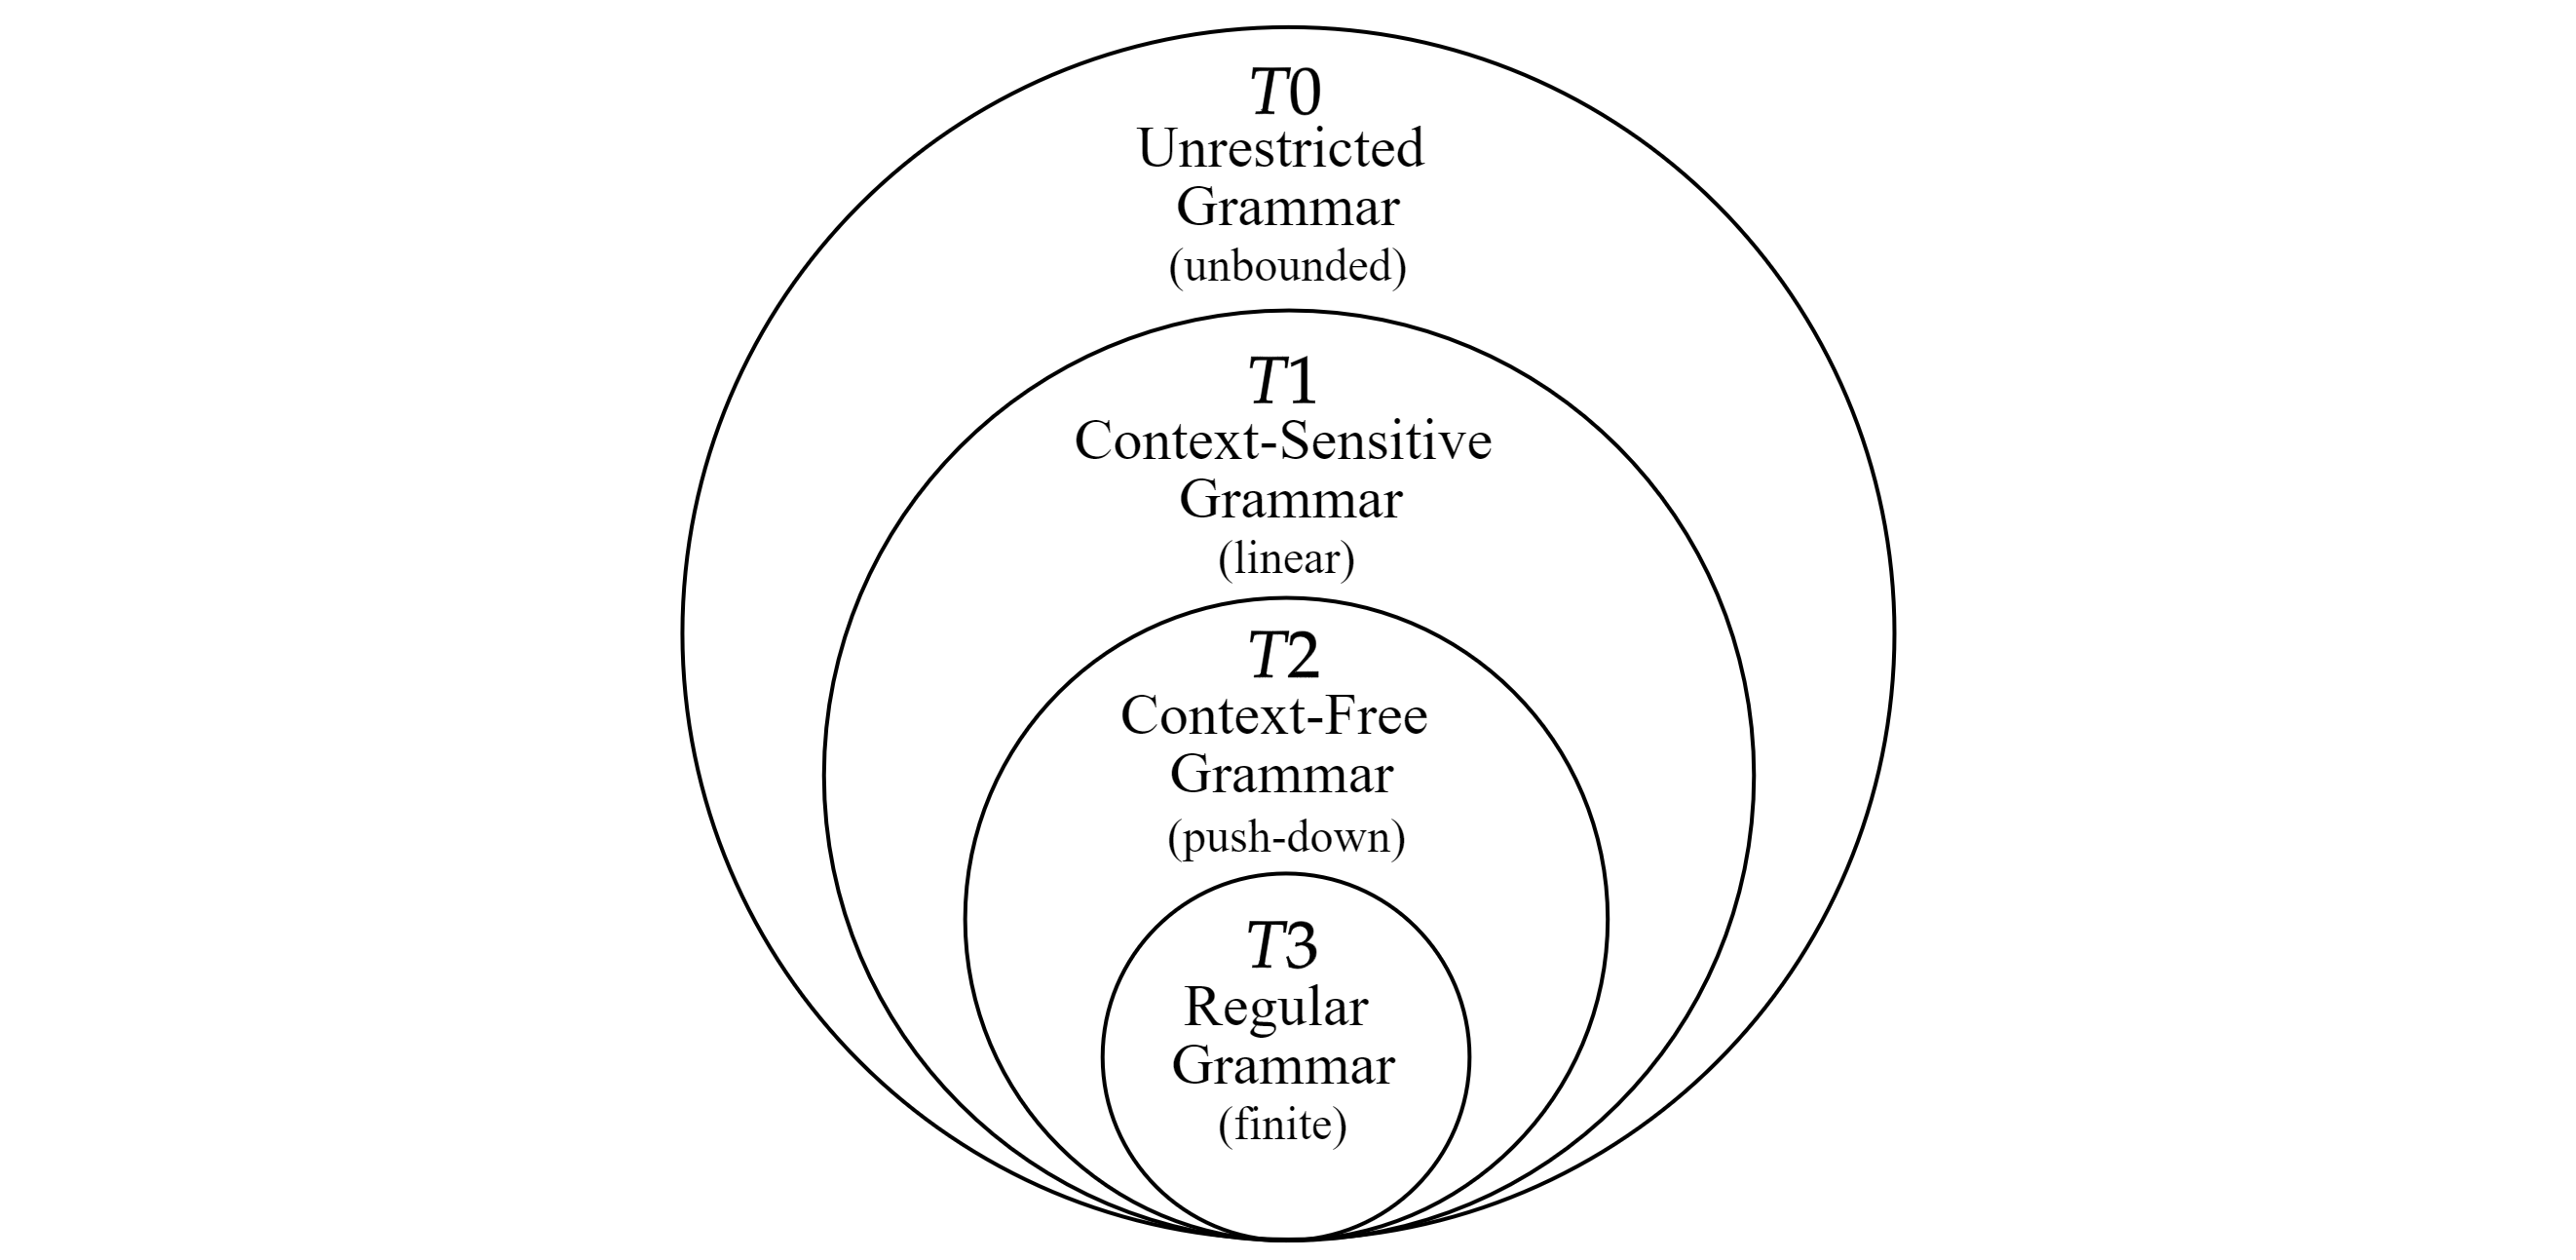
\includegraphics[width=\textwidth]{Sections/Parse/chom.png}
    \caption{
        The Chomsky hierarchy: 
        $T_3$ finite automata (regular expressions), 
        $T_2$ pushdown automata (context-free grammars),
        $T_1$ linear bounded automata (context-sensitive grammars),
        and $T_0$ Turing machines (unrestricted grammars).
    } 
    \label{fig:chomsky}
\end{figure}

\begin{Def}[Regular Expressions (Regex)]

    \label{def:regex}
    Regular expressions (Regex) provide a compact way to describe patterns in regular grammars:
    
    \begin{itemize}
        \item \texttt{a} — a single \textbf{terminal} symbol is itself a regex.
       
    
        \item \texttt{[t1 t2 \ldots tk]} — character class: matches any one of the listed characters.
        
    
        \item \texttt{(e1 | e2 | \ldots | ek)} — alternation: matches any one of the enclosed expressions.
       
    
        \item \texttt{exp*} — repetition: matches \underline{\textbf{zero or more occurrences}} of \texttt{exp}.
      
    
        \item \texttt{exp+} — repetition: matches \underline{\textbf{one or more occurrences}} of \texttt{exp}.
        
    
        \item \texttt{exp?} — optional: matches \underline{\textbf{zero or one occurrence}} of \texttt{exp}.
        
    \end{itemize}
    
    \noindent
    \textbf{E.g.,} the regex \texttt{(a|b)*c} matches any string of a's and b's followed by a c, such as:
    \begin{itemize}
        \item[>] \texttt{"abc"}, \texttt{"aabbbbc"}, \texttt{"c"}
    \end{itemize}
   
    \noindent
    This is just a small subset of the Regex syntax. To learn more, consider the following resource:
    \url{https://regexlearn.com/}
    \end{Def}
\newpage 
\subsection{Menhir: Simple Lexing \& Parsing }
\noindent
To formally retouch on the definitions of lexing:

\begin{Def}[Lexical Analysis]

    \label{def:lexical-analysis}
    Lexical analysis concerns itself with the \textbf{tokenization} of a program. In particular, converting a stream 
    of characters into a stream of tokens (whitespace and comments are ignored).

    Lexing (to lex) works by scanning the input for the next longest valid token. Then 
    it returns that token and the remaining input to lex.\\

    \noindent
    \textbf{E.g.,} \snippet{" let@\#\_)(\$\#@\_J\_@O\#GKJ"} gives us \snippet{(LET, "@\#\_)(\$\#@\_J\_@O\#GKJ")}, where 
    \snippet{LET} is the token and \snippet{"@\#\_)(\$\#@\_J\_@O\#GKJ"} is the remaining input, which is most likely to result in an error 
    (unless the lexer is designed to handle such cases).
\end{Def}

\noindent
We will now create a lexer and parser for a simple toy-language that only has 
addition, subtraction, multiplication, and division.
Menhir should already be installed from the onboarding Section (\ref{subsec:opam_packages}).



\begin{Example}[Simple Lexer \& Parser (Part 1)]

    \label{ex:lexer-parser}
    Let's create a simple lexer and parser for a toy language that only has addition, subtraction, multiplication, and division.
    We will use Menhir to generate the parser.\\

    \noindent
    Let's create the project: 
    \begin{lstlisting}[numbers=none]
        dune init proj small_arith
        cd small_arith
    \end{lstlisting}

    \noindent
    This should create: \\

    \noindent
    \rule{\textwidth}{0.4pt} 
    \dirtree{%
    .1 small\_arith/.
    .2 \_build/.
    .3 log.
    .2 bin/.
    .3 dune.
    .3 main.ml.
    .2 dune-project.
    .2 lib/.
    .3 dune.
    .2 small\_arith.opam.
    .2 test/.
    .3 dune.
    .3 test\_small\_arith.ml.
    }
    \noindent
    \rule{\textwidth}{0.4pt} \\
\end{Example}


\newpage 

\begin{Example}[Simple Lexer \& Parser (Part 2)]

    \noindent
    Create these new files, \snippet{lib/ast.ml}, \snippet{lib/lexer.mll}, and \snippet{lib/parser.mly}:
    \begin{lstlisting}
        touch lib/dune lib/ast.ml lib/lexer.mll lib/parser.mly
    \end{lstlisting}

\begin{itemize}
    \item \snippet{ast.ml} — A regular OCaml source file (\texttt{.ml}) where we define the core data structures via ADTs, which will generate the \textbf{abstract syntax tree (AST)} for our language.

    \item \snippet{lexer.mll} — The (\texttt{.mll}) extension to signal it will be processed by \textbf{OCamllex}, a lexer generator. Here, we write rules using regular-expression-like syntax to convert raw strings into \textbf{tokens} like \texttt{NUM}, \texttt{ADD}, and \texttt{LPAREN}.

    \item \snippet{parser.mly} — The (\texttt{.mly}) extension is handled by \textbf{Menhir}. It defines the \textbf{grammar} of our language. The result of parsing is an AST defined in \snippet{ast.ml}.
\end{itemize}

\noindent
\textbf{Together:} 
\texttt{Input String} $\rightarrow$ \texttt{Lexer (mll)} $\rightarrow$ \texttt{Tokens} $\rightarrow$ \texttt{Parser (mly)} $\rightarrow$ \texttt{AST (ml)}

\noindent
\rule{\textwidth}{0.4pt}\\

\noindent
Lets begin by defining the AST in \snippet{ast.ml}:
\begin{lstlisting}[numbers=none]
    (* ast.ml *)
    type bop = Add | Sub | Mul | Div 
    
    type expr =
      | Var of string
      | Num of int
      | Let of string * expr * expr
      | Bop of bop * expr * expr
    
    type prog = expr
    \end{lstlisting}

\noindent
    The above code defines the abstract syntax tree (AST) for our toy language. It includes:
    \begin{itemize}
        \item \texttt{bop} — a type for binary operators (addition, subtraction, multiplication, division).
        \item \texttt{expr} — a type for expressions, which can be a variable, number, let-binding, or binary operation.
        \item \texttt{prog} — a type for the program, which is just an expression.
    \end{itemize}

    \noindent
    This should be familiar from the BNF grammar we've discussing.
\end{Example}

\newpage 


\begin{Example}[Simple Lexer \& Parser (Part 4)]

    Now let's define our lexer in \snippet{lib/lexer.mll}:
    
    \begin{lstlisting}[numbers=none]
    (* lexer.mll *)
    {
        open Parser
    }

    (* Regex for tokens *)
    let whitespace = [' ' '\t' '\n' '\r']+
    let var = ['a'-'z' '_'] ['a'-'z' 'A'-'Z' '0'-'9' '_' '\'']*
    let num = ['0'-'9']+

    rule read = parse
        | whitespace { read lexbuf }
        | "let"      { LET }
        | "in"       { IN }
        | "="        { EQ }
        | "+"        { ADD }
        | "-"        { SUB }
        | "*"        { MUL }
        | "/"        { DIV }
        | "("        { LPAREN }
        | ")"        { RPAREN }
        | num        { NUM (int_of_string (Lexing.lexeme lexbuf)) }
        | var        { VAR (Lexing.lexeme lexbuf) }
        | eof        { EOF }
    \end{lstlisting}
    
    \begin{itemize}
        \item \snippet{lexbuf}: short for \textbf{``lexing buffer,''} is an object created by the OCaml stdlib. It stores the input string and tracks the position of the lexer as it reads through.
        
        \item \snippet{read lexbuf}: A recursive call to the lexer function. It's used to \textbf{skip over whitespace}. When the lexer sees a space or newline, it just calls itself again to scan the next part of the input.
    
        \item \snippet{Lexing.lexeme lexbuf}: This function returns the \textbf{exact substring} that was matched by our Regex.
         For example, if the input is \texttt{"42 + 1"} and we match \snippet{num}, then\\
        \snippet{Lexing.lexeme lexbuf} returns \texttt{"42"} as a string. We then convert it to an integer.

        \item \snippet{rule read = parse}: This defines the main lexer function. The \snippet{read} is the entry point of the lexer. The \snippet{parse} keyword indicates parsing rules for the input to match against.
    \end{itemize}
    
    
\end{Example}
        
\newpage 

\begin{Example}[Simple Lexer \& Parser (Part 5)]

    Finally the parser in \snippet{lib/parser.mly} utilizing our \snippet{ast.ml} (Moreover on the next page.):
    
    \begin{lstlisting}[numbers=none]
    %{
      open Ast
    %}
    
    %token LET EQ IN
    %token ADD SUB MUL DIV
    %token LPAREN RPAREN
    %token <int> NUM
    %token <string> VAR
    %token EOF
    
    %left ADD SUB
    %left MUL DIV
    
    %start <Ast.prog> prog
    %%
    
    prog:
      | e = expr; EOF { e }
    
    expr:
      | LET; x = var; EQ; e1 = expr; IN; e2 = expr
        { Let (x, e1, e2) }
      | e = expr1 { e }
    
    %inline bop:
      | ADD { Add }
      | SUB { Sub }
      | MUL { Mul }
      | DIV { Div }
    
    expr1:
      | e1 = expr1; op = bop; e2 = expr1
        { Bop (op, e1, e2) }
      | n = num { Num n }
      | v = var { Var v }
      | LPAREN; e = expr; RPAREN { e }
    
    num:
      | n = NUM { n }
    
    var:
      | x = VAR { x }
    \end{lstlisting}

    \noindent
    
    \end{Example}
    

    \begin{Example}[Simple Lexer \& Parser (Part 5a)]

        The \snippet{parser.mly} file looks quite different from regular OCaml code because it follows the syntax of Menhir (an LR(1) parser generator). Let's walk through its structure:
        
        \begin{itemize}
            \item \snippet{\%\{ ... \%\}} — Opens a block of OCaml code. We use it to import our AST module.
        
            \item \snippet{\%token} — Declares the tokens the parser will receive from the lexer. If tokens carry data integer or string, we write it as:
            \begin{lstlisting}[numbers=none]
        %token <int> NUM
        %token <string> VAR
            \end{lstlisting}
        
            \item \snippet{\%left} — Defines left-associativity, and precedence is by order of declaration:
            \begin{lstlisting}[numbers=none]
        %left ADD SUB
        %left MUL DIV
            \end{lstlisting}
            means that \snippet{MUL} and \snippet{DIV} bind more tightly than \snippet{ADD} and \snippet{SUB}. All are left-associative. This prevents ambiguity in expressions like \texttt{3 + 4 * 2}.
        
            \item \snippet{\%start <Ast.prog> prog} — The entry point of the parser is the rule \snippet{prog}. The return type is \snippet{Ast.prog} from our AST module.
           
        
            \item \snippet{<name>:} — Each rule has the form:
            \begin{lstlisting}[numbers=none]
        name:
          | pattern1 { action1 }
          | pattern2 { action2 }
            \end{lstlisting}
            Think of it as EBNF, but instead we use OCaml pattern matching syntax.
        
            \item \snippet{\%inline <name>:} — A helper rule that lets us \textbf{macro} grammar patterns into a single variable without generating a new nonterminal or type (cannot be recursive):
            \begin{lstlisting}[numbers=none]
        %inline bop:
          | ADD { Add }
          | SUB { Sub }
          | ...
            \end{lstlisting}
        
        \end{itemize}
        \end{Example}

        \newpage 

\begin{Example}[Simple Lexer \& Parser (Part 5b)]

    Let's look closely at the following grammar rule:
    
    \begin{lstlisting}[numbers=none]
    expr:
        | LET; x = var; EQ; e1 = expr; IN; e2 = expr
        { Let (x, e1, e2) }
    \end{lstlisting}
    
    \begin{itemize}
        \item Each item before the `\texttt{\{}' is a \textbf{token} (e.g., \snippet{LET}, \snippet{EQ}, \snippet{IN}) or a \textbf{nonterminal rule} (e.g., \snippet{var}, \snippet{expr}).
        \item When a nonterminal is matched, we can bind its result using \snippet{name = rule}. For example, \snippet{x = var} means: “run the \snippet{var} rule and bind its result to \snippet{x}.”
        \item The block in \texttt{\{ \}} is an OCaml expression that builds an AST node using the bound variables.
        Notice, \snippet{Let (x, e1, e2)} our ADT constructor from \snippet{ast.ml}.
    \end{itemize}
    
    \noindent
    \rule{\textwidth}{0.4pt}\\

    \noindent
    When we parse a string like:
    
    \begin{lstlisting}[numbers=none]
    let x = 3 + 4 in x * 2
    \end{lstlisting}
    
    \noindent
    The lexer produces a stream of tokens:
    
    \begin{lstlisting}[numbers=none]
 [LET; VAR("x"); EQ; NUM(3); ADD; NUM(4); IN; VAR("x"); MUL; NUM(2); EOF]
    \end{lstlisting}
    
    \noindent
    Then, the parser:
    \begin{itemize}
        \item Sees \snippet{LET}, then \snippet{VAR("x")} → runs the \snippet{var} rule, binds to \snippet{x}.
        \item Sees \snippet{EQ}, then parses the expression \snippet{3 + 4} using the \snippet{expr} rule, binds to \snippet{e1}.
        \item Sees \snippet{IN}, then parses the expression \snippet{x * 2}, binds to \snippet{e2}.
    \end{itemize}
    
    \noindent
    Finally, it constructs:
    
    \begin{lstlisting}[numbers=none]
    Let (x, e1, e2)
    \end{lstlisting}
    
    \noindent
    This is now a fully constructed OCaml value using the constructors we defined in \snippet{ast.ml}.
    
    \end{Example}
            
    \newpage 

\begin{Example}[Setting Up Dune and Testing in \texttt{utop}]

    Now that we've written our AST, lexer, and parser, we need to set up Dune so we can compile everything and test it in \texttt{utop}.\\
    
    \noindent
    First, open your \snippet{dune-project} file and add the following line at the bottom to enable Menhir:
    
    \begin{lstlisting}[numbers=none]
    (using menhir 3.0)
    \end{lstlisting}
    
    \noindent
    Your complete \snippet{dune-project} should now look like:
    
    \begin{lstlisting}[numbers=none]
    (lang dune 3.0)
    (name small_arith)
    (using menhir 3.0)
    \end{lstlisting}
    
    \noindent
    Next, open \snippet{lib/dune}:
    
    \begin{lstlisting}[numbers=none]
    (library
        (name small_arith))
    
    (ocamllex lexer)
    (menhir (modules parser))
    \end{lstlisting}
    
    \noindent
    Create a \snippet{lib/demo.ml} file to test the lexer and parser:
    \begin{lstlisting}[numbers=none]
    let parse s =
        try Some (Parser.prog Lexer.read (Lexing.from_string s))
        with _ -> None
    \end{lstlisting}
    
    \noindent
    From the root of your project, run:
    
    \begin{lstlisting}[numbers=none]
    dune build
    dune utop lib
    \end{lstlisting}
    
    \noindent
    In \texttt{utop}, you can test the parser like this:
    
    \begin{lstlisting}[numbers=none]
    # Demo.parse "let x = 3 + 4 in x * 2";;
    - : Demo__Ast.prog option =
    Some
    (Demo__.Ast.Let ("x",
    Demo__.Ast.Bop (Demo__.Ast.Add, Demo__.Ast.Num 3, Demo__.Ast.Num 4),
    Demo__.Ast.Bop (Demo__.Ast.Mul, Demo__.Ast.Var "x", Demo__.Ast.Num 2)))
    \end{lstlisting}
    \end{Example}
        
        
        
\newpage
\section{Semantic Evaluation}
\subsection{Small-step Semantics}

\noindent
In our previous derivations, we've been doing \textbf{Big-step semantics}:

\begin{Def}[Big-Step Semantics]

    Big-step semantics describes how a complete expression evaluates directly to a final value, without detailing each intermediate step. It relates an expression to its result in a single derivation.
    
    \medskip
    \noindent\textbf{Notation:} We write $e \Downarrow v$ to mean that the expression $e$ evaluates to the value $v$.\\
    \noindent\textbf{Example:}
    \[
    (\text{sub}\ 10\ (\text{add}\ (\text{add}\ 1\ 2)\ (\text{add}\ 2\ 3))) \Downarrow 2
    \]
    \end{Def}

\noindent
Here, we now introduce \textbf{Small-step semantics}:

\begin{Def}[Small-Step Semantics]

    Small-step semantics describes how an expression is reduced one step at a time. Each step transforms the current expression into a simpler one until no further reductions are possible.
    \noindent\textbf{Notation:} We write $e \rightarrow e'$ to mean that $e$ reduces to $e'$ in a single step.
    The notation:
    \begin{center}
    \LARGE
    $\underbracket{(S,p)}_{\text{configuration}} \longrightarrow \underbracket{(S',p')}_{\text{transformation.}}$
    \normalsize
    \end{center}
    \noindent
    Where $S$ is the state of the program and $p$ is the program. The rightarrow shows the \textbf{transformation} or \textbf{reduction} of the program. Since
    for our purposes OCaml \textit{doesn't} have state, so we'd typically write:
    \begin{center}
    \LARGE
    $(\varnothing, p) \longrightarrow (\varnothing,p')$
    \normalsize
    \end{center}
    \noindent
    Hence, moving forward we \underline{shorthand this to $p \rightarrow p'$} for brevity. We may describe the semantics for 
    grammars in terms of small-step semantics using inference rules:
    \Large
    \[
    \begin{prooftree}
    \hypo{e_1 \rightarrow e_1'}
    \Infer1[(\text{reduction})]{e_1 + e_2 \longrightarrow e_1' + e_2}
    \end{prooftree}
    \]
    \normalsize
    \noindent
    Where $e$ is a well-formed expression that can be reduced to $e'$, hence our premise ``$e \rightarrow e'$''.

\end{Def}

\newpage

\noindent
We can use these small-step semantics to define evalutions in our grammar:

\begin{Example}[Defining Grammars in Small-Step Semantics]
    
    \label{ex:small-step-semantics}
    Say we have part of some toy-language grammar:
    \begin{lstlisting}[numbers=none]
    <expr> ::= ( <op> <expr> <expr> )
            | <int>
    <op>   ::= add | sub | eq
    <int>  ::= ...
    \end{lstlisting}

    \noindent
    Let's assume our language reads from left to right and define the semantics of \texttt{add}:
    \begin{itemize}
        \item \textbf{Both arguments are expressions:}
        \[
        \begin{prooftree}
        \hypo{\text{add}\ e_1 \rightarrow e_1'}
        \Infer1[\text{(add-left)}]{ (\text{add}\ e_1\ e_2) \rightarrow (\text{add}\ e_1'\ e_2) }
        \end{prooftree}
        \]
        \item \textbf{Left argument is an integer:}
        \[
        \begin{prooftree}
        \hypo{n \text{ is an integer literal}\qquad e_2 \rightarrow e_2'}
        \Infer1[\text{(add-right)}]{ (\text{add}\ n\ e_2) \rightarrow (\text{add}\ n\ e_2') }
        \end{prooftree}
        \]
        \item \textbf{Both arguments are integers:}
        \[
        \begin{prooftree}
        \hypo{n_1 \text{ and } n_2 \text{ are integer literals}}
        \Infer1[\text{(add-ok)}]{ (\text{add}\ n_1\ n_2) \rightarrow n_1 + n_2 }
        \end{prooftree}
        \]
    \end{itemize}

    \noindent
    The intuition is to think about our grammar, in this case \textbf{add}, and think, ``What are all the possible argument states of add?''
    If we have \texttt{(add <expr> <expr>)}, we have to reduce \texttt{<expr>} before we can evaluate it. In cases like 
    \texttt{(add 1 2)}, there is nothing left to reduce.\\

    \noindent
    We can almost think of these terminal-symbols as \textbf{base cases}.
    Additionally, since we read left to right, \texttt(add <expr> 2) is impossible, as we should have evaluated the left-hand side first.

\end{Example}
        
\begin{Tip}
    States can represent data structures like stacks, making them ideal for modeling stack-oriented languages. For example ($\epsilon$ is the empty program):
    \begin{align*}
    &(\varnothing,\ \texttt{push 2;\ push 3;\ add}) \\
    \rightarrow\quad &(2\ \texttt{::}\ \varnothing,\ \texttt{push 3;\ add}) \\
    \rightarrow\quad &(3\ \texttt{::}\ 2\ \texttt{::}\ \varnothing,\ \texttt{add}) \\
    \rightarrow\quad &(5\ \texttt{::}\ \varnothing,\ \epsilon)
    \end{align*}

\end{Tip}
    
\newpage
\begin{Def}[Multi-Step Semantics]

    Multi-step semantics captures the idea of reducing a configuration through \textbf{zero or more \underline{single-step reductions}}.
    We write $C \rightarrow^{\star} D$ to mean that configuration $C$ reduces to configuration $D$ in zero or more steps.
This relation is defined inductively with two rules:
    
\Large
    \begin{center}
    \begin{minipage}{0.45\textwidth}
        \centering

        \vspace{{.5em}}
        \begin{prooftree}
        \infer0[(reflexivity)]{C \rightarrow^{\star} C}
        \end{prooftree}
    \end{minipage}
    \hfill
    \begin{minipage}{0.45\textwidth}
        \begin{prooftree}
        \hypo{C \rightarrow C'}
        \hypo{C' \rightarrow^{\star} D}
        \infer2[(transitivity)]{C \rightarrow^{\star} D}
        \end{prooftree}
    \end{minipage}
    \end{center}
    
    \normalsize
    \noindent
    These rules formalize:
    \begin{itemize}
        \item Every configuration reduces to itself \hfill \textit{(reflexivity)}
        \item Multi-step reductions can be extended by single-step reductions \hfill \textit{(transitivity)}
        \item If there are multiple ways to reduce $C\rightarrow^\star D$, then the semantics are \textbf{ambiguous}.
    \end{itemize}
    \end{Def}
    
\begin{Example}[Multi-step Reduction]

    \noindent
    We show (add (add 3 4) 5)$\rightarrow^{\star} 14$ based off the semantics we defined in Example (\ref{ex:small-step-semantics}). We 
    will do multiple rounds of single-step reductions to yield a final value:
    \begin{enumerate}
    \item \hspace{6em}
    \begin{prooftree}
        
        \Infer0[(add-ok)]{\text{add 3 4} \rightarrow 7}
        \Infer1[(add-right)]{\text{add 5 (add 3 4)} \rightarrow \text{add 5 7}}
        \Infer1[(add-left)]{\text{(add (add 5 (add 3 4)) 2)} \rightarrow \text{(add (add 5 7) 2)}}
    \end{prooftree}

    \vspace{2em}    
    
    \item \hspace{8em}
    \begin{prooftree}
        \Infer0[(add-ok)]{\text{(add 5 7)} \rightarrow 12}
        \Infer1[(add-left)]{\text{(add (add 5 7) 2)} \rightarrow \text{(add 12 2)}}
    \end{prooftree}

    \vspace{2em}   

    \item \hspace{12em}
    \begin{prooftree}
        \Infer0[(add-ok)]{\text{(add 12 2)} \rightarrow 14}
    \end{prooftree}\\

    \end{enumerate}
    Thus, $\text{(add (add 3 4) 5)} \rightarrow^{\star} 14$. When deriving, we think like a compiler, and grab the next recursive call to reduce. Notice how our very first reduction matches with 
    (add-left). In particular, $e_1:=$ (add 5 (add 3 4)), and we see that's our starting value the next layer up.\\

    \noindent
    Moreover, the trailing 2 in (add (add 5 (add 3 4)) 2), is not evaluated until the very last step (3), as we read from left-to-right.
    Even though \textit{we can see it}, the computer does not.

\end{Example}

\newpage 

\noindent
Though there is a clear distinction between big-step and small-step semantics:

\begin{theo}[Small-Step vs. Big-Step Semantics]

    Multi-step semantics bridges small-step and big-step semantics:
    \Large
    \[
      e \rightarrow^\star v \quad \approx \quad e \Downarrow v
    \]
    \normalsize
    Where a well-formed expression \( e \) reduces to a value \( v \) via zero or more single-step reductions. This is approximately what big-step semantics aims to accomplish
    without underlying intermediate steps.\\
  
    \noindent
    Unlike big-step semantics, small-step semantics allows us to choose how we reduce our terms in every step, and \textbf{in which order}. This eliminates possible ambiguity in the grammar.
\end{theo}
  
\subsection{Lambda Calculus}

\noindent
We briefly touched on \textbf{Lambda Calculus} in a previous section when discussing the Anonymous Function Definition (\ref{def:anon-func}). Here
we go more in-depth:

\begin{Def}[Lambda Calculus Syntax]

    Lambda calculus is a formal system for representing computations using only single-argument functions, avoiding the need for multiple parameters or state. Lambda calculus has three basic constructs:
    \begin{itemize}
      \item \textbf{Variables:} \(x\), \(y\), \(z\), etc.
      \item \textbf{Abstraction:} \(\lambda x. e\) (a function that takes an argument \(x\) and returns expression \(e\)).
      \item \textbf{Application:} \(e_1\, e_2\) (applying function \(e_1\) to argument \(e_2\)).
    \end{itemize}
  
    \noindent
    In particular:
    \LARGE
    \[
        \lambda x. e \quad \equiv \quad \texttt{fun } x \texttt{ -> } e
    \]\\
    \normalsize
    \noindent
    Where we replace the `\texttt{fun}' with `$\lambda$', and `\texttt{->}' with `\texttt{.}'.
  \end{Def}
  
  \begin{Def}[The Identity Function]

    \label{def:identity-func}
    The identity function is a function that returns its argument unchanged. In lambda calculus, it is represented as:
    $
    \lambda x. x
    $.
    \noindent
    In particular,
    $
    (\lambda x. x)\ 5 \rightarrow 5
    $ (application).
    \noindent
    In OCaml, this is represented as: \texttt{(fun x -> x) 5}.
  \end{Def}

  \newpage 

\noindent
Before moving on we address a few notational conventions:
\begin{Def}[Symbols $\triangleq$ vs. :=]

    The symbol \texttt{:=} is used to define a variable or expression.  
    The symbol $\triangleq$ is used to state that two expressions are equal \textbf{by definition}.
    For example, we may write a paper which reuses some large specific configuration $(\{\dots\}, \dots  )$; Instead of 
    writing it again and again, we assign one variable to represent such idea:
    
    \Large
    \[
    \Delta^{\star}_{\Pi}   \triangleq (\{\dots\}, \dots  )
    \]
    \normalsize
    Now throughout our paper, $\Delta^{\star}_{\Pi}$ signals to the reader that we are using this configuration.
    As opposed to \texttt{:=} where we might temporarily assign the variable $a$ to some value multiple times over 
    the course of a document.
    \end{Def}
    
\noindent
Next we look at what happens when we apply the identity function to itself:

\begin{Def}[The Diverging Term \(\Omega\)]

    The identity function, that we'll denote as $I$, when applied to itself is called the \textbf{diverging term},
    for which we define as $\Omega$:

    \Large
    \[
      \Omega\triangleq (\lambda x. x\,x)(\lambda x. x\,x)
    \]
    \normalsize
    \noindent    
    The inner function \(\lambda x. x\,x\) is sometimes called the \textbf{mockingbird combinator}, as it applies its argument to itself:
    \Large
    \[
      M \triangleq \lambda x. x\,x
    \]
    \normalsize
    Thus, \(\Omega = M\,M\) creates an infinite loop of self-application.
  \end{Def}

  \begin{Example}[Showing \(\Omega\) Divergence]

    \noindent
    We can show that \(\Omega\) diverges by applying it to itself:
    \begin{align*}
      \Omega &\triangleq (\lambda x. x\,x)(\lambda x. x\,x) \\
      &\rightarrow (\lambda x. (\lambda x. x\,x)\ (\lambda x. x\,x)) \\
      &\rightarrow (\lambda x. (\lambda x. (\lambda x. x\,x)\,(\lambda x. x\,x))) \\
      &\rightarrow (\lambda x. (\lambda x. (\lambda x. (\lambda x. x\,x)\,(\lambda x. x\,x)))) \\
      &\rightarrow \ldots
    \end{align*}
    \noindent
    This shows that \(\Omega\) diverges as it continues to apply itself indefinitely.
\end{Example}

\newpage 

\noindent
Application has a formal definition in lambda calculus:
\begin{Def}[Application \& $\beta$-Reduction]

    \label{def:beta-reduction}
    \textbf{$\beta$-reduction} is the process of applying a function to an argument in lambda calculus. We proceed with the small-step semantics
    for the application of two functions:

    \begin{enumerate}
        \item \[
        \begin{prooftree}
        \hypo{e_1 \rightarrow e_1'}
        \Infer1[(\text{beta-left})]{e_1\ e_2 \rightarrow e_1'\ e_2}
        \end{prooftree}
        \]
        \item \[
        \begin{prooftree}
        \hypo{e_2 \rightarrow e_2'}
        \Infer1[(\text{beta-right})]{(\lambda x . e_1)\ e_2 \rightarrow (\lambda x . e_1)\ e_2'}
        \end{prooftree}
        \]
        \item  \[
        \begin{prooftree}
        \Infer0[(\text{beta-ok})]{(\lambda x. e)\ (\lambda y. e') \rightarrow [(\lambda y. e')/x]e}
        \end{prooftree}
        \]
        \item For e.g., $e:= x + x$ then, \[ [(\lambda x. e')/x]e = (\lambda x. e') + (\lambda x. e') \]
    \end{enumerate}

    \noindent
    Where (1) we reduce the left-hand side of the application, (2) we reduce the right-hand side of the application, and (3) we apply a function to another function by substitution.
    \textbf{Note:} (4) that the outer $\lambda$ is discarded upon substitution, only the substituted body remains.\\

    \noindent
    We can make this more compact and generalize to any expression $e'$:

    \begin{enumerate}
        \item \[
        \begin{prooftree}
        \hypo{e_1 \rightarrow e_1'}
        \Infer1[(\text{beta-left})]{e_1\ e_2 \rightarrow e_1'\ e_2}
        \end{prooftree}
        \]
        \item \[
        \begin{prooftree}
           \Infer0[(\text{beta-ok})]{(\lambda x. e)\ e' \rightarrow [e'/x]e}
        \end{prooftree}
        \]
    \end{enumerate}

    \noindent
    Note, $e'$ only needs to be a well-formed expression for a $\beta$-reduction.

\end{Def}

\begin{Example}[Simple $\beta$-Reduction]

    \noindent
    Consider the following example of $\beta$-reduction:
    \[
    (\lambda x. x + 1)\ 2 \rightarrow [2/x](x + 1) \rightarrow 2 + 1 \rightarrow 3
    \]
    \noindent
    Here, we apply the function to the argument \(2\), substitute \(2\) for \(x\) in the body of the function, and finally evaluate the expression to get \(3\).
\end{Example}

\newpage
\noindent
Though we must be wary of what we are substituting for:
\begin{Def}[$\alpha$-Equivalence]

    Two lambda calculus expressions are said to be \textbf{$\alpha$-equivalent} (alpha) if they differ only by the names of their bound variables. 
    This formalizes the \textbf{principle of name irrelevance}: renaming bound variables does not change the meaning of an expression.
    
    \[
    \lambda x. \lambda y. x \ =_\alpha\ \lambda v. \lambda w. v
    \]
    
    \noindent
    In OCaml-like syntax:
    
    \[
    \texttt{let x = 2 in x + 1} \ =_\alpha\ \texttt{let z = 2 in z + 1}
    \]
    
    \noindent
    \textbf{Substitution should preserve $\alpha$-equivalence}. If \( e_1 =_\alpha e_2 \), then for any term \( v \), we have:
    
    \[
    [v/x]e_1 =_\alpha [v/x]e_2
    \]
    
    \end{Def}



\noindent
To continue we make the following distinction:
\begin{Def}[Free and Bound Variables]

    In lambda calculus, a variable in an expression can be either \textbf{free} or \textbf{bound}:
    
    \begin{itemize}
      \item A variable is \textbf{bound} if it is defined by a $\lambda$ abstraction in the expression. 
      \begin{itemize}
        \item \textbf{E.g.,} in the expression $\lambda x. x + 1$, the variable $x$ is bound.
      \end{itemize}
      \item A variable is \textbf{free} if it is not bound by any enclosing $\lambda$ abstraction.
        \begin{itemize}
            \item \textbf{E.g.,} in the expression $\lambda x. y + 1$, the variable $y$ is free.
        \end{itemize} 
    \end{itemize}
    
    \noindent
    Formally, the set of free variables in an expression $e$, written $\mathit{FV}(e)$, is defined inductively as:
    \[
    \begin{aligned}
      \mathit{FV}(x) & = \{x\} \\
      \mathit{FV}(\lambda x. e) & = \mathit{FV}(e) \setminus \{x\} \\
      \mathit{FV}(e_1\ e_2) & = \mathit{FV}(e_1) \cup \mathit{FV}(e_2)
    \end{aligned}
    \]
    
    \noindent
    A variable is \textbf{bound} if it is not free.
    
    \end{Def}



    \noindent
    In just a moment, we will define substitution in a way that preserves $\alpha$-equivalence. 
    The high-level idea is that we should \textbf{avoid} substituting variables that are \textbf{bound} within an expression.
    
\newpage

\noindent
Now we define the semantics of substitution:
\begin{Def}[Substitution Semantics]

    \label{def:substitution}
    
    Substitution replaces \textbf{free} occurrences of a variable with another expression. The rules are defined recursively as follows:
    
    \begin{center}
        \begin{tabular}{@{}l@{\quad}l@{}}
        (1) & \hspace{2em}
        $[v/y]x = 
        \begin{cases}
        v & \text{if } x = y \\
        x & \text{otherwise}
        \end{cases}$ \\[1em]
        
        (2) & \hspace{0em}
        $[v/y](\lambda x. e) = 
        \begin{cases}
        \lambda x. e & \text{if } x = y \\
        \lambda z. [v/y]([z/x]e) & \text{if } x \in \text{FV}(v),\ z \text{ is fresh} \\
        \lambda x. [v/y]e & \text{otherwise}
        \end{cases}$ \\[1em]
        
        (3) & \hspace{-.2em}
        $[v/y](e_1\ e_2) = ([v/y]e_1)\ ([v/y]e_2)$
        \end{tabular}
    \end{center}
    
    \noindent
    Moreover, we pay close attention to (2)'s middle condition.
    $FV(v)$ means free variables in $v$,
    so if $v:=(\lambda w.y)$ then $FV(v)=\{y\}$.
    Then $[v/x](\lambda\ y.x)$ would be a major problem as,
    \LARGE
    $$\Large \lambda y.\lambda w.y = \lambda y.y \neq_\alpha \lambda y.x,$$
    \normalsize
    is not $\alpha$-equivalent. The condition accounts for
    this by making a \textbf{fresh variable} $z$ that does not have any
    conflicts in the body. For example $[y/x](\lambda y.x(\lambda z.y))$ ignoring freshes:
    
    \vspace{-1em}
    \LARGE
    $$ (\lambda z.y(\lambda z.z)) \neq_\alpha (\lambda y.x(\lambda z.y))$$
    \normalsize
    Now we pick some arbitrary \textbf{fresh} variable $z$:
    argument with $z$:

    \vspace{-1em}
    \LARGE
    $$ (\lambda u.y(\lambda z.u)) \neq_\alpha (\lambda y.x(\lambda z.y))$$
    \normalsize

    \noindent
    Here we chose the variable $u$ as it does not conflict with the rest of the expression.
\end{Def}
    .
\begin{Example}[Multi-step $\beta$-Reductions]

    \noindent
    Consider the following derivations of $(\lambda f. \lambda x. fx)(\lambda y. y)$ using our substitution semantics:

    \begin{enumerate}
        \item \[
        \begin{prooftree}
        \Infer0[(beta-ok)]{(\lambda f. \lambda x. fx)(\lambda y. y) \rightarrow [(\lambda y. y)/f](\lambda x. fx)=(\lambda x. (\lambda y. y)x)}
        \end{prooftree}
        \]
        \item \[
        \begin{prooftree}
        
        \Infer0[(beta-ok)]{(\lambda y. y)\,x \rightarrow [x/y](y)=x}
        \Infer1[(beta-left)]{(\lambda x. (\lambda y. y)\,x) \rightarrow (\lambda x. x)}
        \end{prooftree}
        \]
    \end{enumerate}
    \noindent
    Hence, $(\lambda f. \lambda x. fx)(\lambda y. y)\rightarrow^{\star} \lambda x. x$.
\end{Example}

\newpage 

\noindent
Though we can't cover everything with our grammar:
\begin{Def}[Stuck Terms]

    A \textbf{stuck term} is a well-formed expression in lambda calculus that cannot be reduced, yet is not a value (i.e., not a lambda abstraction). Applying a non-function value to an argument often causes such issue:
    \Large
    \[
    ((\lambda x. yx)(\lambda x. x)) \rightarrow y(\lambda x. x)
    \]
    \normalsize
    Here, the variable \(y\) is free and not bound to a function, so we cannot proceed with application. Since \(y(\lambda x. x)\) is not a lambda and cannot reduce, it is stuck.
    We can avoid such scenarios via \textbf{typing systems}.
    
\end{Def}

\noindent
There are two main evaluation strategies in lambda calculus:
\begin{Def}[Call-by-Value vs. Call-by-Name]

    \textbf{Call-by-value (CBV)} and \textbf{Call-by-name (CBN)} are two evaluation strategies in lambda calculus and functional programming.
    
    \begin{itemize}
        \item \textbf{Call-by-value (CBV)} evaluates the argument \emph{before} substituting it into the function body.
        \item \textbf{Call-by-name (CBN)} substitutes the argument expression \emph{directly} into the function body without evaluating it first.
    \end{itemize}
    
    \noindent 
    We may illustrate this with the following rules:
    
    \[
    \text{(CBV)} \quad
    \frac{
    e_1 \Downarrow \lambda x. e_1'
    \quad
    e_2 \Downarrow v_2
    \quad
    [v_2/x]e_1' \Downarrow v
    }{
    e_1\ e_2 \Downarrow v
    }
    \quad\quad
    \text{(CBN)} \quad
    \frac{
    e_1 \Downarrow \lambda x. e_1'
    \quad
    [e_2/x]e_1' \Downarrow v
    }{
    e_1\ e_2 \Downarrow v
    }
    \]
    
    \noindent
    The benefit of CBV is that it \textbf{only evaluates an argument once} and is reused. With 
    CBN, the argument is evaluated \textbf{every time} it needs to be computed. This is good if 
    an expensive computation is passed around, but barely touched in the execution.
    \end{Def}

    \noindent 
    We saw this before in Definition (\ref{def:beta-reduction}). The first semantics were CBV, while the latter was CBN.
    
    \begin{Tip} There are many evaluation strategies optimizing different aspects of computation. In addition to \textbf{CBV} and \textbf{CBN} there are:
    \textbf{Call-by-need} (lazy eval)---like call-by-name, but avoids recomputation by memoizing results. Used in Haskell.
    \textbf{Call-by-reference}---used in languages with pointers (functions receive variable references).
    \textbf{Call-by-sharing}---also pointer focused langues (functions receive object references).

\end{Tip}
        
\newpage 

    
\begin{Def}[Well-Scopedness and Closedness]

    \label{def:well-scopedness}

    Lambda Calculus redefines \textbf{scope} in terms of \textbf{free} and \textbf{bound} variables: 

    \begin{itemize}
        \item 
    An expression \( e \) is \textbf{well-scoped} if every \textbf{free variable} in \( e \) is bound somewhere in the surrounding context.

    \item 
    An expression \( e \) is \textbf{closed} if it contains \textbf{no free variables}. That is, all variables in \( e \) are bound within \( e \) itself.
    \end{itemize}
    \noindent
    \underline{\textbf{Every closed expression is well-scoped by definition}}, but not every well-scoped expression is closed.
    Closed terms are especially important because they are self-contained and can be evaluated without needing an external context.
\end{Def}

\begin{Example}[Closed vs. Open Terms]
    
    Recall that abstractions bind to their argument variable:
    \begin{itemize}
        \item \textbf{Open Term:} \((\lambda x. y)\) is \emph{not closed}, since \(y\) is free.
        \item \textbf{Closed Term:} \((\lambda x. \lambda y. y)\) is \emph{closed}, since both \(x\) and \(y\) are bound.
    \end{itemize}

\end{Example}

\begin{Def}[Lexical vs Dynamic Scope]

    \label{def:scope}

    \noindent
    A variable's \textbf{scope} determines where in the program the variable can be referenced.

    \begin{itemize}
        \item \textbf{Lexical (or static) scope} refers to the textual delimiters to define the scope of a binding.
        
        \item \textbf{Dynamic scope} bindings are determined at runtime based on the call stack. I.e., the most recent binding in the call stack is used regardless 
        of where the function was defined.
    \end{itemize}

    \noindent
    Most modern programming languages use lexical scoping because it makes code easier to understand and reason about just by reading the source.
\end{Def}

\newpage 

\noindent
To understand the difference between lexical and dynamic scoping:

\begin{Example}[Dynamic vs Lexical Scoping]

    \noindent
    Consider the following Bash code:
    
    \begin{lstlisting}[language=bash,numbers=none]
    f() { x=23; g; } 
    g() {  y=$x; }
    f
    echo $y   # prints 23
    \end{lstlisting}
    
    \noindent
    In Bash, the variable \texttt{x} is not defined in \texttt{g}, but since \texttt{f} called \texttt{g} and \texttt{x} was defined in \texttt{f}, \texttt{g} sees it. This is \textbf{dynamic scoping}.
    In contrast, consider the following Python code:

    \begin{lstlisting}[language=python,numbers=none]
    x = 0
    def f():
        x = 1
        return x
    
    assert f() == 1
    assert x == 0
    \end{lstlisting}
    
    \noindent
    Now consider the following OCaml code:
    \begin{lstlisting}[language=ML,numbers=none]
    let x = 0
    let f () = 
        let x = 1 in
        x
    
    let _ = assert (f () = 1)
    let _ = assert (x = 0)
    \end{lstlisting}
    
    \noindent
    Both Python and OCaml use \textbf{lexical scoping}, meaning each use of \texttt{x} refers to the closest enclosing definition in the source code, not the caller's environment.
\end{Example}

\begin{Def}[Environment]

    \label{def:environment}

    \noindent
    An \textbf{environment} is a data structure that keeps track of \textbf{variable bindings}, i.e., associations between variables and their corresponding values. Environments are written as finite mappings:
    \LARGE
    \[
        \{ x \mapsto v,\ y \mapsto w,\ z \mapsto f \}
    \]
    \normalsize
    where each variable is mapped to a value, such as a number, function, or expression.
\end{Def}

        
\newpage 

\noindent

\begin{Def}[Operations on Environments]

    \label{def:env-operations}

    \noindent
    Environments support basic operations for managing variable bindings, similar to a map:

    \begin{itemize}
        \item \(\varnothing\) — represents the empty environment (OCaml: \texttt{empty}).
        \item \(\mathcal{E}\) — represents the current environment (OCaml: \texttt{env}).
        \item \(\mathcal{E}[x \mapsto v]\) — adds a new binding of variable \(x\) to value \(v\) (OCaml: \texttt{add x v env}).
        
        \item \(\mathcal{E}(x)\) — looks up the value of variable \(x\) (OCaml: \texttt{find\_opt x env}).
        
        \item \(\mathcal{E}(x) = \bot\) — indicates that \(x\) is unbound in the environment\\ (OCaml: \texttt{find\_opt x env = None}).
    \end{itemize}

    \noindent
    Additionally, if a new binding is added for a variable that already exists, the new binding \textbf{shadows} the old one:
    \[
    \mathcal{E}[x \mapsto v][x \mapsto w] = \mathcal{E}[x \mapsto w]
    \]
\end{Def}


        
\newpage 

\subsection{Handling Lambda Recursion}
\noindent
We have $\Omega$ which allows us to do recursion, but we need self-referencing.

\begin{Def}[Fixed-point Combinator]
    
    A \textbf{fixed point} is a value unchanged by a transformation (e.g.,
    the fixed point of $f$ is some value $x$ such that, $f(x) = x$). A fixed-point combinator is a higher-order function that
    satisfies:
    \LARGE
    \[
     \texttt{FIX}\ f = f (\texttt{FIX} f)
    \]

    \normalsize
    \noindent
    i.e., functions \texttt{FIX} and $f$ when applied returns $f$ 
    whose argument is the original application. This enables recursion, as there is a 
    self reference in scope. This unfolds to an infinite series of applications:
    ($\texttt{FIX}\ f = f (\texttt{FIX} f)= f(f(\texttt{FIX} f)) = f(f(f(\texttt{FIX} f))) = \ldots$).
    Whether or not it converges depends on the behavior of $f$ (i.e., a base-case).
\end{Def}

\begin{Example}[Writing Recursive Functions]

    \label{ex:recursion}
    Say we defined the following recursive factorial function, extending our lambda syntax:
    \Large
    \[
        \texttt{FACT} \triangleq \lambda n. \texttt{if } n = 0 \texttt{ then } 1 \texttt{ else } n * \texttt{FACT}(n - 1)
    \]
    \normalsize
    \noindent
    To supply \texttt{FACT} with its own definition, we may preform an intermediary step:
    \Large
    \[
        \texttt{FACT'} \triangleq \lambda f. \lambda n. \texttt{if } n = 0 \texttt{ then } 1 \texttt{ else } n * (f f(n - 1))
    \]
    \normalsize
    We define \texttt{FACT'}, which takes an additional function $f$ to supply its recursive case. Now, we can apply \texttt{FACT'} to itself to render 
    our desired \texttt{FACT} function: 
    
    \vspace{-1em}
    \Large
    \[
        \texttt{FACT} \triangleq \texttt{ FACT' FACT'}
    \]
    \normalsize
    \noindent
    For example, let's supply 3 to \texttt{FACT}:
    \begin{align*}
        \texttt{FACT}\ 3 
        &= (\texttt{FACT}'\ \texttt{FACT}')\ 3 && \text{Definition of FACT} \\
        &= ((\lambda f.\, \lambda n.\, \texttt{if } n = 0 \texttt{ then } 1 \texttt{ else } n \times (f\ f\ (n - 1)))\ \texttt{FACT}')\ 3 && \text{Definition of FACT'} \\
        &\to (\lambda n.\, \texttt{if } n = 0 \texttt{ then } 1 \texttt{ else } n \times (\texttt{FACT}'\ \texttt{FACT}'\ (n - 1)))\ 3 && \text{Application to FACT'} \\
        &\to \texttt{if } 3 = 0 \texttt{ then } 1 \texttt{ else } 3 \times (\texttt{FACT}'\ \texttt{FACT}'\ (3 - 1)) && \text{Application to } n \\
        &\to 3 \times (\texttt{FACT}'\ \texttt{FACT}'\ (3 - 1)) && \text{Evaluating \texttt{if}} \\
        &\to \ldots \\
        &\to 3 \times 2 \times 1 \times 1 \\
        &\to^* 6 && \cite{CS4110Lecture17}
        \end{align*}
        

\end{Example}

\newpage 

\noindent
We make the following distinction to emphasize the meaning of a fixed-point:
\begin{theo}[The identity function \& fixed-points]

    Any function $f$ is a fixed-point of the identity function $I$ $(\lambda x.x)$, i.e., $I\ f = f$.
\end{theo}

\noindent
Our previous implementation of \texttt{FACT} in Example (\ref{ex:recursion}) was manual. This would be 
quite tedious for every recursive function. We can automate this with the following fixed-point combinator:
\begin{Def}[Y-Combinator]

    \label{def:y-combinator}
    In lambda calculus, the \textbf{Y combinator} is a fixed-point combinator of form:
    \LARGE
    \[
        \texttt{Y} \triangleq \lambda f.\, (\lambda x.\, f (x\ x))\, (\lambda x.\, f (x\ x))
    \]
    \normalsize
    \noindent
    \textbf{E.g.,} $Y\ f = (\lambda x.\, f (x\ x))\, (\lambda x.\, f (x\ x))$ = $f((\lambda x.f(xx)(\lambda x.f(xx))))=f(f(\dots))=\dots$.

\end{Def}

\begin{Example}[Factorial with Y-Combinator]

    \label{ex:factorial-y}
    We can now define \texttt{FACT} using the Y combinator:
    \begin{align*}
    \texttt{FACT} &\triangleq \lambda f.\lambda n. \texttt{if } n = 0 \texttt{ then } 1 \texttt{ else } n * (f(n - 1)) && \text{( Definition of FACT' )} \\
    \texttt{Y FACT } 3 & = ((\lambda x.\, \texttt{FACT} (x\ x))\, (\lambda x.\, \texttt{FACT} (x\ x)))\ 3 && (\ [\texttt{FACT}/f]\texttt{Y}\ )\\
    & = \texttt{FACT}\ ((\lambda x.\, \texttt{FACT} (x\ x))\ (\lambda x.\, \texttt{FACT} (x\ x)))\ 3 && (\ [\lambda x.\, \texttt{FACT} (x\ x)/x] \texttt{FACT} (x\ x)\ ) \\
    \end{align*}

    \vspace{-1em}
   \noindent
   Remember that \texttt{FACT} still requires two arguments $f$ and $n$, for which we now supply:
    \begin{align*}
        &= \texttt{if } 3 = 0 \texttt{ then } 1 \texttt{ else } 3 * ((\lambda x.\, \texttt{FACT} (x\ x))\ (\lambda x.\, \texttt{FACT} (x\ x))(3 - 1))\\
        &= \texttt{if } 3 = 0 \texttt{ then } 1 \texttt{ else } 3 * \texttt{FACT} ((\lambda x.\, \texttt{FACT} (x\ x))\ (\lambda x.\, \texttt{FACT} (x\ x)))\ (3 - 1)\\
        &= \texttt{if } 3 = 0 \texttt{ then } 1 \texttt{ else } 3 * (\texttt{Y FACT}(3 - 1)) \\
        &\vdots \\
        &= \texttt{if } 2 = 0 \texttt{ then } 1 \texttt{ else } 2 * (\texttt{Y FACT}(2 - 1)) \\
        &= \texttt{if } 1 = 0 \texttt{ then } 1 \texttt{ else } 1 * (\texttt{Y FACT}(1 - 1)) \\
        &= \texttt{if } 0 = 0 \texttt{ then } 1 \texttt{ else } 0 * (\texttt{Y FACT}(0 - 1)) \\
    \end{align*}
    \noindent
    We hit the base-case and then evaluate $3 * (2 * (1 * 1))$ to get $6$.
\end{Example}
\newpage

\noindent
If we aren't careful step three of our derivation in Example (\ref{ex:factorial-y}) could lead to an infinite loop:

\begin{Def}[Strict vs. Lazy Evaluation]

    \label{def:strict-vs-lazy}
    \noindent
    \textbf{Strict evaluation} means that all arguments to a function are evaluated before the function is applied, i.e., CBV (call-by-value).

    \noindent
    \textbf{Lazy evaluation} means that an argument to a function is not evaluated until it is actually used in the body of the function, i.e., CBN (call-by-name).
\end{Def}

\begin{theo}[Y-Combinator \& Lazy-Evaluation]

    \label{theo:y-combinator-lazy}
    \noindent
    The Y-combinator only works in lazy-evaluation settings. In strict evaluation, the Y-combinator will infinitely reduce.
\end{theo}

\noindent
To stop this we introduce another type of combinator for eager evaluation:
\begin{Def}[Z-Combinator]
    
        \label{def:z-combinator}
        \noindent
        The Z-combinator is a fixed-point combinator that works in strict evaluation settings:
        \LARGE
        \[
        Z \;\triangleq\; 
        \lambda f.\,\bigl(\lambda x.\,f\bigl(\lambda v.\,x\,x\,v\bigr)\bigr)
                    \bigl(\lambda x.\,f\bigl(\lambda v.\,x\,x\,v\bigr)\bigr).
        \]
        \normalsize
\end{Def}

\begin{Example}[Factorial with Z-Combinator (Part-1)]
    
    We now define the \texttt{FACT} using the Z combinator:
    \begin{align*}
        \texttt{Z FACT 3} & = ((\lambda x.\, \texttt{FACT} (\lambda v.x\ x\ v))\, (\lambda x.\, \texttt{FACT} (\lambda v.x\ x\ v)))\ 3 && (\ [\texttt{FACT}/f]\texttt{Z}\ )\\
        & = \texttt{FACT} (\lambda v.(\lambda x.\, \texttt{FACT} (\lambda v.x\ x\ v))\ (\lambda x.\, \texttt{FACT} (\lambda v.x\ x\ v)\ v))\ 3 && ( \text{ Application }) \\
    \end{align*}

    \vspace{-1em}
    \noindent
    The extra argument waiting for a value delays \texttt{Z} long enough to evaluate \texttt{FACT}:
    \begin{align*}
        &= \texttt{if } 3 = 0 \texttt{ then } 1 \texttt{ else } 3 * (\lambda v.(\lambda x.\, \texttt{FACT} (\lambda v.x\ x\ v))\ (\lambda x.\, \texttt{FACT} (\lambda v.x\ x\ v))\ v)\ (3 - 1))) \\
        &= \texttt{if } 3 = 0 \texttt{ then } 1 \texttt{ else } 3 * (\lambda v.(\lambda x.\, \texttt{FACT} (\lambda v.x\ x\ v))\ (\lambda x.\, \texttt{FACT} (\lambda v.x\ x\ v))\ v)\ (2))) \\
        &= \texttt{if } 3 = 0 \texttt{ then } 1 \texttt{ else } 3 * (\lambda x.\, \texttt{FACT} (\lambda v.x\ x\ v))\ (\lambda x.\, \texttt{FACT} (\lambda v.x\ x\ v))\ 2 \\
        &= \texttt{if } 3 = 0 \texttt{ then } 1 \texttt{ else } 3 * \texttt{FACT} (\lambda v.(\lambda x.\, \texttt{FACT} (\lambda v.x\ x\ v))\ (\lambda x.\, \texttt{FACT} (\lambda v.x\ x\ v))\ v)\ \ 2 \\
        &= \texttt{if } 3 = 0 \texttt{ then } 1 \texttt{ else } 3 * (\texttt{Z FACT} \ 2)
    \end{align*}
    \noindent
    This assumes that $\top$ (truthy) \texttt{if} expressions don't evaluate the \texttt{else} branch.
\end{Example}
\noindent

\newpage 

Last example touches on the idea of short-circuiting:
\begin{Def}[Short-Circuiting]

    \label{def:short-circuiting}
    \noindent
    \textbf{Short-circuiting} is a semantic trick which skips additional computation of a boolean expressions 
    if some former part of the expression is sufficient to determine the value of the entire expression.
    For example ($\mathbb{B}$ is the set of booleans):
    
    \vspace{-1em}
  
        \[
        \begin{matrix}
        \begin{prooftree}
            \hypo{e_1 \Downarrow \bot}
            \infer1[(andEvalFalse)]{e_1 \;\&\&\; e_2 \Downarrow \bot}
        \end{prooftree}
        &
        \begin{prooftree}
            \hypo{e_1 \Downarrow \top}
            \hypo{e_2 \Downarrow v,\; v \in \mathbb{B}}
            \infer2[(andEvalTrue)]{e_1 \;\&\&\; e_2 \Downarrow v}
        \end{prooftree}
        \vspace{1em}\\ 

        \begin{prooftree}
            \hypo{e_1 \Downarrow \top}
            \infer1[(orEvalTrue)]{e_1 \;||\; e_2 \Downarrow \top}
        \end{prooftree}
        &
        \begin{prooftree}
            \hypo{e_1 \Downarrow \bot}
            \hypo{e_2 \Downarrow v,\; v \in \mathbb{B}}
            \infer2[(orEvalFalse)]{e_1 \;||\; e_2 \Downarrow v}
        \end{prooftree}
        \vspace{1em} \\ 

        \begin{prooftree}
            \hypo{e_1 \Downarrow \top}
            \hypo{e_2 \Downarrow v}
            \infer2[(ifTrueEval)]{\text{if } e_1 \text{ then } e_2 \text{ else } e_3 \Downarrow v}
        \end{prooftree}
        &
        \begin{prooftree}
            \hypo{e_1 \Downarrow \bot}
            \hypo{e_3 \Downarrow v}
            \infer2[(ifFalseEval)]{\text{if } e_1 \text{ then } e_2 \text{ else } e_3 \Downarrow v}
        \end{prooftree}
        \end{matrix}
        \]

    \noindent
    Notice that in (andEvalFalse), (orEvalTrue), and (ifTrueEval) the second expression is never evaluated. This is a form of \textbf{short-circuiting}.
    \end{Def}
   
\subsection{Environments: Variable Binding Data-Structure}
\noindent
Though as programs and systems grow more complex it may be difficult to keep track of variables. Say 
we jump to another function, or create a new thread. We need some way to keep track of the variable mappings.
That's where environments come into play:
\begin{Def}[Environment]

    \label{def:environment}

    \noindent
    An \textbf{environment} is a data-structure that keeps track of \textbf{variable bindings}, i.e., associations between variables and their corresponding values. Environments are written as finite mappings:
    \LARGE
    \[
        \{ x \mapsto v,\ y \mapsto w,\ z \mapsto f \}
    \]
    \normalsize
    Where each variable is mapped to a value. We may use such data-structure for state configurations (e.g., $\langle\{x\mapsto \lambda y.y\}, x  \rangle$). We shall denote environments as $\mathcal{E}$.
\end{Def}
\newpage 
\begin{Def}[Operations on Environments]

    \label{def:env-operations}

    \noindent
    Environments support basic operations for managing variable bindings, similar to a map:

    \begin{itemize}
        \item \(\varnothing\) — represents the empty environment (OCaml: \texttt{empty}).
        \item \(\mathcal{E}\) — represents the current environment (OCaml: \texttt{env}).
        \item \(\mathcal{E}[x \mapsto v]\) — adds a new binding of variable \(x\) to value \(v\) (OCaml: \texttt{add x v env}).
        
        \item \(\mathcal{E}(x)\) — looks up the value of variable \(x\) (OCaml: \texttt{find\_opt x env}).
        
        \item \(\mathcal{E}(x) = \bot\) — indicates that \(x\) is unbound in the environment\\ (OCaml: \texttt{find\_opt x env = None}).
    \end{itemize}

    \noindent
    Additionally, if a new binding is added for a variable that already exists, the new binding \textbf{shadows} the old one:
    \[
    \mathcal{E}[x \mapsto v][x \mapsto w] = \mathcal{E}[x \mapsto w]
    \]
\end{Def}


\noindent
We've seen this before in Definition (\ref{def:well-scopedness}).

\subsection{Environments: Variable Binding Data-Structure}
\noindent
Though Y and Z combinators allow us to write recursive functions, this method quickly grows unwieldy as the complexity of our programs increases.
Things like variable bindings and jumping between scopes become difficult to manage. That's where environments come in:
\begin{Def}[Environment]

    \label{def:environment}

    \noindent
    An \textbf{environment} is a data-structure that keeps track of \textbf{variable bindings}, i.e., associations between variables and their corresponding values. Environments are written as finite mappings:
    \LARGE
    \[
        \{ x \mapsto v,\ y \mapsto w,\ z \mapsto f \}
    \]
    \normalsize
    Where each variable is mapped to a value. We may use such data-structure for state configurations. For example $\langle\{x\mapsto \lambda y.y\}, x  \rangle \Downarrow v$. We shall denote environments as $\mathcal{E}$.
\end{Def}
\noindent

\begin{theo}[Substitution vs. Environment Model]

    When we care about the speed of our program, the substitution model quickly becomes inefficient.
    This is because we have to read our entire program to find free variables and handle additional logic.
    Though we track state in configurations, the program itself is \textbf{still functionally pure}.
\end{theo}

\newpage
\noindent
Here are the following operations we can preform on environments:
\begin{Def}[Operations on Environments]

   \label{def:env-operations}

   \noindent
   Environments support basic operations for managing variable bindings, similar to a map:

   \begin{itemize}
       \item \(\varnothing\) — represents the empty environment (OCaml: \texttt{empty}).
       \item $\langle\mathcal{E} \rangle$ — represents the current environment (OCaml: \texttt{env}).
       \item $\langle\mathcal{E}[x \mapsto v] \rangle$ — adds a new binding of variable \(x\) to value \(v\) (OCaml: \texttt{add x v env}).
       
       \item $\langle\mathcal{E}(x) \rangle$ — looks up the value of variable \(x\) (OCaml: \texttt{find\_opt x env}).
       
       \item $\langle\mathcal{E}(x) = \bot \rangle$ — indicates that \(x\) is unbound in the environment\\ (OCaml: \texttt{find\_opt x env = None}).
   \end{itemize}

   \noindent
   Additionally, if a new binding is added for a variable that already exists, the new binding \textbf{shadows} the old one:
   \[
   \mathcal{E}[x \mapsto v][x \mapsto w] = \mathcal{E}[x \mapsto w]
   \]
\end{Def}
\noindent
This next piece is text specific:
\begin{Def}[Extended Lambda Calculus]

Moving forward in the text, when we use \textbf{Lambda Calculus$^+$ (LC$^+$)}, we will be referring to the following grammar (which we may add to momentarily):

\begin{lstlisting}[numbers=none, mathescape=true,escapeinside={(*}{*)}]
    <expr> ::= <expr><expr>
            | let <var> = <expr> in <expr>
            | let rec <var> <var> = <expr> in <expr>
            | <val>
    <var> ::= [a-zA-Z]
    <val> ::= (*$\lambda$*)<var>.<expr> | <num>
    \end{lstlisting}

\end{Def}        

\begin{Def}[Semantic Closures]

    A variable bindings under an environment creates a \textbf{closure}. There are two types of closures:
    \[
        (\mathcal{E}, \lambda x.\,e) \quad \text{and} \quad (f,\mathcal{E}, \lambda x.\,e)
    \]
    \textbf{Unnamed and named closures} respectively. The former captures the environment and function body. The 
    latter includes the function name, allowing for safe self-referencing:
    \[
        f\mapsto (f,\mathcal{E}, \lambda x.\,e)
    \]
\end{Def}
\newpage 

\noindent
Let's give \textbf{LC$^+$} some semantics:
\begin{Def}[LC$^+$ Semantics]

    \textbf{Values and variables}

\[
\begin{matrix}
% (E, λx.e) ⇓ (E, λx.e)
\begin{prooftree}
  \infer0{
    \langle\mathcal{E}, \lambda x.\,e\rangle \Downarrow (\mathcal{E}, \lambda x.\,e)
  }
\end{prooftree}
&
% (E, x) ⇓ E(x)
\begin{prooftree}
    \hypo{\langle\mathcal{E}, x\rangle \neq \bot}
  \infer1{
    \langle\mathcal{E}, x\rangle \Downarrow \mathcal{E}(x)
  }
\end{prooftree}
&
% (E, n) ⇓ n
\begin{prooftree}
  \infer0{
    \langle\mathcal{E}, n\rangle \Downarrow n
  }
\end{prooftree}
&
\end{matrix}
\]


\noindent
\textbf{Let expressions}

\[
\begin{matrix}
% let f = e1 in e2
\begin{prooftree}
  \hypo{\langle\mathcal{E}, e_{1}\rangle \Downarrow v_{1}}
  \hypo{\langle\mathcal{E}[\,x \mapsto v_{1}],\; e_{2}\rangle \Downarrow v_2}
  \infer2{
    \langle\mathcal{E},\; \text{let}\; x = e_{1}\; \text{in}\; e_{2}\rangle \Downarrow v_2
  }
\end{prooftree}
&
% let rec f x = e1 in e2
\begin{prooftree}
  \hypo{\langle\mathcal{E}[\,f \mapsto (\,f,\;\mathcal{E}',\;\lambda x.\,e_1)\,],\; e_{2}\rangle \Downarrow v_2}
  \infer1{
    \langle\mathcal{E},\; \text{let rec}\; f\,x = e_{1}\; \text{in}\; e_{2}\rangle \Downarrow v_2
  }
\end{prooftree}
\end{matrix}
\]
\noindent
\textbf{Application (unnamed closure)}

\[
\begin{prooftree}
  \hypo{\langle\mathcal{E}, e_{1}\rangle \Downarrow (\mathcal{E}', \lambda x.\,e)}
  \hypo{\langle\mathcal{E}, e_{2}\rangle \Downarrow v_{2}}
  \hypo{\langle\mathcal{E}'[x \mapsto v_{2}],\, e\rangle \Downarrow v}
  \infer3{
    \langle\mathcal{E},\, e_{1}\,e_{2}\rangle \Downarrow v
  }
\end{prooftree}
\]
\noindent
\textbf{Application (named closure)}

\[
\begin{prooftree}
  \hypo{\langle\mathcal{E}, e_{1}\rangle \Downarrow (f,\;\mathcal{E}',\;\lambda x.\,e)}
  \hypo{\langle\mathcal{E}, e_{2}\rangle \Downarrow v_{2}}
  \hypo{\langle\mathcal{E}'[\,f \mapsto (\,f,\;\mathcal{E}',\;\lambda x.\,e)\,][x \mapsto v_{2}]\,e\rangle \Downarrow v}
  \infer3{
    \langle\mathcal{E},\, e_{1}\,e_{2}\rangle \Downarrow v
  }
\end{prooftree}
\]
\end{Def}

\begin{Example}[Named Closure Derivation]

    Let $\alpha:= (f \mapsto (f, \{x \mapsto 0\},\lambda y.x))$, and $\beta$ define the following premises:
    \begin{itemize}
        \item $\left\langle \{x \mapsto 1, \alpha\}, f \right\rangle \Downarrow (f,\{x \mapsto 0\},\lambda y.x)$
        \item $\left\langle \{x \mapsto 1, \alpha\}, 2 \right\rangle \Downarrow 2$
        \item $\left\langle \{x \mapsto 1, \alpha\},[y\mapsto 2] x \right\rangle \Downarrow 0$
    \end{itemize}
    \noindent
    We derive the following:
\[
\resizebox{\textwidth}{!}{%
    \begin{prooftree}
        \hypo{\left\langle \{x \mapsto 0 \},\lambda y.x\right\rangle\Downarrow (\{x \mapsto 0 \},\lambda y.x)}
        \hypo{\left\langle \{x \mapsto 0, \alpha\}, 1 \right\rangle \Downarrow 1}
        
        \hypo{\beta }
        \infer1[(NC)]{\left\langle \{x \mapsto 1, \alpha\}, f\; 2 \right\rangle \Downarrow 0}
        \infer2[\text{(L)}]{\left\langle \{x \mapsto 0, \alpha\},\text{let } x = 1\text{ in } f\; 2 \right\rangle \Downarrow 0}
        \infer2[\text{(L)}]{\left\langle \{ x \mapsto 0 \},\; \text{let } f = \lambda y.\,x\; \text{in let } x = 1\; \text{in } f\; 2 \right\rangle \Downarrow 0}
    \end{prooftree}
    }\]
    \\
    \noindent
    Shorthanded rule names, NC:= Named Closure, L:= Let.
\end{Example}

\newpage 

\section{Type Theory}
\subsection{Simply Typed Lambda Calculus}

\label{sec:types}

\noindent
An additional way to protect and reduce ambiguity in programming languages is to use \textbf{types}:

\begin{Def}[A Type]

    A \textbf{type} is a syntactic object that describes 
    the kind of values that an expression pattern is allowed to take.
    This happens before evaluation to safeguard unintended behavior.
\end{Def}

\noindent
Recall our work in Section (\ref{sec:formalizing-ocaml-expressions}). We add the following:

\begin{Def}[Contexts \& Typing Judgments]

    \textbf{Contexts:} $\Gamma$ is a finite mapping of variables to types. \textbf{Typing Judgments:} $\Gamma \vdash e : \tau$, reads ``$e$ has type $\tau$ in context $\Gamma$''. It is 
    said that $e$ is \textbf{well-typed} if $\cdot \vdash e : \tau$ for some $\tau$, where ($\cdot$) is the \textbf{empty context}.
    Such types we may inductively define:\\
    \begin{minipage}{0.45\textwidth}
        \begin{align*}
            \Gamma &::= \cdot \mid \Gamma, x : \tau \\
            x &::= vars\\
            \tau &::= types
        \end{align*}
    \end{minipage}
    \hfill
    \begin{minipage}{0.45\textwidth}
        \[
        \frac{
          \Gamma \vdash e_1 : \tau_1 \quad \cdots \quad \Gamma \vdash e_k : \tau_k
        }{
          \Gamma \vdash e : \tau
        }
        \]
    \end{minipage}

    \vspace{.5em}
    \noindent
    In practice, a context is a set (or ordered list) of variable declarations (variable-type pairs). Our 
    inference rules operate with these contexts to determine the type of an expression:
\end{Def}

\noindent 
This leads us to an extension of lambda calculus:
\begin{Def}[Simply Typed Lambda Calculus (STLC)]

    The syntax of the Simply Typed Lambda Calculus (STLC) extends the lambda calculus by including types and a unit expression.
    
    \begin{lstlisting}[numbers=none, mathescape=true]
    <e>  ::=  () | <v> | <e> <e> 
          |   fun "("<v> : <ty>")" -> <e>
    <ty> ::=  unit | <ty> -> <ty>
    <v>  ::=  [a-zA-Z]
    \end{lstlisting}
    
    \noindent
    We include the unit type (arbitrary value/void) and that functions are now typed. We transition into 
    a more mathematical notation:

\[
\begin{array}{ll}
e ::= & \bullet \mid x \mid \lambda x^{\tau}.\, e \mid e\,e \\
\tau ::= & \top \mid \tau \rightarrow \tau \\
x ::= & \textit{variables}
\end{array}
\]

\end{Def}
    


\newpage 
\noindent
This brings us to the typing rules for STLC:


\begin{Def}[Typing Rules for STLC]

    \label{def:stlc-typing-rules}
    \textbf{Typing Rules:} The typing rules for STLC are as follows:
    \[
\begin{array}{cc}
\begin{prooftree}
  \hypo{}
  \infer1[\textsf{(unit)}]{\Gamma \vdash \bullet : \top}
\end{prooftree}
&
\begin{prooftree}
  \hypo{\Gamma, x{:}\tau \vdash e : \tau'}
  \infer1[\textsf{(abstraction)}]{\Gamma \vdash \lambda x^{\tau} .\, e : \tau \rightarrow \tau'}
\end{prooftree}
\\[2em]
\begin{prooftree}
  \hypo{(x{:}\tau) \in \Gamma}
  \infer1[\textsf{(variable)}]{\Gamma \vdash x : \tau}
\end{prooftree}
&
\begin{prooftree}
  \hypo{\Gamma \vdash e_1 : \tau \rightarrow \tau'}
  \hypo{\Gamma \vdash e_2 : \tau}
  \infer2[\textsf{(application)}]{\Gamma \vdash e_1 e_2 : \tau'}
\end{prooftree}
\end{array}
\]
\noindent
Such rules enforce that application is only valid when the $e_1$ position is a function type and the $e_2$ position is a valid argument type.
\end{Def}

When encountering notation, types are often omitted in some contexts:
\begin{Def}[Church vs. Curry Typing]

There are two main styles of typing:\\

\noindent
 \textbf{Curry-style typing:} Typing is \textbf{implied} (extrinsic) via typing judgement: 
    \begin{lstlisting}[numbers=none, mathescape=true]
    fun x -> x
    \end{lstlisting}
    
\vspace{1em}
\noindent
\textbf{Church-style typing:} Types are \textbf{explicitly} (intrinsic) annotated in the expression:
    \begin{lstlisting}[numbers=none, mathescape=true]
    fun (x : unit) -> x
    \end{lstlisting}


\noindent
\textbf{Important:} Curry-style does not imply polymorphism, expressions are judgement-backed.

\end{Def}

\noindent 
This leads us the an important lemma:
\begin{Def}[Lemma -- Uniqueness of Types ]

    Let $\Gamma$ be a typing context and $e$ a well-formed expression in STLC:
    \Large
    \begin{center}
        If $\Gamma \vdash e : \tau_1$ and $\Gamma \vdash e : \tau_2$, then $\tau_1 = \tau_2$.
    
    \end{center}
    \normalsize

    \noindent
    I.e., typing in STLC is \textbf{deterministic} -- a well-typed expression has a \textbf{unique type} under any fixed context.
    
    \end{Def}

    \newpage 

\noindent 
To prove the above lemma we must recall structural induction:
\begin{Def}[Structural Induction]

    \textbf{Structural induction} is a proof technique used to prove properties of recursively defined structures. It consists of two parts:
    \begin{itemize}
        \item \textbf{Base case:} Prove the property for the simplest constructor (e.g., a variable or unit).
        \item \textbf{Inductive step:} Assume the property holds for immediate substructures, and prove it holds for the structure built from them.
    \end{itemize}
    
    \noindent
    This differs from standard mathematical induction over natural numbers, where the base case is typically $n = 0$ (or $1$), and the inductive step proves $(n+1)$ assuming $(n)$.
    
    \noindent
    In the context of \textbf{lambda calculus}, expressions are recursively defined and built from smaller expressions. Structural induction proceeds as:
    \begin{itemize}
        \item \textbf{Base case:} Prove the property for the simplest expressions (e.g., variables and units).
        \item \textbf{Inductive step:} Assume the property holds for sub-expressions $e_1, e_2, \ldots, e_k$, and prove it holds for a compound expression $e$ (e.g., abstractions and application).
    \end{itemize}
    
    \end{Def}
    
\noindent
% Generation Lemma
A proof of the previous lemma is as follows:
\begin{Proof}[Lemma -- Uniqueness of Types]

    We prove that if $\Gamma \vdash e : \tau_1$ and $\Gamma \vdash e : \tau_2$, then $\tau_1 = \tau_2$ ($\Gamma$ is a fixed typing context, and $e$ a well-formed expression)
    via structural-induction:\\

    \noindent
    \textbf{Case 1:} $e = \bullet$ (unit value).  
    We define a generation lemma (\textbf{*}): if $\Gamma \vdash \bullet : \tau \to \tau = \top$. Therefore, if 
    $\Gamma \vdash \bullet : \tau_1$ and $\Gamma \vdash \bullet : \tau_2$, then $\tau_1=\tau_2=\top$, by lemma (\textbf{*}).  
    \\

    \noindent
    \textbf{Case 2:} $e = x$ (a variable). 
    We define a generation lemma (\textbf{**}): $\Gamma,x\vdash \tau\to x:\tau \in \Gamma$ 
    Since $(x : \tau_1), (x : \tau_2) \in \Gamma$ and $\Gamma$ is fixed, $x$ maps to a single type. Thus, $\tau_1 = \tau_2$, by lemma (\textbf{**}).
    \\

    \noindent
    \textbf{Case 3:} $e = \lambda x^\tau. e'$.  
    Abstraction typings require the form $\tau \to \tau'$. Both derivations,
    $\Gamma \vdash \lambda x^\tau. e' : \tau_1$ and $\Gamma \vdash \lambda x^\tau. e' : \tau_2$,
    must have such form. Hence, by inductive hypothesis on $e'$ (under $\Gamma,x:\tau$), we conclude $\tau_1 = \tau_2$.
    \\ 

    \noindent
    \textbf{Case 4:} $e = e_1\, e_2$ (application).  
    Suppose $\Gamma \vdash e_1\, e_2 : \tau_1$ and $\Gamma \vdash e_1\, e_2 : \tau_2$.  
    Then $e_1$ must have type $\tau' \to \tau_1$ and $\tau' \to \tau_2$ respectively, and $e_2$ type $\tau'$.  
    With likewise reasoning from Case 3, and through the inductive hypothesis on $e_1$ and $e_2$, we conclude $\tau_1 = \tau_2$.
    \\

    \noindent
    Hence, by induction on the typing derivation, the type assigned to any expression is unique.

    \end{Proof}

    \newpage 

    \noindent
    We continue with the following theorems:
        
    \begin{theo}[Well-Typed Implies Well-Scoped]

        If $e$ is well-typed in $\Gamma$, then $e$ is well-scoped.
    \end{theo}

    \begin{Proof}[Well-Typed Implies Well-Scoped]

        We prove this by induction on the structure of a well-formed expression $e$:
        \begin{itemize}
            \item Base cases: $e = \bullet$ or $e = x$ (variable), as based on Definition (\ref{def:stlc-typing-rules}), maps to a single type. Hence, they are well-typed.
            \item Inductive cases:
            \begin{itemize}
                \item $e = \lambda x^{\tau}. e'$: The abstraction argument $x$ is bound and explicitly typed. By the inductive hypothesis, $e'$ is well-typed in $\Gamma, x : \tau$.
                \item $e = e_1\, e_2$: Expression $e_1$ must be a function type $\tau' \to \tau_1$ and $e_2$ must be of type $\tau'$. By the inductive hypothesis, both $e_1$ and $e_2$ are well-typed in $\Gamma$.
            \end{itemize}
        \end{itemize}

        \noindent
        Therefore by induction, if $e$ is well-typed, then all sub-expressions must also be bound, and hence well-scoped.
    \end{Proof}
        
    \noindent
    We've been assuming the following properties of our evaluation relation:
    \begin{theo}[Big-Step Soundness]

        If $\cdot \vdash e : \tau$ then there is a value $v$ such that $\langle \varnothing, e \rangle \Downarrow v$ and $\cdot \vdash v : \tau$.
        \end{theo}
        
        \noindent
        Or to be more specific with small-step evaluation:
    \begin{theo}[Progress \& Preservation]

    If $\cdot \vdash e : \tau$, then
    \begin{itemize}
        \item \textbf{(Progress)} Either $e$ is a value or there is an $e'$ such that $e \rightarrow e'$.
        \item \textbf{(Preservation)} If $\cdot \vdash e : \tau$ and $e \rightarrow e'$, then $\cdot \vdash e' : \tau$.
    \end{itemize}
    \end{theo}
        
    \newpage 

\begin{Proof}[Progress \& Preservation]

    We prove the progress and preservation theorem by induction on the structure of a well-formed expression $e$:

    \begin{itemize}
        \item \textbf{Base cases:} $e = \bullet$, $e = x$ (well-scoped variable), or $e = \lambda x^{\tau}. e'$ are values by Definition(\ref{def:stlc-typing-rules}), so they satisfy progress and need not reduce.

        \item \textbf{Inductive case:} $e = e_1\, e_2$ (application):

        \begin{itemize}
            \item \emph{Progress.} By the inductive hypothesis, either $e_1$ and $e_2$ are values, or they can take a step. 
            If both are values, then $e_1$ must be a lambda abstraction (i.e., $\lambda x^{\tau}. e'$), and $e_1\, e_2$ can step to $[e_2 / x]e'$, given that $e'$ is the body of $e_1$. Thus, progress holds.

            \item \emph{Preservation.} Suppose $\Gamma \vdash e_1\, e_2 : \tau$. Then by inversion, $\Gamma \vdash e_1 : \tau_1 \to \tau$ and $\Gamma \vdash e_2 : \tau_1$ for some $\tau_1$. Assume $e_1 = \lambda x^{\tau_1}. e'$. Then $e_1\, e_2 \rightarrow [e_2/x]e'$. By the typing rule for abstractions, we have $\Gamma, x : \tau_1 \vdash e' : \tau$. Then by the \emph{Substitution Lemma}:

            \begin{quote}
                If $\Gamma \vdash e_2 : \tau_1$ and $\Gamma, x:\tau_1 \vdash e' : \tau$, then $\Gamma \vdash [e_2/x]e' : \tau$.
            \end{quote}

            Therefore, $\Gamma \vdash [e_2/x]e' : \tau$, which proves preservation for this case.
        \end{itemize}
    \end{itemize}

    \noindent
    Hence by induction, if $e$ is well-typed, then either $e$ is a value or there exists $e'$ such that $e \rightarrow e'$, and if $e \rightarrow e'$, then $e'$ is of the same type as $e$.
\end{Proof}

\noindent
Now for some practice: 
\begin{Example}[Determining Type of an Expression (Part-1)]

    We determine the smallest typing context $\Gamma$ for the expression $(\lambda x ^{(\top \to \top) \to \top} .\ x(\lambda z^{\top}.\ x(wz)))\ y$:
    \begin{align*}
         \varnothing \vdash (\lambda x ^{(\top \to \top) \to \top} .\ x(\lambda z^{\top}.\ x(wz)))\ y\ :\ ?&& \text{(Given)}\\
         \{y: (\top \to \top)\to\top\} \vdash  (\lambda x ^{(\top \to \top) \to \top} .\ x(\lambda z^{\top}.\ x(wz)))\ y\ :\ ?&& \text{(Application Arg.)}\\
            \{y: (\top \to \top)\to\top, x: (\top \to \top) \to \top\} \vdash x(\lambda z^{\top}.\ x(wz))\ :\ ?&& \text{(Abstraction Type Sub.)}
    \end{align*}

    \noindent
    We note that $(\lambda z^{\top}.\ x(wz))$ must be of type $(\top \to \top)$ to satisfy $x$:
    \begin{align*}
        \{y: (\top \to \top)\to\top, x: (\top \to \top) \to \top, z: \top\} \vdash x(wz)\ :\ ?&& \text{(Application Arg.)}
    \end{align*}

    \noindent
    We see $(wz)$ must be type $(\top \to \top)$ as well. We know $z$ is of type $\top$, therefore $w$ must accept such type. In addition, 
    $w$ must return type $(\top \to \top)$ for the application of $x$ to be valid. Hence, we conclude:
    
    $$\Gamma := \{y: (\top \to \top)\to\top, x: (\top \to \top) \to \top, z: \top, w: \top \to (\top \to \top)\}$$

    \noindent
    Since $x$ is the outermost abstraction, we can conclude that the output type is $\top$.
\end{Example}

\newpage 

\begin{Example}[Typing an Ocaml Expression]
    
    We find the typing context $\Gamma$ for the following expressions:
    \begin{lstlisting}[language=OCaml, numbers=none, mathescape=true]
    (*1*) fun f -> fun x -> f (x + 1)      : ?
    (*2*) let rec f x = f (f (x + 1)) in f : ?
    \end{lstlisting}
    
    \noindent
    1. We note the application of $f\ (x + 1)$. Therefore, $f$ must be an (\texttt{int}$\to$\texttt{?}), as addition returns an \texttt{int}. Subsequently,
    the $x$ used in such addition and the function argument, must also be an \texttt{int}. The rest of the expression (\texttt{f (x + 1)}) is some arbitrary type \texttt{'a}. 
    Hence:
    $$\Gamma := \{f: \texttt{int} \to \texttt{'a}, x: \texttt{int}\}$$
    \noindent
    With a final type of \texttt{(int -> 'a) -> int -> 'a} for the entire expression.\\

    \noindent
    2. Again, we note the application of $f\ (x + 1)$. Therefore, $f$ must be an (\texttt{int}$\to$\texttt{?}). This function is enclosed
    within another $f$ yielding $f(f(x+1))$, therefore, $f$ must return an \texttt{int} to satisfy the outer $f$. Hence, we conclude $\Gamma$ as: 

    $$\Gamma := \{f: \texttt{int} \to \texttt{int}, x: \texttt{int}\}$$

\end{Example}

\subsection{Polymorphism}

\noindent
There are moments when we might redundantly define functions such as:

\begin{lstlisting}[language=OCaml, numbers=none]
    let rec rev_int (l : int list) : int list =
        match l with
        | [] -> []
        | x :: l -> rev l @ [x]
    let rec rev_string (l : string list) : string list =
        match l with
        | [] -> []
        | x :: l -> rev l @ [x]
\end{lstlisting}

\noindent
Here we have two functions that are identical in structure, but differ in type.

\begin{Def}[Polymorphism]

    \textbf{Polymorphism} is the ability of a function to operate on values of different types while using a single uniform interface (signature).
    There are two types:
    \begin{itemize}
        \item \textbf{Ad hoc:} The ability to \textbf{overload} (redefine) a function name to accept different types.
        \item \textbf{Parametric:} The ability to define a function that can accept any type as an argument, and return a value of the same type.
    \end{itemize}
\end{Def}

\newpage
\noindent
We will focus on \textbf{parametric polymorphism}, as simply overloading in OCaml redefines the function name.
An example of a parametric polymorphic function in OCaml is the identity function:
\begin{lstlisting}[language=OCaml, numbers=none]
    let id = fun x -> x (* 'a -> 'a *)
    let a = id 0        (* int *)
    let b = id (0 = 0)  (* bool *)
    let c = id id       (* (int -> int) *)
\end{lstlisting}

\begin{Def}[Polymorphism vs Type Inference]

    Polymorphism and type inference are distinct concepts: \textbf{polymorphism} allows a function to work uniformly over many types, while \textbf{type inference} is the compiler's ability to deduce types automatically. Polymorphism does not require inference, and \textbf{inference does not imply polymorphism}.\\

    \noindent
    Additionally, Parametric Polymorphism \textbf{cannot be used for dispatch} (inspecting types at runtime). 
    \end{Def}
    
    \noindent
    To implement such, there are two main systems:
    \begin{Def}[Implementing Polymorphism]

        Parametric polymorphism can be implemented in two main ways:
        \begin{itemize}
            \item \textbf{Hindley-Milner (OCaml):} Automatically infer the most general polymorphic type for an expression, without requiring explicit type annotations.
            \item \textbf{System F (Second-Order $\lambda$-Calculus):} Extend the language to take types as explicit arguments in functions.
        \end{itemize}
        Both approaches introduce the concept of a \textbf{type variable}, representing an unknown or arbitrary type.
        For example:
        \begin{lstlisting}[language=OCaml, numbers=none]
    let id : 'a -> 'a = fun x -> x
        \end{lstlisting}

        \noindent
        Here \texttt{'a} is a type variable, and the function \texttt{id} can accept any type as an argument and return a value of the same type.
    \end{Def}

    \noindent
    Though we will focus on OCaml, we discuss System F briefly.

    \newpage 
    \noindent
    
    \begin{Def}[Quantification]

        A polymorphic type like \texttt{'a -> 'a} is read as: 
        \large
        \begin{center}
            ``for any type \texttt{'a}, this function has type \texttt{'a -> 'a}.'' 
        
        \end{center}
        \normalsize

        \noindent
        Also notated as: \texttt{'a . 'a -> 'a},\ or,\ $\forall \alpha.\alpha \to \alpha$
    \end{Def}

    \noindent
    System F expands on this idea, providing extended syntax:
        
    \begin{Def}[System F Syntax]

        The following is System F syntax:
        \begin{lstlisting}[numbers=none, mathescape=true, escapeinside={(*}{*)}]
            e ::=  (*$\bullet$*)  |  x  |  (*$\lambda x^\tau. e$*)  |  e e  |  (*$\Lambda \alpha. e$*)  |  e (*$\tau$*)
            (*$\tau$*) ::=  (*$\top$*)  |  (*$\tau \to \tau$*)  |  (*$\alpha$*)  |  (*$\forall \alpha. \tau$*)
            x ::= variables
            (*$\alpha$*) ::= type variables
        \end{lstlisting}

        \noindent
    Notably: $\Lambda$ (capital lambda) refers to type variables in the same way $\lambda$ refers to expression variables. Moreover,
    $e$ and $\tau$ are expressions and types respectively.
    \end{Def}

    \begin{Def}[Polymorphic Identity Function]

        The identity function $\lambda x.x$ can be expressed in System F as a polymorphic function:
        \large 
        \[
        id \triangleq \Lambda \alpha. \lambda x^{\alpha}. x
        \]
        \normalsize

        \noindent
        This motivates application: ($id\ \tau) \rightarrow^\star (\lambda x^\tau.x):\tau\to\tau$. Note $\Lambda\alpha$ is dropped after substitution.
    \end{Def}

    \begin{Def}[System F Typing Rules]

        The typing rules for System F are as follows:
        \begin{center}
            \begin{prooftree}
                \hypo{}
                \infer1
                {\Gamma \vdash \bullet : \top}
            \end{prooftree}
            \quad
            \begin{prooftree}
                \hypo{(x : \tau) \in \Gamma}
                \infer1
                {\Gamma \vdash x : \tau}
            \end{prooftree}
            \quad
            \begin{prooftree}
                \hypo{\Gamma, x : \tau \vdash e : \tau'}
                \infer1
                {\Gamma \vdash \lambda x^\tau . e : \tau \to \tau'}
            \end{prooftree}
            \quad
            \begin{prooftree}
                \hypo{\Gamma \vdash e_1 : \tau \to \tau'}
                \hypo{\Gamma \vdash e_2 : \tau}
                \infer2
                {\Gamma \vdash e_1 e_2 : \tau'}
            \end{prooftree}
            \end{center}
            
            \vspace{1em}
            
            \begin{center}
            \begin{prooftree}
                \hypo{\Gamma \vdash e : \tau}
                \hypo{\alpha \text{ not free in } \Gamma}
                \infer2[(var abstr.)]
                {\Gamma \vdash \Lambda \alpha . e : \forall \alpha . \tau}
            \end{prooftree}
            \quad
            \begin{prooftree}
                \hypo{\Gamma \vdash e : \forall \alpha . \tau}
                \hypo{\tau' \text{ is a type}}
                \infer2[(type app.)]
                {\Gamma \vdash e \tau' : [\tau' / \alpha] \tau}
            \end{prooftree}
            \end{center}
            \noindent
            Unit, variable, abstraction, application, type abstraction, and type application respectively.
        \end{Def}            

\newpage

\noindent
Now to define how we handle our substitution:

\begin{Def}[System F Substitution]

    The rules for substitution in System F are as follows:
   
    \[  \hspace{-4.8em}
[\tau/\alpha]\, \top = \top
\]

\[
[\tau/\alpha]\, \alpha' =
\begin{cases}
    \tau     & \alpha' = \alpha \\
    \alpha'  & \texttt{else}
\end{cases}
\]

\[
\hspace{-.8em}
[\tau/\alpha](\tau_1 \to \tau_2) = [\tau/\alpha]\tau_1 \to [\tau/\alpha]\tau_2
\]

\[
\hspace{8.8em}
[\tau/\alpha](\forall \alpha' . \tau') =
\begin{cases}
    \forall \alpha' . \tau' & \alpha' = \alpha \\
    \forall \beta . [\tau/\alpha][\beta/\alpha']\tau' & \texttt{else } (\beta \text{ is fresh})
\end{cases}
\]
\end{Def}
    
\begin{Example}[Typing a System F Expression]

    \label{ex:system-f-typing}
    We derive the type of
    $(\Lambda \alpha . \lambda x^\alpha . x)\ (\top \to \top)\ \lambda x^\top . x
    $ in System F (read from bottom to top):
    
    \vspace{2em}
    \resizebox{.9\textwidth}{!}{%
    \begin{prooftree}
        \infer0{\{ x : \alpha \} \vdash x : \alpha}
        % Abs rule
        \infer1{\cdot\vdash \lambda x^\alpha . x : \alpha \to \alpha}
        % TyAbs rule
        \infer1{\cdot\vdash \Lambda \alpha . \lambda x^\alpha . x : \forall \alpha. \alpha \to \alpha}
        \Infer1{\textcolor{blue}{\cdot \vdash (\Lambda \alpha . \lambda x^\alpha . x)\ (\top \to \top) : (\top \to \top) \to (\top \to \top)}}
        \infer0{\{ x : \top \} \vdash x : \top}
        \Infer1{\textcolor{red}{\cdot \vdash \lambda x^\top . x : \top \to \top}}
        \infer2{\cdot \vdash (\Lambda \alpha . \lambda x^\alpha . x)\ (\top \to \top)\ \lambda x^\top . x : \top \to \top}
    \end{prooftree}

}
    
    \end{Example}
    \newpage 

\noindent
% \DTsetlength{offset}{width}{sep}{rule-width}{dot-size}
\DTsetlength{.2em}{1.5em}{.2em}{0.4pt}{0pt}

\noindent
We switch from doing bottom up proof trees, to a top down file tree structure to save on space:
\begin{Def}[File Tree Derivations]

    Given the above Example (\ref{ex:system-f-typing}), we represent it as a file tree:

    \noindent
    \rule{\textwidth}{0.4pt}
    \vspace{1em}
    \LARGE
    \dirtree{%
    .1 \ensuremath{\cdot \vdash (\Lambda \alpha . \lambda x^\alpha . x)\ (\top \to \top)\ \lambda x^\top . x : \top \to \top}.
    .2 \ensuremath{\textcolor{red}{\cdot \vdash \lambda x^\top . x : \top \to \top}}.
    .3 \ensuremath{\{ x : \top \} \vdash x : \top}.
    .2 \ensuremath{\textcolor{blue}{\cdot \vdash (\Lambda \alpha . \lambda x^\alpha . x)\ (\top \to \top) : (\top \to \top) \to (\top \to \top)}}.
    .3 \ensuremath{\cdot \vdash \Lambda \alpha . \lambda x^\alpha . x : \forall \alpha. \alpha \to \alpha}.
    .4 \ensuremath{\cdot \vdash \lambda x^\alpha . x : \alpha \to \alpha}.
    .5 \ensuremath{\{ x : \alpha \} \vdash x : \alpha}.
    }
    \normalsize

    \vspace{1em}
    \noindent
    \rule{\textwidth}{0.4pt}\\


    \noindent
    Where the conclusion is the root node, each directory level defines the premises 
    for the parent node, and the leaf nodes are the base cases.
\end{Def}
    
\noindent

\begin{Def}[Hindley-Milner Type Systems Corollary]

    \textbf{A Hindley-Milner (HM)} enables automatic type inference of polymorphic types of non-explicitly typed expressions.
    It supports a limited form of polymorphism where type variables are always quantified at the outermost level (e.g., $\forall \alpha.\forall \beta.\alpha \to \beta$, not $\forall \alpha.\alpha.\to \forall \beta.\beta$).
    
    These systems power languages like OCaml and Haskell, and make type inference both \textbf{decidable} and fairly \textbf{efficient}.
    \end{Def}

\noindent
HM does this by employing a constraint-based approach to type inference:
\begin{Def}[Type Inference with Constraints]

    In Hindley-Milner type inference, we aim to assign the most general type $\tau$ to an expression $e$, while collecting a set of constraints $\mathcal{C}$ that must hold for $\tau$ to be valid.
    If the type of a subexpression is unknown, we generate a fresh type variable to stand in for it.
    
    \vspace{-1em}
    \LARGE
    \[
    \Gamma \vdash e : \tau \dashv \mathcal{C}
    \]
    \normalsize
    
    \noindent
    Meaning, under context $\Gamma$, expression $e$ has type $\tau$ if constraints $\mathcal{C}$ are satisfied.
\end{Def}

\newpage 


\noindent
What are constraints?

\begin{Def}[Type Constraint and Unification]

    A \textbf{type constraint} is a requirement that two types must be equal. We write this as:
    
    \vspace{-1.5em}
    \LARGE
    \[
    \tau_1 \doteq \tau_2
    \]
    \normalsize
    
    \noindent
    This means ``\(\tau_1\) should be the same as \(\tau_2\).''
    Solving such a constraint—i.e., making \(\tau_1\) and \(\tau_2\) equal—is called \textbf{unification}.
    In particular, we are unifying $\tau_1$ and $\tau_2$.
    \end{Def}
    
\noindent
For now we introduce a reduced form of HM:
\begin{Def}[Hindly-Milner$^-$ Typing]

    \textbf{Hindley-Milner$^-$} is a simplified version of Hindley-Milner type inference, where we only consider the following typing rules:

        \begin{center}
        \begin{prooftree}
            \hypo{n \text{ is an integer}}
            \infer1[(int)]{\Gamma \vdash n : \texttt{int} \dashv \varnothing}
        \end{prooftree}
        
        \vspace{1.5em}
        \begin{prooftree}
            \hypo{\Gamma \vdash e_1 : \tau_1 \dashv \mathcal{C}_1}
            \hypo{\Gamma \vdash e_2 : \tau_2 \dashv \mathcal{C}_2}
            \infer2[(add)]{\Gamma \vdash e_1 + e_2 : \texttt{int} \dashv \tau_1 \doteq \texttt{int},\ \tau_2 \doteq \texttt{int},\ \mathcal{C}_1,\ \mathcal{C}_2}
        \end{prooftree}
        
        \vspace{1.5em}
        \begin{prooftree}
            \hypo{\Gamma \vdash e_1 : \tau_1 \dashv \mathcal{C}_1}
            \hypo{\Gamma \vdash e_2 : \tau_2 \dashv \mathcal{C}_2}
            \infer2[(eq)]{\Gamma \vdash e_1 = e_2 : \texttt{bool} \dashv \tau_1 \doteq \tau_2,\ \mathcal{C}_1,\ \mathcal{C}_2}
        \end{prooftree}
        
        \vspace{1.5em}
        \begin{prooftree}
            \hypo{\Gamma \vdash e_1 : \tau_1 \dashv \mathcal{C}_1}
            \hypo{\Gamma \vdash e_2 : \tau_2 \dashv \mathcal{C}_2}
            \hypo{\Gamma \vdash e_3 : \tau_3 \dashv \mathcal{C}_3}
            \infer3[(if)]{
                \Gamma \vdash \texttt{if } e_1 \texttt{ then } e_2 \texttt{ else } e_3 : \tau_3 \dashv \tau_1 \doteq \texttt{bool},\ \tau_2 \doteq \tau_3,\ \mathcal{C}_1,\ \mathcal{C}_2,\ \mathcal{C}_3
            }
        \end{prooftree}
        
        \vspace{1.5em}
        \begin{prooftree}
            \hypo{\alpha \text{ is fresh} \quad \Gamma, x : \alpha \vdash e : \tau \dashv \mathcal{C}}
            \infer1[(fun)]{\Gamma \vdash \lambda x . e : \alpha \to \tau \dashv \mathcal{C}}
        \end{prooftree}
        
        \vspace{1.5em}
        \begin{prooftree}
            \hypo{\Gamma \vdash e_1 : \tau_1 \dashv \mathcal{C}_1}
            \hypo{\Gamma \vdash e_2 : \tau_2 \dashv \mathcal{C}_2 \quad \alpha \text{ is fresh}}
            \infer2[(app)]{\Gamma \vdash e_1\ e_2 : \alpha \dashv \tau_1 \doteq \tau_2 \to \alpha,\ \mathcal{C}_1,\ \mathcal{C}_2}
        \end{prooftree}
        
        \vspace{1.5em}
        \begin{prooftree}
            \hypo{(x : \forall \alpha_1 \ldots \forall \alpha_k . \tau) \in \Gamma \quad \beta_1, \ldots, \beta_k \text{ are fresh}}
            \infer1[(var)]{
                \Gamma \vdash x : [\beta_1/\alpha_1] \ldots [\beta_k/\alpha_k]\tau \dashv \varnothing
            }
        \end{prooftree}
        \end{center}
        

\end{Def}
        
    
    

\bibliographystyle{plain} % We choose the "plain" reference style
\bibliography{refs} % Entries are in the refs.bib file



\end{document}
